\documentclass[UTF8,table,fontset=adobe]{ctexbeamer}
% \documentclass[UTF8,table]{beamer}
% \usepackage[fontset=adobe]{ctex}

\mode<presentation>
{
  \usetheme{Madrid}
}
\setbeamercolor{bgcolor}{fg=yellow,bg=cyan}
% 使所有隐藏的文本完全透明、动态,而且动态的范围很小
\beamertemplatetransparentcovereddynamic
% 使itemize环境中变成小球,这是一种视觉效果
\beamertemplateballitem
% 为所有已编号的部分设置一个章节目录,并且编号显示成小球
\beamertemplatenumberedballsectiontoc
% 将每一页的要素的要素名设成加粗字体
\beamertemplateboldpartpage
% item逐步显示时,使已经出现的item、正在显示的item、将要出现的item呈现不同颜色
\def\hilite<#1>{
 \temporal<#1>{\color{gray}}{\color{blue}}
    {\color{blue!25}}
}

% 设定英文字体
% \usepackage[no-math]{fontspec}
\setmainfont{Times New Roman}
\setsansfont{Arial}
\setmonofont{Courier New}
% % 设定中文字体
% \usepackage[BoldFont,SlantFont,CJKchecksingle,CJKnumber]{xeCJK}
% \setCJKmainfont[BoldFont={Adobe Heiti Std},ItalicFont={Adobe Kaiti Std}]{WenQuanYi Micro Hei}
% \setCJKsansfont{Adobe Heiti Std}
% \setCJKmonofont{Adobe Fangsong Std}
% \punctstyle{hangmobanjiao}
% \defaultfontfeatures{Mapping=tex-text}
% \usepackage{xunicode}
% \usepackage{xltxtra}
% \XeTeXlinebreaklocale "zh"
% \XeTeXlinebreakskip = 0pt plus 1pt minus 0.1pt

\renewcommand{\today}{\number\year 年 \number\month 月 \number\day 日}

\usepackage{hyperref}
\hypersetup{xetex,bookmarksnumbered=true,bookmarksopen=true,pdfborder=1,breaklinks,colorlinks,linkcolor=cyan,filecolor=black,urlcolor=blue,citecolor=green}

%分栏
\usepackage{multicol}

% 插入图片
\usepackage{graphicx}
\graphicspath{{figures/}}
% 图文混排
% \usepackage{floatflt}

% 可能用到的包
% \usepackage{amsmath,amssymb}
% \usepackage{setspace}
% \usepackage{colortbl,xcolor}

%五角星
% \usepackage{MnSymbol}

%去除图表标题中的figure等
\usepackage{caption}
\captionsetup{labelformat=empty,labelsep=none}

\usepackage{tabu}
%表格自动换行
\usepackage{tabularx} 
\usepackage{multirow}

%罗马数字
\makeatletter
\newcommand{\rmnum}[1]{\romannumeral #1}
\newcommand{\Rmnum}[1]{\expandafter\@slowromancap\romannumeral #1@}
\makeatother

%插入源代码
\usepackage{listings}
\lstset{
  language=bash,                  % 程序语言名称:TeX, Perl, R, sh, bash, Awk
  basicstyle=\normalsize\tt,      %\tt指monospace字体族,程序源代码使用此族字体表示更加美观
  numbers=left,                   % 行号位置(左侧)
  numberstyle=\small,             % 行号字体的字号
  stepnumber=1,                   % 行号的显示步长
  numbersep=5pt,                  % 行号与代码间距
  backgroundcolor=\color{white},  % 背景色;需要 \usepackage{color}
  showspaces=false,               % 不显示空格
  showstringspaces=false,         % 不显示代码字符串中的空格标记
  showtabs=false,                 % 不显示 TAB
  tabsize=4, 
  frame=shadowbox,                % 把代码用带有阴影的框圈起来
  captionpos=b,                   % 标题位置
  breaklines=true,                % 对过长的代码自动断行
  breakatwhitespace=false,        % 断行只在空格处
  extendedchars=false,            % 解决代码跨页时,章节标题,页眉等汉字不显示的问题
  %escapeinside={\%*}{*},         % 跳脱字符,添加注释,暂时离开 listings 
  %escapeinside=``,
  commentstyle=\color{red!50!green!50!blue!50}\tt,  %浅灰色的注释
  rulesepcolor=\color{red!20!green!20!blue!20},     %代码块边框为淡青色
  keywordstyle=\color{blue!70}\bfseries\tt,         %代码关键字的颜色为蓝色,粗体
  identifierstyle=\tt,
  stringstyle=\tt,                % 代码字符串的特殊格式
  keepspaces=true,
  breakindent=1em,
  %breakindent=22pt,
  %breakindent=4em,
  breakautoindent=true,
  flexiblecolumns=true,
  aboveskip=1em,                  %代码块边框
  xleftmargin=2em,
  xrightmargin=2em
}


\begin{document}

%\includeonlyframes{current}

\logo{
\includegraphics[height=0.08\textwidth]{tijmu.png}}

% 在每个Section前都会加入的Frame
\AtBeginSection[]
{
  \begin{frame}<beamer>
    %\frametitle{Outline}
    \frametitle{教学提纲}
    \setcounter{tocdepth}{3}
    \begin{multicols}{2}
      \tableofcontents[currentsection,currentsubsection]
      %\tableofcontents[currentsection]
    \end{multicols}
  \end{frame}
}
% 在每个Subsection前都会加入的Frame
\AtBeginSubsection[]
{
  \begin{frame}<beamer>
%%\begin{frame}<handout:0>
%% handout:0 表示只在手稿中出现
    \frametitle{教学提纲}
    \setcounter{tocdepth}{3}
    \begin{multicols}{2}
    \tableofcontents[currentsection,currentsubsection]
    \end{multicols}
%% 显示在目录中加亮的当前章节
  \end{frame}
}

\begin{frame}[plain]
  \begin{center}
    {\Huge 系统生物学\\}
    \vspace{1cm}
    {\LARGE 天津医科大学\\}
    %\vspace{0.2cm}
    {\LARGE 生物医学工程与技术学院\\}
    \vspace{1cm}
    {\large 2016-2017学年上学期(秋)\\ 2013级生信班}
  \end{center}
\end{frame}



% \includeonlyframes{current}

\title[基因组学]{第二章\quad 基因组学}
\author[Yixf]{伊现富(Yi Xianfu)}
\institute[TIJMU]{天津医科大学(TIJMU)\\ 生物医学工程与技术学院}
\date{2016年9月}


\begin{frame}[label=current]
  \titlepage
\end{frame}

\begin{frame}[plain,label=current]
  \frametitle{教学提纲}
  \setcounter{tocdepth}{3}
  \begin{multicols}{2}
    \tableofcontents
  \end{multicols}
\end{frame}


\section{基因组学概述}
\subsection{概述}
\begin{frame}
  \frametitle{基因组学 | 概述 | 基本概念}
  \begin{block}{基因}
基因(gene)是编码某种特定多肽链、tRNA、rRNA和ncRNA的DNA区段,是DNA上的功能单位。
  \end{block}
  \pause
  \begin{block}{基因组}
 基因组(genome)是一种生物体或个体细胞所具有的一套完整的基因及其调控序列 
  \end{block}
  \pause
  \begin{block}{基因组学}
 基因组学(genomics)是研究基因组的结构组成、时序表达模式和功能,并提供有关生物物种及其细胞功能的进化信息。 
  \end{block}
\end{frame}

\begin{frame}
  \frametitle{基因组学 | 概述 | 基本概念}
  \begin{figure}
    \centering
    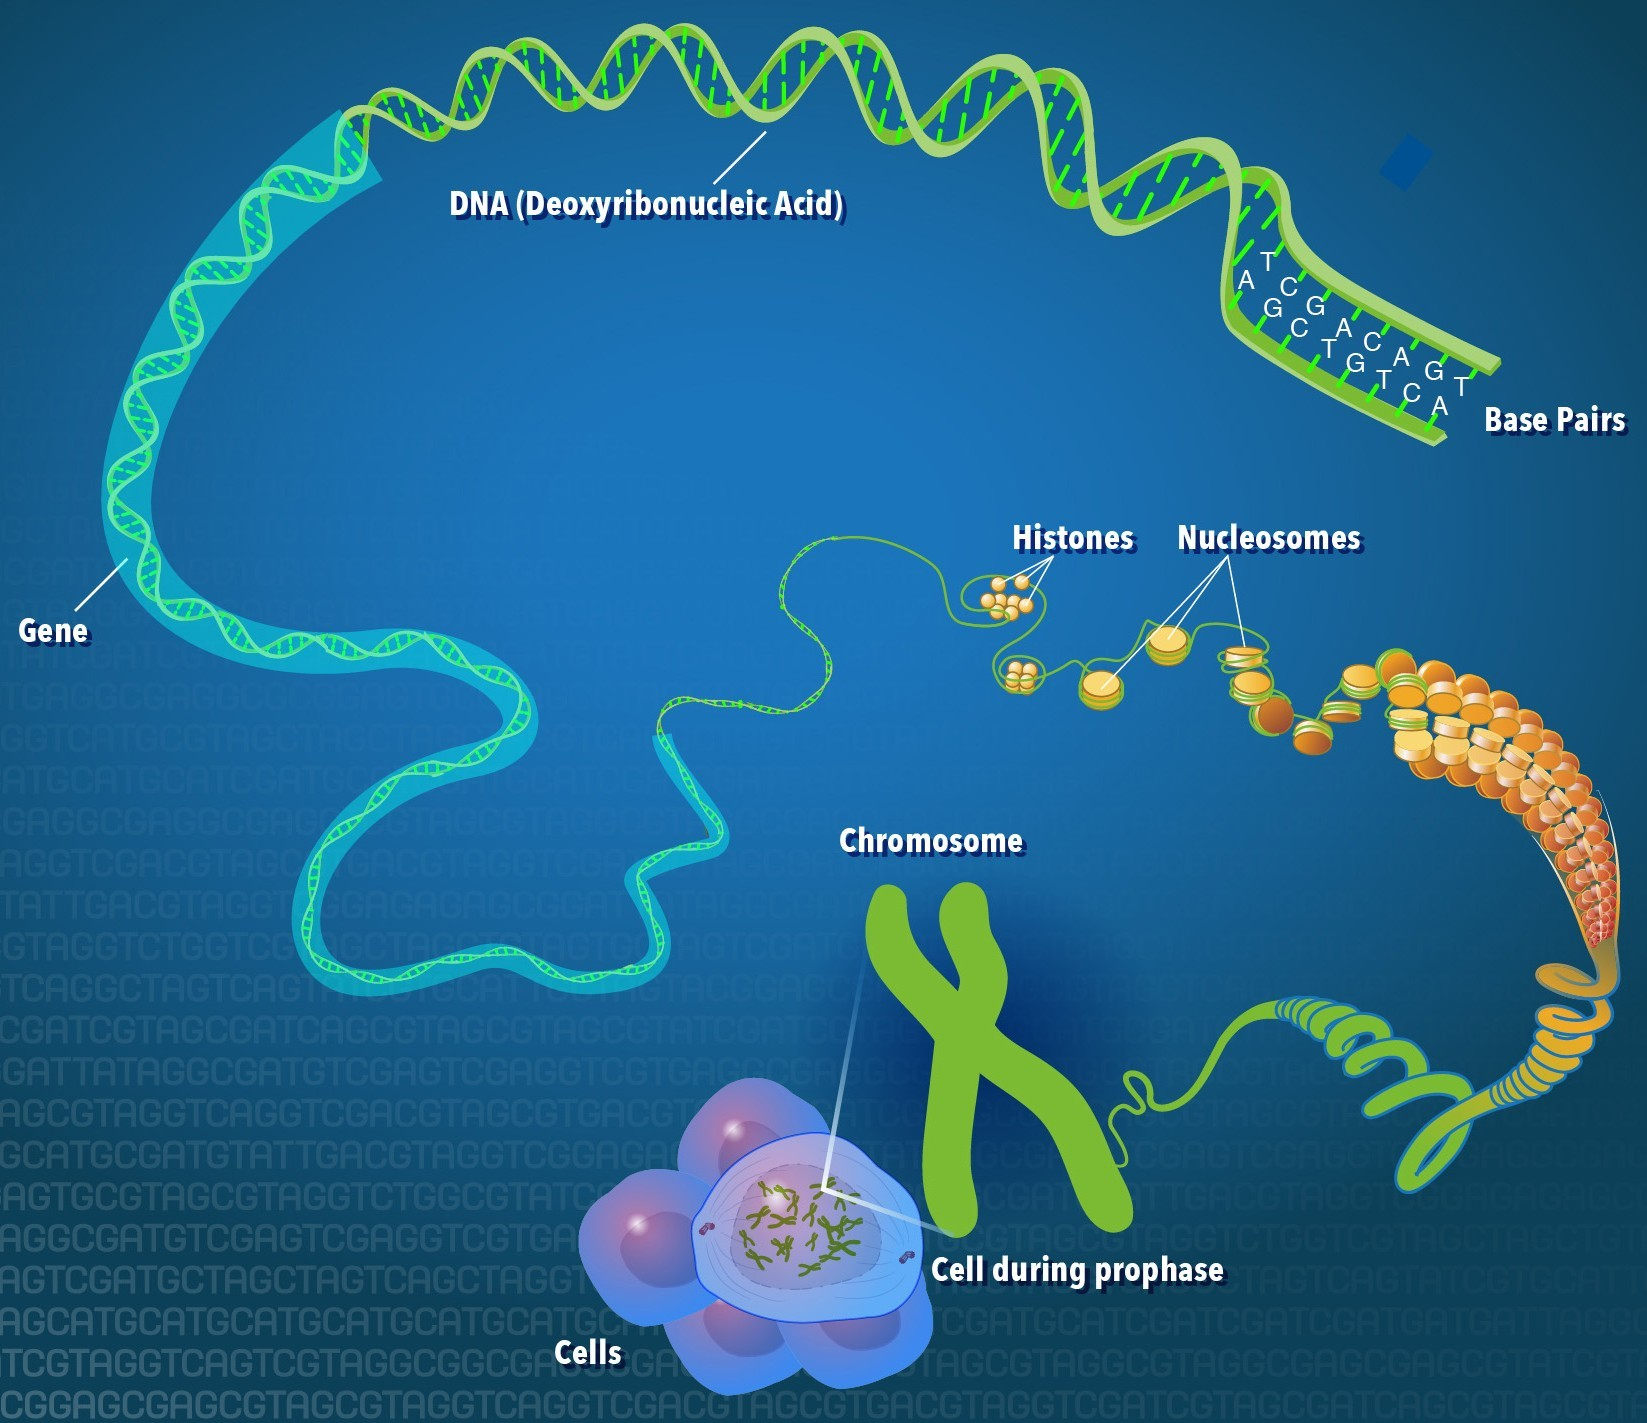
\includegraphics[width=0.7\textwidth]{c2.genomics.gene.01.jpg}
  \end{figure}
\end{frame}

\begin{frame}
  \frametitle{基因组学 | 概述 | 基因}
基因一词来自希腊语,意思为“生”。是指携带有遗传信息的DNA序列,是控制性状的基本遗传单位,亦即一段具有功能性的DNA序列。基因通过指导蛋白质的合成来表现所携带的遗传信息,从而控制生物个体的性状(差异)表现。人类约有两万至两万五千个基因。\\
\vspace{1em}
染色体在体细胞中是成对存在的,每条染色体上都带有一定数量的基因。一个基因在细胞有丝分裂时有两个对应的位点,称为等位基因,分别来自父与母。依所携带性状的表现,又可分为显性基因和隐性基因。\\
\vspace{1em}
一般来说,同一生物体中的每个细胞体都含有相同的基因,但并不是每个细胞中的所有基因携带的遗传信息都会被表现出来。职司不同功能的细胞中,活化而表现的基因也不同。
\end{frame}

\begin{frame}
  \frametitle{基因组学 | 概述 | 基因组}
在生物学中,一个生物体的基因组是指包含在该生物的DNA(部分病毒是RNA)中的全部遗传信息,又称基因体(genome)。基因组包括基因和非编码DNA。1920年,德国汉堡大学植物学教授汉斯·温克勒(Hans Winkler)首次使用基因组这一名词。\\
\vspace{1em}
更精确地讲,一个生物体的基因组是指一套染色体中的完整的DNA序列。例如,生物个体体细胞中的二倍体由两套染色体组成,其中一套DNA序列就是一个基因组。基因组一词可以特指整套核DNA(例如,核基因组),也可以用于包含自己DNA序列的细胞器基因组,如粒线体基因组或叶绿体基因组。当人们说一个有性生殖物种的基因组正在测序时,通常是指测定\textcolor{red}{一套常染色体和两种性染色体}的序列,这样来代表可能的两种性别。即使在只有一种性别的物种中,“一套基因组序列”可能也\textcolor{red}{综合了来自不同个体的染色体}。通常使用中,“遗传组成”一词有时在交流中即指某特定个体或物种的基因组。对相关物种全部基因组性质的研究通常被称为基因组学,该学科与遗传学不同,后者一般研究单个或一组基因的性质。
\end{frame}

\begin{frame}
  \frametitle{基因组学 | 概述 | 基因组}
对于像人类这样的脊椎动物,基因组通常指的只是染色体DNA。因此,尽管人类线粒体里包含了基因,但这些基因并不作为基因组的一部分。事实上,有时候称线粒体拥有自己的基因组,通常叫做\textcolor{red}{线粒体基因组}。而在叶绿体中的被称为\textcolor{red}{叶绿体基因组}。
\end{frame}

\begin{frame}
  \frametitle{基因组学 | 概述 | 基因组 | 测序}
  \begin{itemize}[<+->]
    \item 1976年,瓦尔特·菲尔斯(比利时根特大学)RNA病毒噬菌体MS2【第一个完整测序的基因组】
    \item 1977年,弗雷德里克·桑格,Φ-X174噬菌体【第一个完成测序的DNA基因组】
    \item 1995年,The Institute for Genomic Research团队,流感嗜血杆菌(\textit{Haemophilus influenzae})【第一个被测序的细菌基因组】
    \item 1996年,酿酒酵母(\textit{Saccharomyces cerevisiae})【第一个真核生物基因组】
    \item 1996年,The Institute for Genomic Research团队,詹氏甲烷球菌(\textit{Methanococcus jannaschii})【第一个被测序的古菌基因组】
    \item 1998年,秀丽隐杆线虫(\textit{Caenorhabditis elegans})【第一个被测序的多细胞生物基因组】
    \item 1990年,人类基因组计划启动
    \item 2007年,完成了詹姆斯·杜威·沃森个人基因组的测序
  \end{itemize}
\end{frame}

\begin{frame}
  \frametitle{基因组学 | 概述 | 基因组 | 补遗}
  \begin{block}{基因组构成}
基因组构成(genome composition)用于描述一个单倍体基因组的组成,包括基因组大小、非重复DNA和重复DNA所占的比重等。\\
\vspace{1em}
当讨论基因组的构成时,首先要区别的是原核基因组还是真核基因组,两者在基因组组成上有很大的不同。
  \end{block}
  \pause
  \begin{block}{基因组大小}
基因组大小是指一种生物单倍体基因组的全部DNA碱基对数。\\
\vspace{1em}
在原核生物和低等真核生物中,基因组大小与生物形态的复杂性基本呈正相关关系;但是在软体动物以及其它更高等的真核生物中,这种相关性就不存在了。这一现象可能是由基因组中的重复DNA引起的。 
  \end{block}
\end{frame}

\begin{frame}
  \frametitle{基因组学 | 概述 | 基因组 | 补遗}
  \begin{figure}
    \centering
    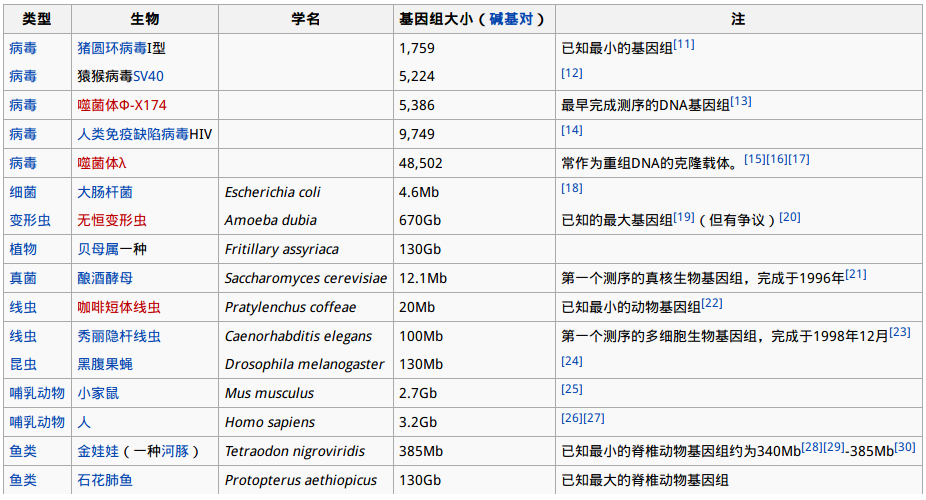
\includegraphics[width=\textwidth]{c2.genomics.genome.01.png}
  \end{figure}
\end{frame}

\begin{frame}
  \frametitle{基因组学 | 概述 | 基因组 | 补遗}
  \begin{block}{非重复DNA}
非重复DNA的总长除以基因组大小即为非重复DNA比重。蛋白质编码基因和非编码RNA基因一般都是非重复的DNA。\\
\vspace{1em}
不同生物中的非重复DNA的比重会有很大不同。更大的基因组并不意味着更多的基因,随着高等真核生物的基因组大小的增加,非重复DNA的比重相应减少。
  \end{block}
  \pause
  \begin{block}{基因组演化}
基因组不仅仅是是生物基因的集合,对其研究和比较能获得生物演化信息的更多细节。一些基因组性质如“染色体数”(核型)、基因组大小、基因顺序、密码子偏好性与GC含量能反映出现存生物的许多基因组演化信息。
  \end{block}
\end{frame}

\begin{frame}
  \frametitle{基因组学 | 概述 | 基因组学}
  \begin{block}{基因组学}
基因组学(genomics),或基因体学,是研究生物基因组和如何利用基因的一门学问。\\
\vspace{0.5em}
基因组学的主要工具和方法包括:生物信息学,遗传分析,基因表达测量和基因功能鉴定。
  \end{block}
  \pause
  \begin{block}{特点}
基因组学的特点是强调进行细胞中全部基因及非编码区的整体性考查和系统性研究,从而全面揭示基因与基因间的相互关系、基因与非编码序列的关系、基因与基因组的相互关系。
  \end{block}
\end{frame}

\begin{frame}
  \frametitle{基因组学 | 概述 | 基因组学}
  \begin{block}{组学}
“组”在基因组一词中,意指一个物种的“全部”遗传组成。由于诸如基因组测序这样的大规模定量生物项目的成功,“组”的这个意义的使用已经扩展到其他相关领域。例如,蛋白质组指的是一个物种组织或细胞内的全部蛋白质。 
  \end{block}
  \pause
  \begin{block}{基因组分析}
基因组项目涉及三个部分:DNA测序,该序列的组件生成原有染色体的表示法,以及该表示法的注释和分析。
  \end{block}
\end{frame}

\begin{frame}
  \frametitle{基因组学 | 概述 | 基因组学}
  \begin{itemize}[<+->]
    \item 1980年,噬菌体Φ-X174(5,368碱基对)完全测序,成为第一个测定的基因组
    \item 1995年,嗜血流感菌(Haemophilus influenzae,1.8Mb)测序完成,是第一个测定的自由生活物种
    \item 2001年,人类基因组计划公布了人类基因组草图,为基因组学研究揭开新的一页
    \item 2012年,千人基因组计划
  \end{itemize}
\end{frame}

\subsection{人类基因组计划}
\begin{frame}
  \frametitle{基因组学 | 概述 | 人类基因组}
  \begin{block}{人类基因组}
人类基因组,又称人类基因体,是智人的基因组,由\textcolor{red}{23对染色体}组成,其中包括\textcolor{red}{22对体染色体、1条X染色体和1条Y染色体}。人类基因组含有\textcolor{red}{约30亿个DNA碱基对},碱基对是以氢键相结合的两个含氮碱基,以胸腺嘧啶(T)、腺嘌呤(A)、胞嘧啶(C)和鸟嘌呤(G)四种碱基排列成碱基序列,其中A与T之间由两个氢键连接,G与C之间由三个氢键连接,碱基对的排列在DNA中也只能是A对T,G对C。其中一部分的碱基对组成了\textcolor{red}{大约20000到25000个基因}。 
  \end{block}
\end{frame}

\begin{frame}
  \frametitle{基因组学 | 概述 | 人类基因组}
  \begin{figure}
    \centering
    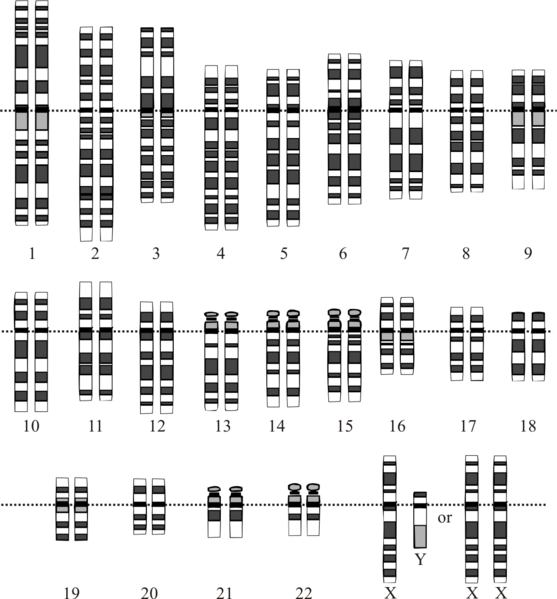
\includegraphics[width=0.6\textwidth]{c2.genomics.human.genome.01.png}
  \end{figure}
\end{frame}

\begin{frame}
  \frametitle{基因组学 | 概述 | 人类基因组 | 补遗}
  \begin{block}{染色体}
人类拥有23对不同的染色体,其中22对属于常染色体,另外还有1对能够决定性别的性染色体,分别是X染色体与Y染色体。1号到22号染色体的编号顺序,大致符合他们由大到小的尺寸排列。最大的染色体约含有2亿5千万个碱基对,最小的则约有3800万个碱基对。\\
\vspace{1em}
在人类个体的体细胞中,通常含有来自亲代的1到22对体染色体,再加上来自母亲的X染色体,以及来自父亲的X或Y染色体,总共是46个(23对)染色体。科学家将这些染色体分为7组:1号到3号是A组;4号与5号是B组;X染色体以及6号到12号是C组;13号到15号是D组;16号到18号是E组;19号与20号是F组;21号、22号与Y染色体是G组。对于一般人类来说,每个细胞核内只有两套染色体。
  \end{block}
\end{frame}

\begin{frame}
  \frametitle{基因组学 | 概述 | 人类基因组 | 补遗}
  \begin{block}{基因}
人体内估计约有20000到25000个蛋白质编码基因。虽然人类的基因数量比起某些较为原始的生物(如线虫与果蝇)更少,但是在人类细胞中使用了大量的选择性剪接(alternative splicing),这使得一个基因能够制造出多种不同的蛋白质,且人类的蛋白质组规模也较前述的两个物种更庞大。\\
\vspace{1em}
大多数人类基因拥有许多的外显子,且人类的内含子比位在其两端的外显子更长。这些基因参差不齐地分布在染色体中,每一个染色体皆含有一些基因较多的区段与基因较少的区段。这些区段的差异,则与染色体带(chromosome bands)及GC含量相关。基因密度所显现的非随机模式之涵义与重要性尚未明了。
  \end{block}
\end{frame}

\begin{frame}
  \frametitle{基因组学 | 概述 | 人类基因组 | 补遗}
  \begin{figure}
    \centering
    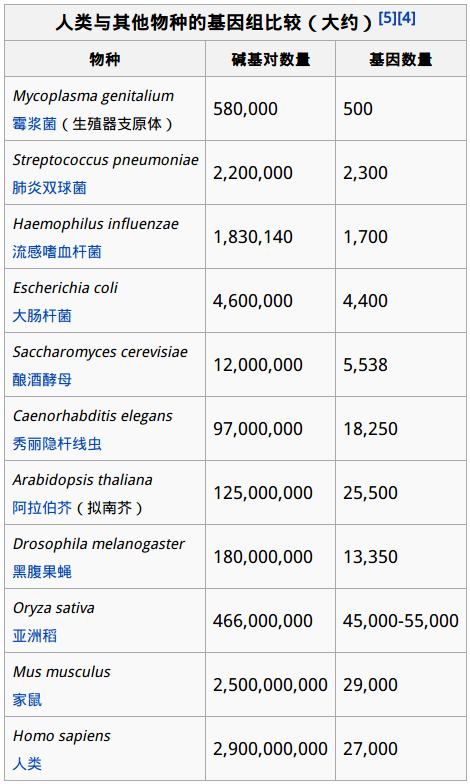
\includegraphics[width=0.38\textwidth]{c2.genomics.genome.size.01.png}
  \end{figure}
\end{frame}

\begin{frame}
  \frametitle{基因组学 | 概述 | 人类基因组 | 补遗}
  \begin{block}{功能未知区域}
    蛋白质编码序列(也就是外显子)在人类基因组中少于1.5\%。在基因与调控序列之外,仍然有许多功能未知的广大区域。科学家估计这些区域在人类基因组中约占有97\%,其中许多是属于重复序列(en:Repeated sequence (DNA))、转位子(transposon)与伪基因(pseudogene)。除此之外,还有大量序列不属于上述的已知分类。 \textcolor{red}{人类基因组内大量功能未知的序列,是目前科学研究的重点之一}。
  \end{block}
\end{frame}

\begin{frame}
  \frametitle{基因组学 | 概述 | 人类基因组 | 补遗}
  \begin{block}{变异}
    大多数对于人类遗传变异的研究集中在\textcolor{red}{单核苷酸多态性(single nucleotide polymorphisms;SNPs)},也就是DNA中的个别碱基变换。在人类的真染色质(富含基因的染色质)中,平均每100到1000个碱基会出现1个SNPs,不过密度并不均匀。由于SNPs的存在,如“所有人类的基因有99\%都是相同的”这样的说法并不精确。国际人类基因组单体型图计划(International HapMap Project),便是为了要将人类基因组中的SNP变异作编录,而组成的一个大规模合作计划。\\
\vspace{1em}
研究人员发现在人类与其他哺乳类DNA序列中的\textcolor{red}{拷贝数变异(copy number variation;CNV)},可能非常重要。拷贝数变异又称为拷贝数多型性(copy number polymorphisms;CNPs),是缺失(deletion)、插入(insertion)、重复(duplication),以及复杂多位置变异(complex multi-site variants)的合称,在所有人类以及其他已测试的哺乳动物中皆可发现。
  \end{block}
\end{frame}

\begin{frame}
  \frametitle{基因组学 | 概述 | 人类基因组 | 补遗}
  \begin{block}{演化}
比较基因组学(Comparative genomics)对于哺乳类基因组的研究显示,人类与大约两亿年前就已经分化的各物种相比,有大约5\%的比例在人类基因组中保留了下来,其中包含许多的基因与调控序列。而且人类与大多数已知的脊椎动物间,也享有了一些相同的基因。\\
 \vspace{1em}
黑猩猩的基因组与人类的基因组之间,有98.77\%是相似的。而平均每一个属于人类的标准蛋白质编码基因,只与属于黑猩猩的同源基因相差两个氨基酸;并且有将近三分之一的人类基因与黑猩猩的同源基因,能够翻译出相同的蛋白质。人类的2号染色体,是人类与黑猩猩基因组之间的主要差异,它是由黑猩猩的染色体12号与13号融合而成的。\\
 \vspace{1em}
人类在最近的演化过程中失去了嗅觉受体基因,这解释了为何人类比起其他的哺乳动物来说,拥有较差的嗅觉。演化上的证据显示,人类与某些灵长类所拥有的彩色视觉,降低了这些物种对于嗅觉能力的需求。
  \end{block}
\end{frame}

\begin{frame}
  \frametitle{基因组学 | 概述 | 人类基因组 | 补遗}
  \begin{block}{线粒体基因组}
大多数的基因是存在细胞核中,但是细胞中一个称为线粒体的细胞器,也拥有自己的基因组。线粒体基因组在线粒体疾病(mitochondrial disease)中具有一定的重要性;而且这些基因也可以用来研究人类的演化。线粒体位于细胞质中,当人类的精子与卵子结合时,源自母亲(女性)的卵子提供了绝大多数的细胞质,因此人类细胞中的线粒体基因皆是来自母亲。\\
\vspace{1em}
由于线粒体缺乏用来检查复制错误的能力,因此\textcolor{red}{线粒体DNA(mDNA)}的变异速率比细胞核DNA(一般所指的DNA)更快。线粒体的突变速率快了20倍,这使mDNA能够用来较为精确地追溯出母系祖先。研究族群中的mDNA,也能使人们得知此族群过去的迁移路径。
  \end{block}
\end{frame}

\begin{frame}
  \frametitle{基因组学 | 概述 | 人类基因组计划}
  \begin{figure}
    \centering
    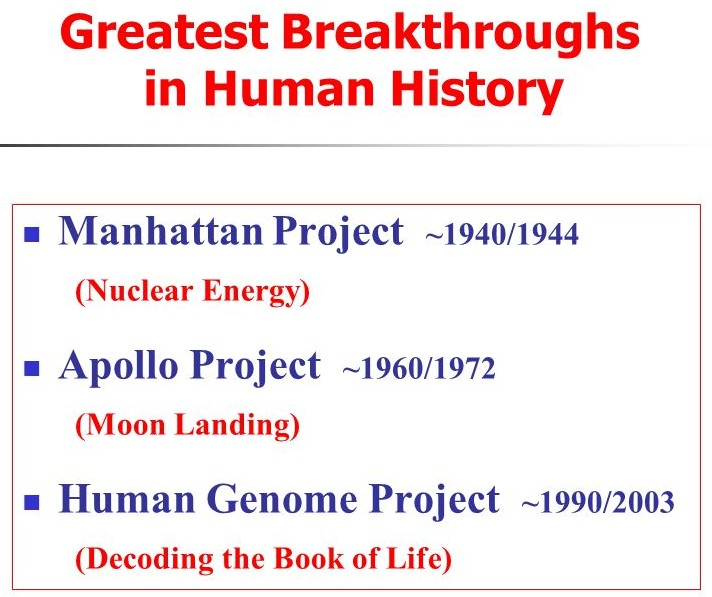
\includegraphics[width=0.7\textwidth]{c2.genomics.hgp.01.jpg}
  \end{figure}
\end{frame}

\begin{frame}
  \frametitle{基因组学 | 概述 | 人类基因组计划}
人类基因组计划(human genome project, HGP)是一项规模宏大,跨国跨学科的科学探索工程。其宗旨在于测定组成人类染色体(指单倍体)的30亿个碱基对形成的核苷酸序列,从而绘制人类基因组图谱,并且辨识其载有的基因,达到破译人类遗传信息的最终目的。\\
\vspace{1em}
该计划起始于1990年,已基本测序了人类的所有基因。截止到2005年,人类基因组计划的测序工作已经基本完成(92\%)。但关于其功能的细节,则仍有许多研究在进行中。\\
\vspace{1em}
其中,2001年人类基因组工作草图的发表被认为是人类基因组计划成功\textcolor{red}{【?】}的里程碑。
\end{frame}

\begin{frame}
  \frametitle{基因组学 | 概述 | 人类基因组计划 | 事件}
  \begin{itemize}[<+->]
    \item 1984年,第一次讨论人类基因组测序的价值
    \item 1985年,首次对于人类基因组测序的可行性进行认真的探讨
    \item 1986年,罗纳德·杜尔贝科(Renato Dulbecco),建议开展人类基因组研究计划
    \item 1986年,美国能源部(DOE)加入人类基因组计划
    \item 1987年,美国国家卫生研究院(NIH)加入人类基因组计划
    \item 1998年,詹姆士·华生,NIH的基因组部门主管(1988-1992)
    \item 1988年,国际人类基因组组织(HUGO)成立
  \end{itemize}
\end{frame}

\begin{frame}
  \frametitle{基因组学 | 概述 | 人类基因组计划 | 事件(续)}
  \begin{itemize}[<+->]
    \item 1990年,投资30亿美元的人类基因组计划由美国能源部和国家卫生研究院正式启动,预期在15年内完成,随后扩展为国际合作的人类基因组计划
    \item 1996年,百慕大会议,以2005年完成测序为目标,分配了各国负责的工作,并且宣布研究结果将会即时公布,且完全免费
    \item 1998年,克莱格·凡特的塞雷拉基因组公司成立,希望能以更快的速度和更少的投资(3亿美元)来完成此项工程;开发出全世界第一台全自动测序仪,宣布将在2001年完成测序工作
    \item 2000年6月26日,塞雷拉公司的代表凡特,以及国际合作团队的代表弗朗西斯·柯林斯(Francis Collins),在美国总统克林顿的陪同下发表演说,宣布人类基因组的概要已经完成;所有人类基因组数据为人类共同财产,不允许专利保护,且必须对所有研究者公开
    \item 2001年2月,国际人类基因组测序联盟与塞雷拉公司,分别将研究成果发表于《自然》与《科学》;覆盖基因组序列的83%,包括常染色质区域的90%(带有150,000个空缺,且许多片断的顺序和方位并没有得到确定)
  \end{itemize}
\end{frame}

\begin{frame}
  \frametitle{基因组学 | 概述 | 人类基因组计划 | 事件 | 中国}
  \begin{itemize}[<+->]
    \item 1994年,中国的人类基因组计划启动
    \item 1998年,中国南方基因组中心成立,中国科学院遗传研究所人类基因组中心成立
    \item 1999年,北京华大基因研究中心(华大基因)成立,北方基因组中心成立
    \item 1998年3月,中美港科学家合作,成功地将与华人和鼻咽癌有关的肿瘤抑制基因定位于人类第3号染色体的短臂3p21.3位点
    \item 1999年6月26日,中国科学院遗传研究所人类基因组中心向美国国立卫生研究院(NIH)的国际人类基因组计划(HGP)递交加入申请。HGP在网上公布中国注册加入国际测序组织,中国成为继美、英、日、德、法后第六个加入该组织的国家
    \item 1999年11月10日,1\%计划被列入中国国家项目,并确定由北京华大基因研究中心(华大基因)牵头,国家基因组南方中心、北方中心共同参与,承担全部工程1%的测序工作
    \item 2000年4月,中国完成了人第3号染色体上3000万个碱基对的工作草图
  \end{itemize}
\end{frame}

\begin{frame}
  \frametitle{基因组学 | 概述 | 人类基因组计划 | 事件}
  \begin{figure}
    \centering
    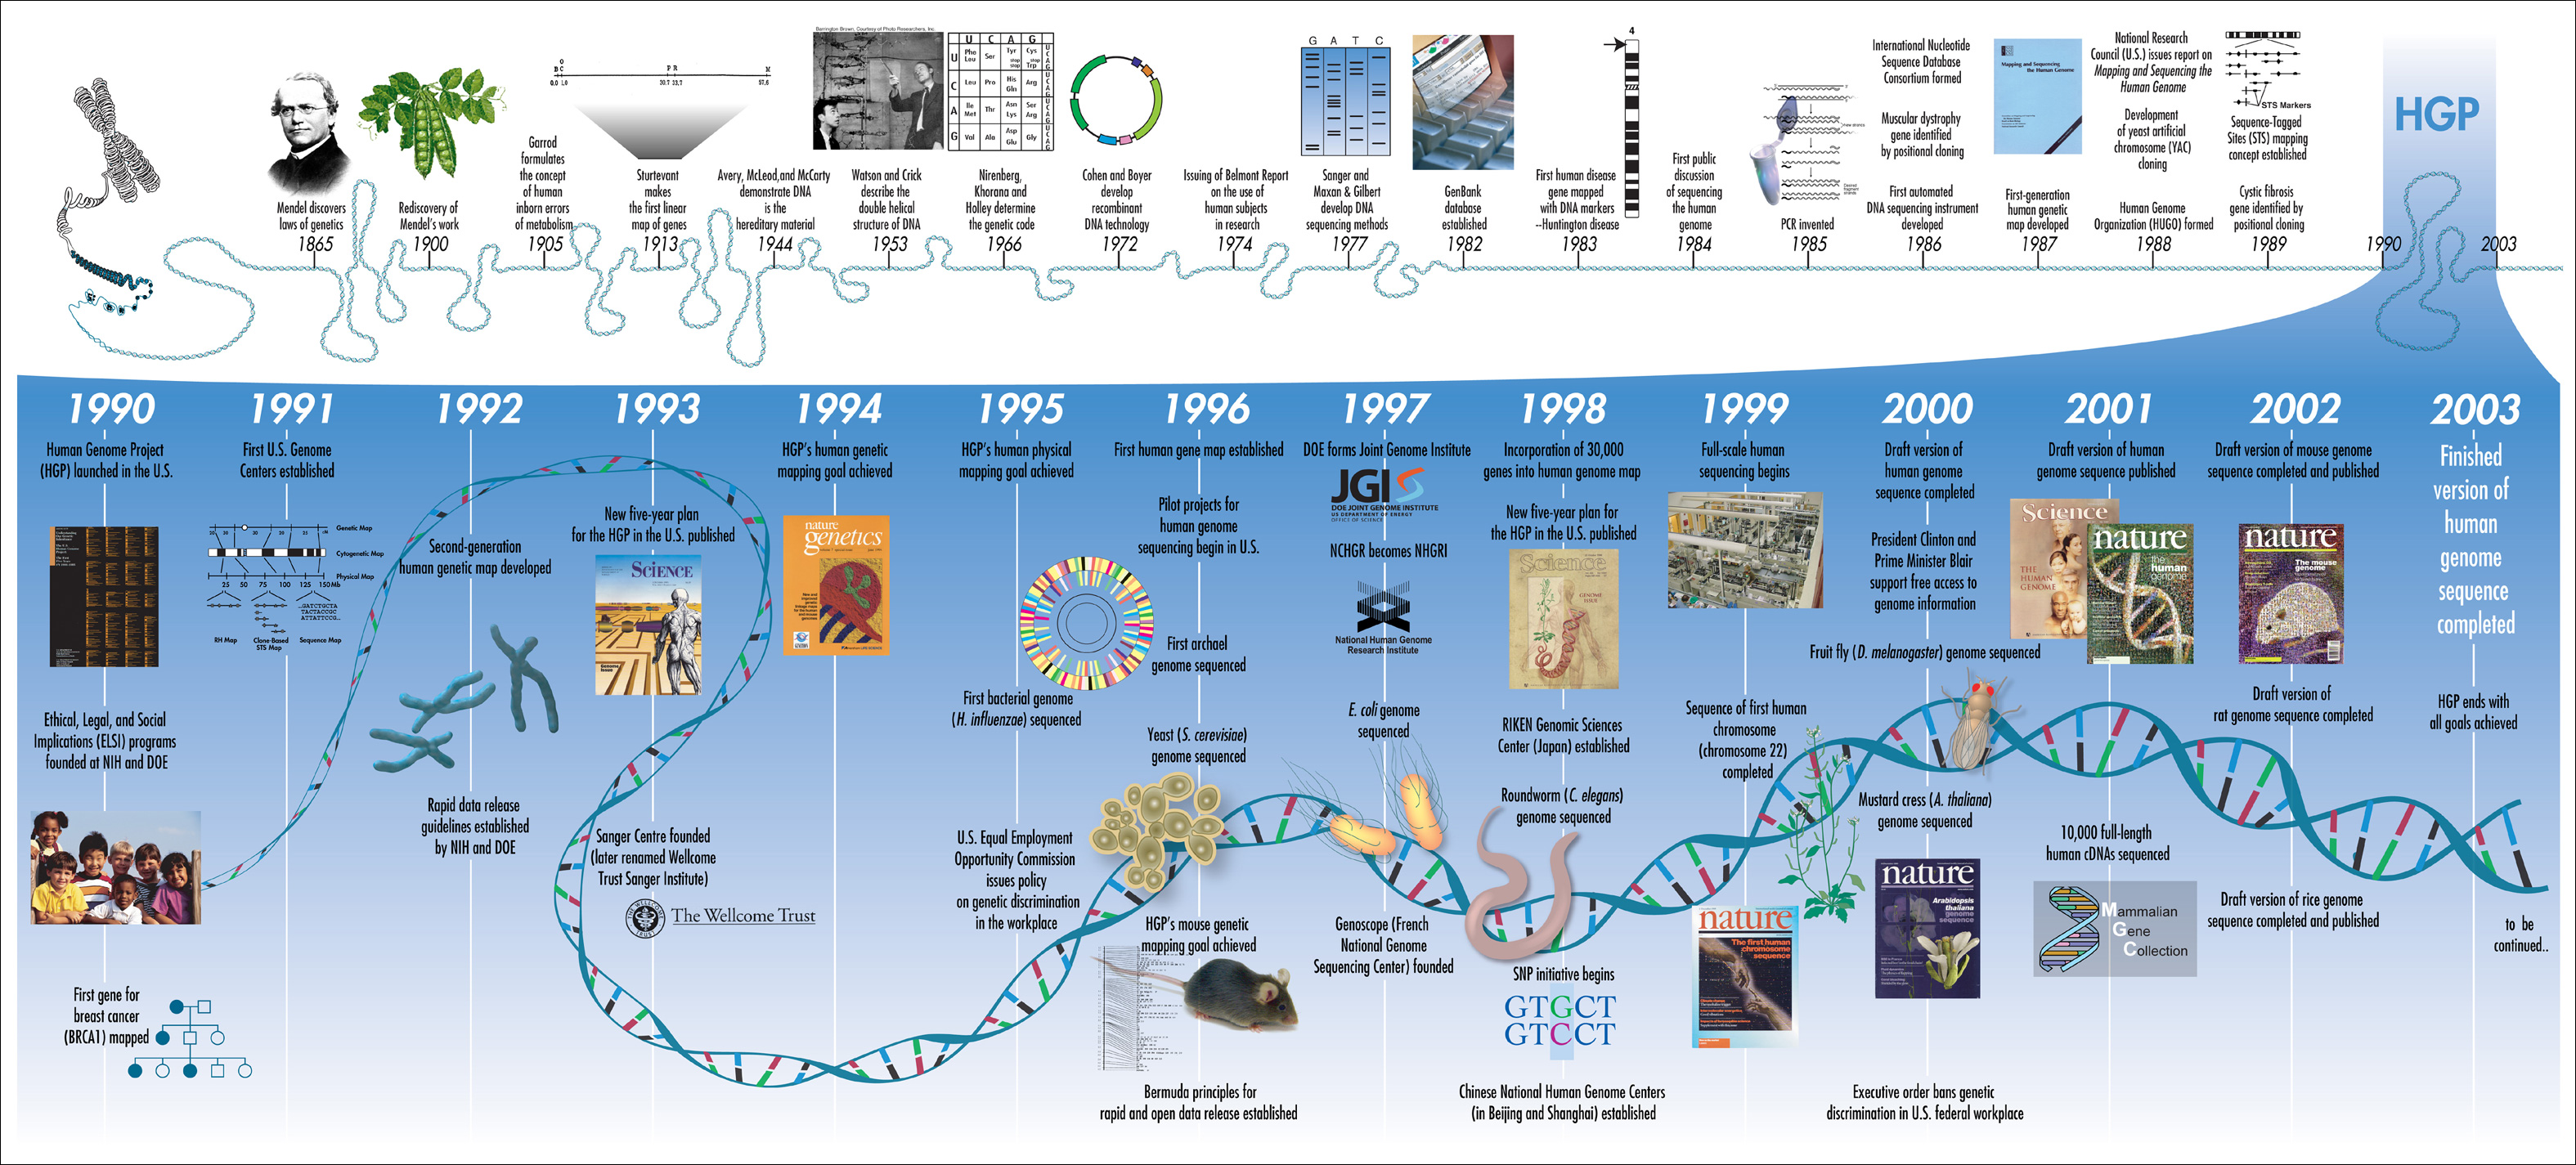
\includegraphics[width=\textwidth]{c2.genomics.hgp.timeline.01.jpg}
  \end{figure}
\end{frame}

\begin{frame}
  \frametitle{基因组学 | 概述 | 人类基因组计划 | 目标}
  \begin{description}[<+->]
    \item[遗传图谱的绘制] 遗传图谱主要是用遗传标签来确定基因在染色体上的排列。 
    \item[物理图谱的绘制] 物理图谱是通过序列标签位点对构成基因组的DNA分子进行测定,从而对某基因所相对之遗传讯息及其在染色体上的相对位置做一线性排列。
    \item[序列测定] 通过测序得到基因组的序列,是一般意义上的人类基因组计划。 
    \item[辨别序列中的个体差异] 人类基因组计划只是为未来鉴定不同个体间基因组差异做一些基础的框架性工作。当前主要工作在于鉴定不同个体间包含的单核苷酸多态性。
    \item[基因鉴定] 以获得全长的人类cDNA文库为目标。
    \item[基因的功能性分析] 对海量的数据进行标注,分析注释序列。另一个目标是研发出更快更有效的方法来进行DNA测序和序列分析,并把这一技术加以产业化。 
  \end{description}
\end{frame}

\begin{frame}
  \frametitle{基因组学 | 概述 | 人类基因组计划 | 目标 | 完成情况}
  \begin{description}[<+->]
    \item[遗传图谱的绘制] 1994年9月,完成了包含3000个(原计划为600-1500)标签分辨率为1-cM(即1\%重组率)的遗传图谱的绘制。
    \item[物理图谱的绘制] 1998年10月,完成了包含52,000个(原计划为30,000)序列标签位点的物理图谱的绘制。
    \item[序列测定] 2003年4月,包含基因序列中的98%(原预计为95%)获得了测定,精确度为99.99%。
    \item[辨别序列中的个体差异] 至2003年2月,已有约3,700,000个单核苷酸多态性位点得到测定。
    \item[基因鉴定] 至2003年3月,已获得15,000个全长的人类cDNA文库。
    \item[基因的功能性分析] 已获得开发的技术包括高通量寡聚核苷酸的合成(1994年)、DNA微阵列(1996年)、标准化和消减化cDNA文库(1996年)、真核(酵母)全基因组敲除技术(1999年)、大型化双杂交定位(2002年)。
  \end{description}
\end{frame}

\begin{frame}
  \frametitle{基因组学 | 概述 | 人类基因组计划 | 图谱}
  \begin{block}{遗传图谱}
遗传图谱(genetic map)是利用基因的重组率来做分析,单位是分莫甘(centimorgan)。这种图谱表现出来的是基因或特定DNA片段之间的相对位置,而不是它们各自的绝对位置。
  \end{block}
  \pause
  \begin{block}{物理图谱}
物理图谱(physical map)则是DNA两点的实际距离,是实际将DNA片段排序而得,单位是碱基的数目(如Kb;kilobase)。
  \end{block}
\end{frame}

\begin{frame}
  \frametitle{基因组学 | 概述 | 人类基因组计划 | 完成?}
  \begin{block}{完成}
关于如何界定人类基因组测序完成,有多种定义。根据不同的定义,人类基因组的测序是否完成有不同的看法。曾有多个大众媒体报道人类基因组计划“完成”,而且由国际人类基因组计划所采用的定义,基因组的测序已经完成。
  \end{block}
  \pause
  \begin{block}{仍有许多的区域未获得测序}
    \begin{itemize}
      \item 着丝粒含有数百万(可能接近千万)的碱基对,其中的大多数完全没有得到测序
      \item 染色体末端区域(称为端粒)大都不完整,无法精确地知道在端粒前还有多少序列
      \item 每个人的基因组中都含有多个包含多基因家族成员的位点
      \item 还有一些间隙散布于基因组中,部分间隙较大
    \end{itemize}
  \end{block}
\end{frame}

\begin{frame}
  \frametitle{基因组学 | 概述 | 人类基因组计划 | 意义}
  \begin{itemize}
    \item 基础科研领域:癌症、老年痴呆症等疾病的病因研究,推动新的疗法和新药的开发研究
    \item 医疗健康/商业价值:基因检测,个性化医疗/精准医疗
    \item 生物进化研究:揭示了许多重要的生物进化史上的里程碑事件(核糖体的出现,器官的产生,胚胎的发育,脊柱和免疫系统等)
    \item 人类遗传信息的应用:考古学(走出非洲),犯罪学以及社会执法
  \end{itemize}
\end{frame}

\begin{frame}
  \frametitle{基因组学 | 概述 | 人类基因组计划 | 补遗}
  \begin{itemize}
    \item 2004年,国际人类基因组测序联盟的研究者宣布,人类基因组中所含基因的预计数目从先前的30,000至40,000(在计划初期的预计数目则高达2,000,000)调整为20,000至25,000。预期还需要多年的时间来确定人类基因组中所含基因的精确数目。
    \item 目前基因组信息的注释工作仍然处于初级阶段。
  \end{itemize}
\end{frame}

\begin{frame}
  \frametitle{基因组学 | 概述 | 人类基因组计划 | 补遗}
  \begin{block}{延伸计划}
    \begin{description}
      \item[模式生物的基因组计划] 小鼠、果蝇、线虫、斑马鱼、酵母等
      \item[人类元基因组计划] 对人体内所用共生菌群的基因组进行序列测定,并研究与人体发育和健康相关基因的功能
      \item[国际人类基因组单体型图计划(HapMap计划)] 目标是构建人类DNA序列中多态位点的常见模式,为研究人员确定对健康和疾病以及对药物和环境反应有影响的相关基因提供关键信息 
      \item[人类基因组多样性研究计划] 对不同人种、民族、人群的基因组进行研究和比较,这一计划将为疾病监测、人类的进化研究和人类学研究提供重要信息
      \item[千人基因组计划(1000 Genomes Project)] 目标是建立最详尽的人类遗传变异目录。启动于2008年1月,计划在随后三年内,测定来自不同族群的数量至少一千名的匿名参与者的基因组序列。2010年完成试点阶段,2012年10月公布1092个基因组的测序
    \end{description}
  \end{block}
\end{frame}

\subsection{分支学科}
\begin{frame}
  \frametitle{基因组学 | 概述 | 分支学科 | 结构基因组学}
  \begin{block}{结构基因组学}
结构基因组学(Structural Genomics)是基因组学的一个重要组成部分和研究领域,它是一门通过基因作图、核苷酸序列分析确定基因组成、基因定位的科学。
  \end{block}
\end{frame}

\begin{frame}
  \frametitle{基因组学 | 概述 | 分支学科 | 功能基因组学}
  \begin{block}{功能基因组学}
功能基因组学(Functional genomics)的研究又往往被称为后基因组学(Postgenomics)研究,它是利用结构基因组学提供的信息和产物,在基因组或系统水平上全面分析基因的功能和相互作用。\\
\vspace{1em}
功能基因组学是利用结构基因组学所获得的各种信息,建立与发展各种技术和实验模型来测定基因及基因非编码序列的生物学功能。
  \end{block}
\end{frame}

\begin{frame}
  \frametitle{基因组学 | 概述 | 分支学科 | 功能基因组学}
  \begin{figure}
    \centering
    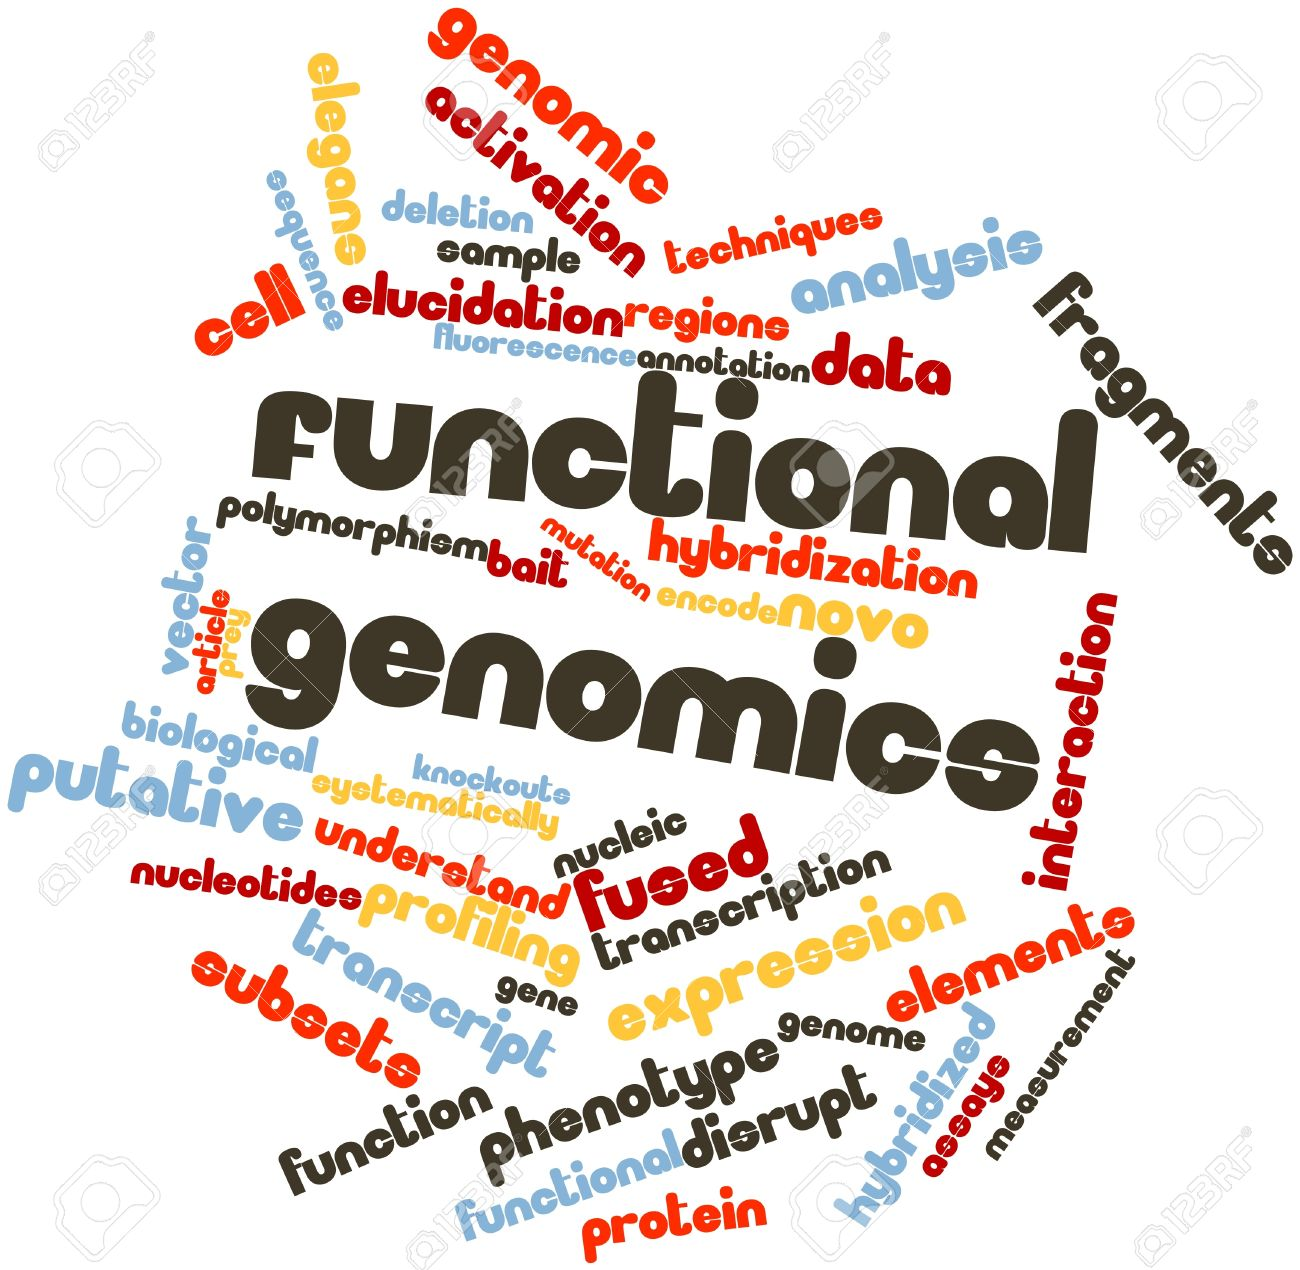
\includegraphics[width=0.65\textwidth]{c2.genomics.functional.genomics.02.jpg}
  \end{figure}
\end{frame}

\begin{frame}
  \frametitle{基因组学 | 概述 | 分支学科 | 比较基因组学}
  \begin{block}{比较基因组学}
比较基因组学(Comparative genomics)是在基因组图谱和测序技术的基础上,对已知的基因特征和基因组结构进行比较以了解基因的功能、表达机制和不同物种亲缘关系的生物学研究。比较基因组学的基础是相关生物基因组的相似性。全基因组比对是比较基因组学的经典方法。比较基因组学的研究成果催生了水平基因转移理论,支持细胞器起源的内共生学说。\\
\vspace{1em}
比较基因组学是研究比较不同物种基因组的异同,目的在于寻找物种间共有的、也就是在进化上保守的基因或DNA序列,这些基因往往具有重要的生物学功能。也可以从这些模式生物中寻找人类可能具有的新基因,以及为预测新的基因功能提供依据。
  \end{block}
\end{frame}

\begin{frame}
  \frametitle{基因组学 | 概述 | 分支学科 | 比较基因组学}
  \begin{figure}
    \centering
    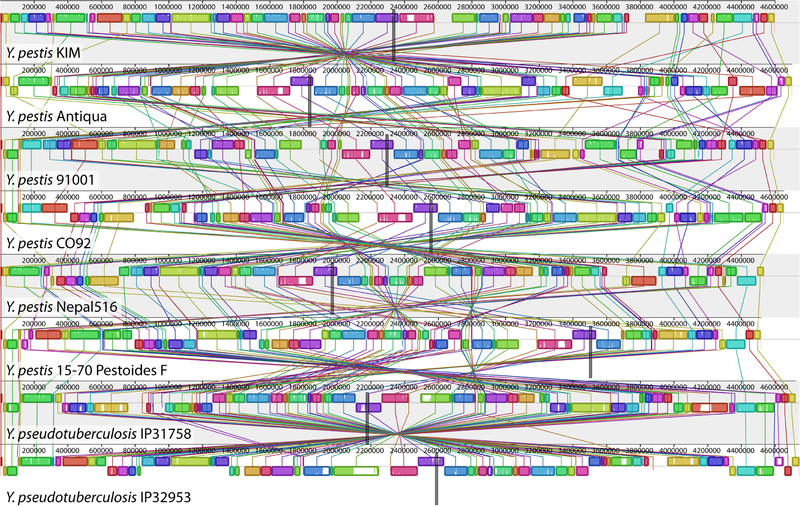
\includegraphics[width=0.9\textwidth]{c2.genomics.comparative.genomics.01.png}
  \end{figure}
\end{frame}

\begin{frame}
  \frametitle{基因组学 | 概述 | 分支学科 | 比较基因组学 | 种间}
  \begin{block}{种间比较基因组学研究}
通过对不同亲缘关系物种的基因组序列进行比较,能够鉴定出编码序列、非编码调控序列及给定物种独有的序列。而基因组范围之内的序列比对,可以了解不同物种在核苷酸组成、同线性关系和基因顺序方面的异同,进而得到基因分析预测与定位、生物系统发生进化关系等方面的信息。
  \end{block}
\end{frame}

\begin{frame}
  \frametitle{基因组学 | 概述 | 分支学科 | 比较基因组学 | 种内}
  \begin{block}{种内比较基因组学研究}
同种群体内基因组存在大量的变异和多态性,正是这种基因组序列的差异构成了不同个体与群体对疾病的易感性和对药物与环境因子不同反应的遗传学基础。
\begin{itemize}
  \item 单核苷酸多态性(single-nucleotide polymorphism,SNP)是指在基因组水平上由于单个核苷酸位置上存在转换或颠换等变异所引起的DNA序列多态性。
  \item 拷贝数多态性(copy number polymorphism,CNP):平均2个个体间存在11个CNP的差异,CNP的平均长度为465kb,其中半数以上的CNP在多个个体中重复出现,并经常定位于其他类型的染色体重排附近。
\end{itemize}
  \end{block}
\end{frame}

\begin{frame}
  \frametitle{基因组学 | 概述 | 分支学科 | 比较基因组学 | 研究方法}
  \begin{block}{系统发育谱法}
系统发育谱法(phylogenetic profile method)是在基因组全序列已完成测序的一系列基因组中分析某一蛋白质存在与否的模式。如果两个蛋白质在所研究的若干基因组中有相同的系统发育谱,便推断这两个蛋白质具有功能联系。
  \end{block}
  \pause
  \begin{block}{基因邻居法}
    基因邻居法(gene neighbour method)的原理是原核生物中如果两个基因在一个共同的操纵子内,且在不同的其他基因组也出现相邻现象,就可以推断它们编码的蛋白质之间具有功能联系。
  \end{block}
\end{frame}

\begin{frame}
  \frametitle{基因组学 | 概述 | 分支学科 | 比较基因组学 | 研究方法}
  \begin{figure}
    \centering
    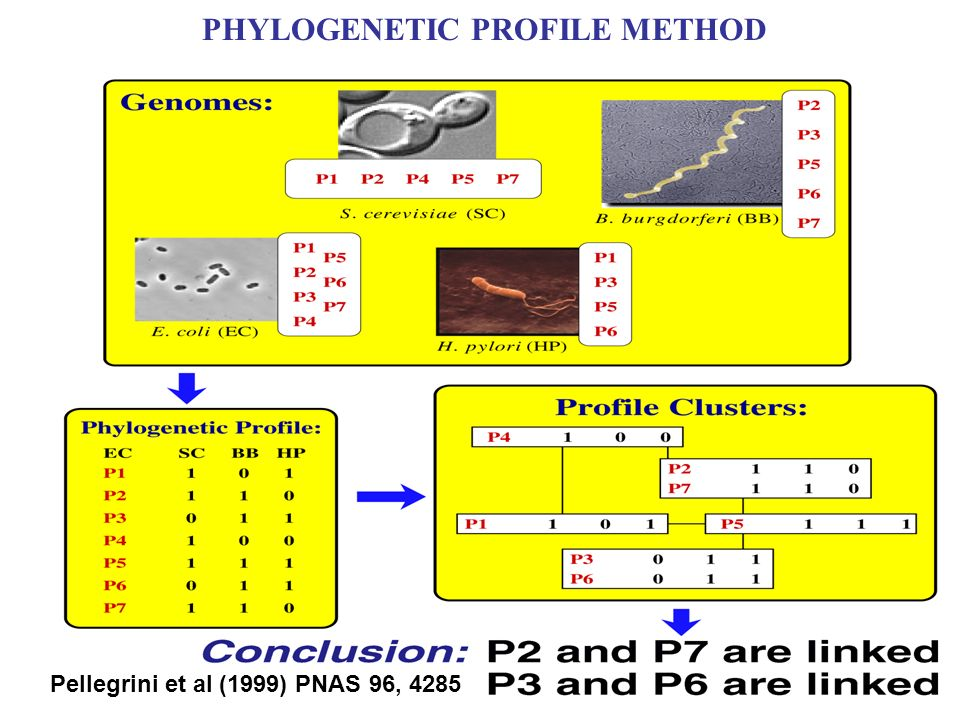
\includegraphics[width=0.9\textwidth]{c2.genomics.comparative.genomics.ppm.01.jpg}
  \end{figure}
\end{frame}

\begin{frame}
  \frametitle{基因组学 | 概述 | 分支学科 | 比较基因组学 | 研究方法}
  \begin{figure}
    \centering
    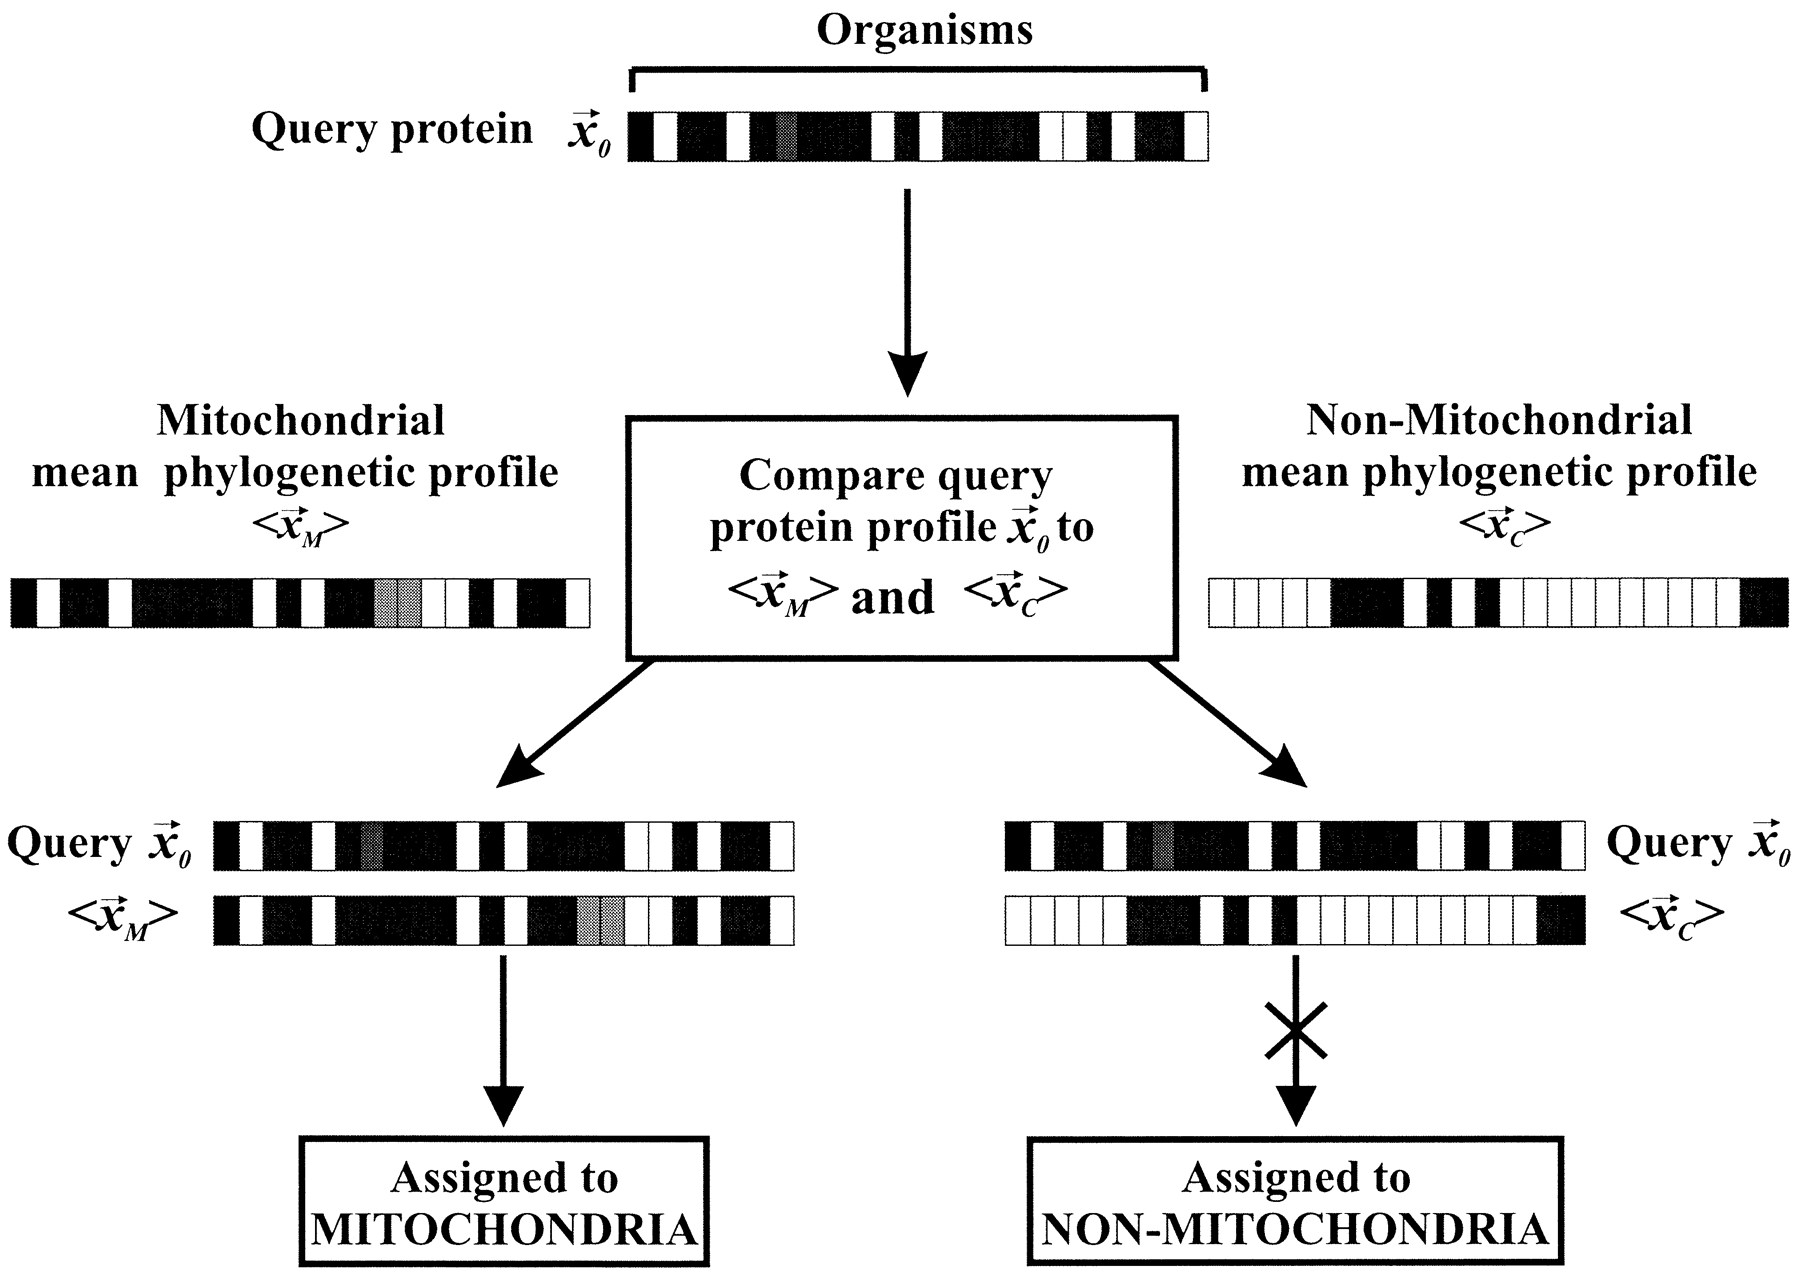
\includegraphics[width=0.9\textwidth]{c2.genomics.comparative.genomics.ppm.02.jpg}
  \end{figure}
\end{frame}

\begin{frame}
  \frametitle{基因组学 | 概述 | 分支学科 | 药物基因组学}
  \begin{block}{药物基因组学}
药物基因组学旨在理解个体对药物不同反应的遗传北京,即为什么某种药物对一部分人群有效,而对另一部分人群效果不佳或完全失效。\\
\vspace{1em}
制药业将充分应用药物基因组学的理论知识和技术手段来设计临床实验并模拟和分析理论与实验数据,也为新药设计和筛选提供依据。
  \end{block}
\end{frame}

\begin{frame}
  \frametitle{基因组学 | 概述 | 分支学科 | 药物基因组学}
  \begin{block}{个体对药物不同反应的遗传背景研究}
人类基因组DNA在个体间一般呈现0.01\%差异,几乎每个基因都有一个核苷酸变异谱。这是人类个体对药物敏感性不同的遗传基础,也是现代医学提出药物治疗必须个体化的依据。
  \end{block}
  \pause
  \begin{block}{为药物设计和筛选提供依据}
现代药物设计应考虑与遗传有关的若干因素:
\begin{itemize}
  \item 与致病有关的等位基因常会影响到对药物作用的反应
  \item 药物代谢途径与疗效密切相关
\end{itemize}
  \end{block}
\end{frame}

\begin{frame}
  \frametitle{基因组学 | 概述 | 分支学科 | 元基因组学}
  \begin{block}{元基因组学}
元基因组或总体基因组学(Metagenomics)是一门直接取得环境中所有遗传物质的研究,意指直接研究环境中微生物群落基因体学的应用,而非于实验室中进行单一个体纯化与培养的实验方式。研究领域广泛,也可称为环境基因组学、生态基因组学或群落基因组学。\\
\vspace{1em}
在早期研究微生物基因体必须将环境基因DNA或RNA克隆进入大肠杆菌体内,利用复制扩增方式,分析在自然环境中复制扩增特定基因(通常为16S rRNA)的多样性。但是,以复制扩增的方式得不到精准的微生物多样性。总体基因体学是认识复杂微生物群落的主要途径,提供一个更客观的方式发现微生物的世界,有可能改变之前我们所认知的微生物世界。
  \end{block}
\end{frame}

\begin{frame}
  \frametitle{基因组学 | 概述 | 分支学科 | 元基因组学}
  \begin{figure}
    \centering
    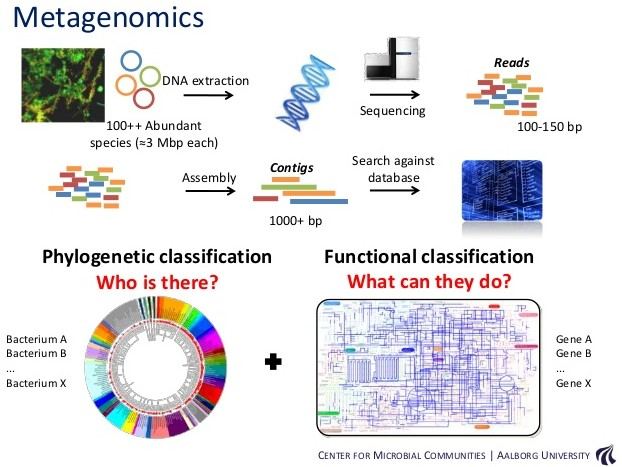
\includegraphics[width=0.8\textwidth]{c2.genomics.metagenomics.01.jpg}
  \end{figure}
\end{frame}

\begin{frame}
  \frametitle{基因组学 | 概述 | 分支学科 | 元基因组学 | 人体元基因组}
人类元基因组是指与人类共生的全部微生物的基因总和。又被称为“微生物组”或“人类第二基因组”。\\
\vspace{1em}
人类体内的微生物多达1000多种,特别是胃肠道内的微生物最为丰富;因此我们所说的元基因组在狭义上指的是肠道源基因组。\\
\vspace{1em}
人体内微生物的编码基因的总量大约是人类编码基因数目的50-100倍,这相当于在人类体内存在着另一个基因组通过表达调控人体的生命健康,即第二基因组。\\
\vspace{1em}
目前关于元基因组的研究还处于一个比较浅的阶段,在现有的研究中普遍认为糖尿病和肥胖症与人体元基因组有关。\\
\vspace{1em}
美国国立卫生研究院在2007年启动人体微生物计划,这计划一开始最主要的目的是调查是否有人体微生物的存在、了解人体微生物的变化与人类健康的关系,并开发新的技术和生物资讯的工具以支持这些目标。
\end{frame}


\section{测序技术}
\begin{frame}
  \frametitle{基因组学 | 测序 | 简介}
  \begin{block}{DNA测序}
DNA测序(DNA sequencing)是指分析特定DNA片段的碱基序列,也就是腺嘌呤(A)、胸腺嘧啶(T)、胞嘧啶(C)与鸟嘌呤(G)的排列方式。
  \end{block}
  \pause
  \begin{block}{RNA测序}
RNA测序则通常将RNA提取后,反转录为DNA后使用DNA测序的方法进行测序。
  \end{block}
\end{frame}

\begin{frame}
  \frametitle{基因组学 | 测序 | 历史}
  \begin{figure}
    \centering
    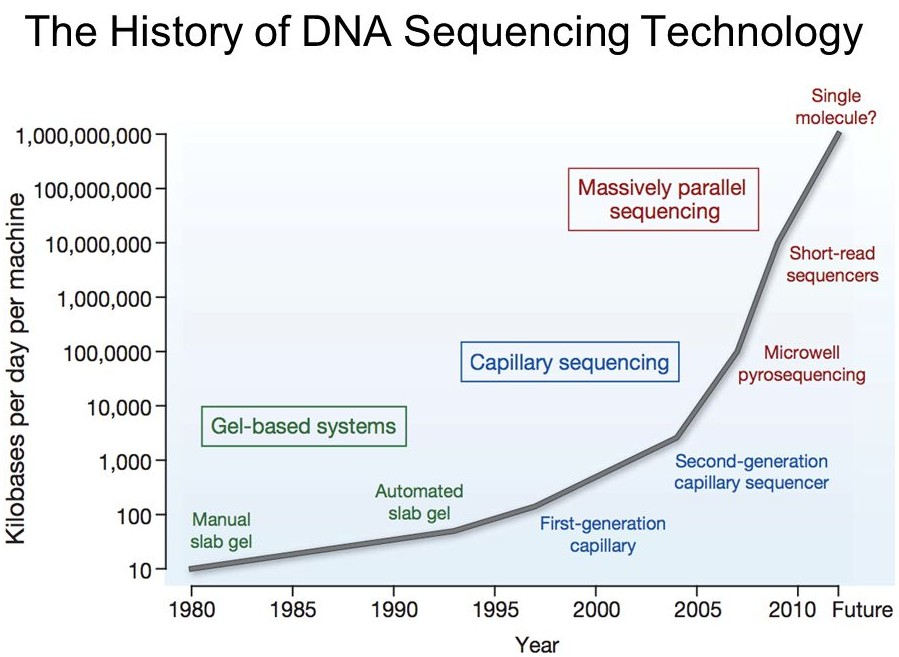
\includegraphics[width=0.85\textwidth]{c2.genomics/sequencing.history.01.jpg}
  \end{figure}
\end{frame}

\begin{frame}
  \frametitle{基因组学 | 测序 | 历史}
  \begin{figure}
    \centering
    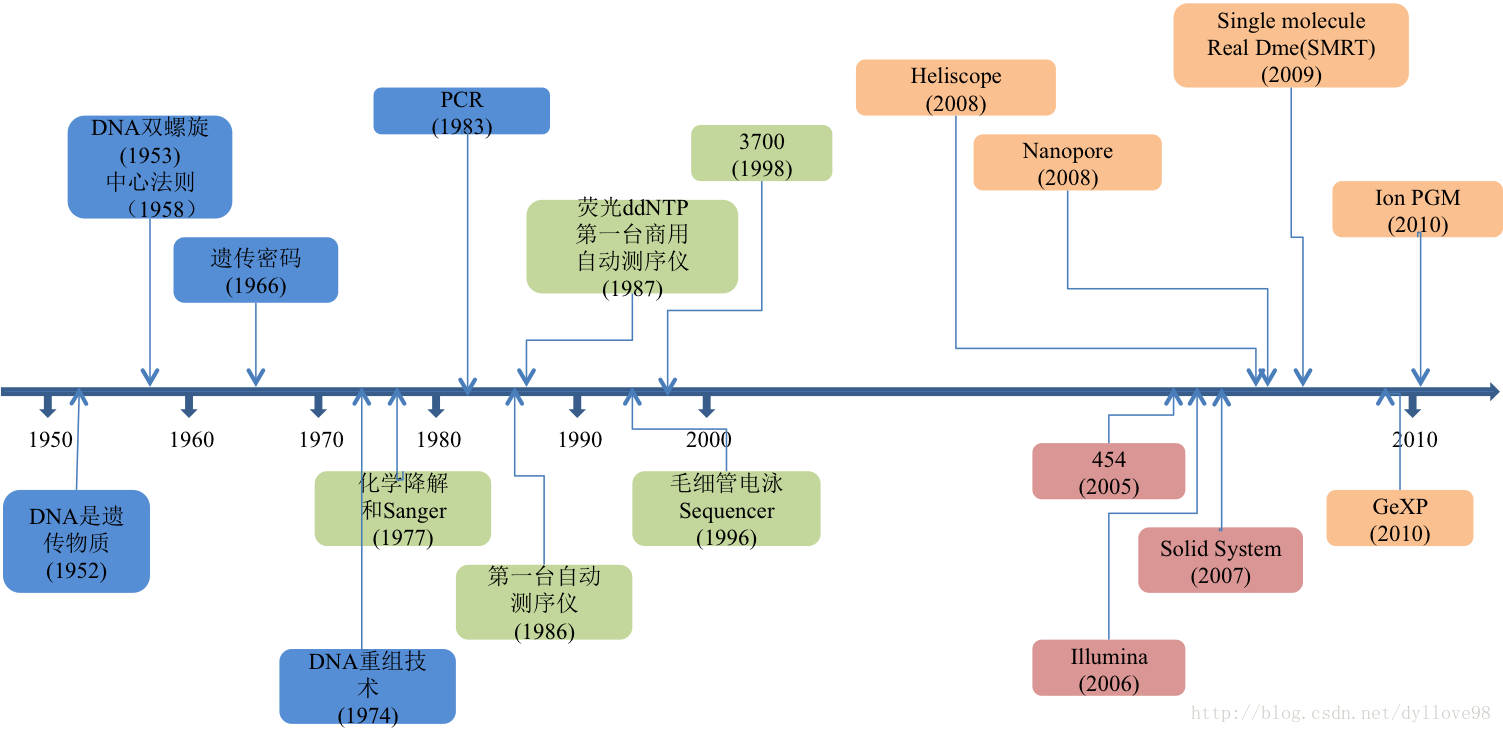
\includegraphics[width=0.9\textwidth]{c2.genomics/sequencing.timeline.01.png}
  \end{figure}
\end{frame}

\begin{frame}
  \frametitle{基因组学 | 测序 | 历史}
  \begin{figure}
    \centering
    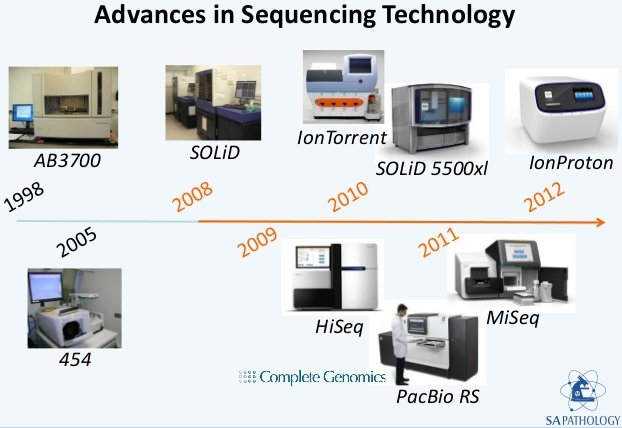
\includegraphics[width=0.9\textwidth]{c2.genomics/sequencing.timeline.03.jpg}
  \end{figure}
\end{frame}

\begin{frame}
  \frametitle{基因组学 | 测序 | 历史}
  \begin{figure}
    \centering
    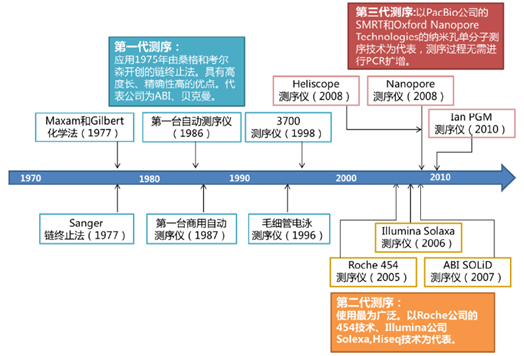
\includegraphics[width=0.9\textwidth]{c2.genomics/sequencing.timeline.02.png}
  \end{figure}
\end{frame}

\begin{frame}
  \frametitle{基因组学 | 测序 | 视频}
  \begin{figure}
    \centering
    
\includegraphics[width=6.5cm]{c2.dna.sequencing.png}
  \end{figure}
  \begin{center}
    \href{http://www.tudou.com/listplay/VL0WhYYzb_Y.html}{http://www.tudou.com/listplay/VL0WhYYzb\_Y.html}
  \end{center}
\end{frame}

\subsection{第一代测序技术}
\begin{frame}
  \frametitle{基因组学 | 测序 | 第一代 | 简介}
   \begin{itemize}
     \item 1975年,弗雷德里克·桑格(Frederick Sanger)和艾伦·库尔森(Alan Coulson),“加减测序法技术”;改进后为链终止法(chain termination method),即桑格测序法
     \item 1977年,哈佛大学的沃尔特·吉尔伯特(Walter Gilbert)和艾伦·马克萨姆(Allan Maxam),链降解,马克萨姆-吉尔伯特测序(Maxam-Gilbert法,又称化学测序法)
   \end{itemize} 
\end{frame}

\begin{frame}
  \frametitle{基因组学 | 测序 | 第一代 | 化学测序法}
  \begin{block}{化学测序法}
马克萨姆-吉尔伯特测序(Maxam-Gilbert sequencing)是一项由阿伦·马克萨姆与沃尔特·吉尔伯特于1976~1977年间开发的DNA测序方法。此项方法基于:对核碱基特异性地进行局部化学变性,接下来在变性核苷酸毗邻的位点处DNA骨架发生断裂。\\
\vspace{1em}
最初的桑格法须要在每次测序之前克隆得到单链DNA产物,因此马克萨姆-吉尔伯特测序法发表后迅速得到了推广,因为被纯化的DNA可被直接使用。然而,随着链终止法的改良,马克萨姆-吉尔伯特测序逐渐失宠,这是由于:技术复杂性阻碍其成为标准分子生物学套装使用、大量使用危险药品以及难于扩大规模。
  \end{block}
\end{frame}

\begin{frame}
  \frametitle{基因组学 | 测序 | 第一代 | 化学测序法}
  \begin{figure}
    \centering
    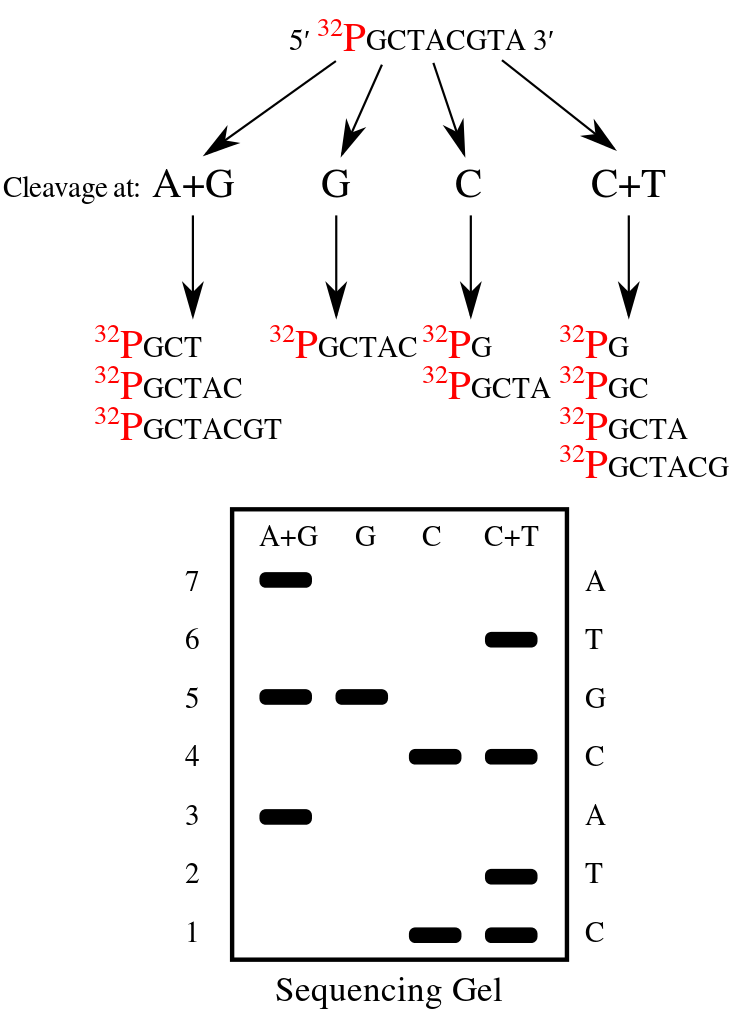
\includegraphics[width=0.48\textwidth]{c2.genomics/sequencing.mg.01.png}
  \end{figure}
\end{frame}

\begin{frame}
  \frametitle{基因组学 | 测序 | 第一代 | \textcolor{red}{桑格测序法}}
  \begin{block}{桑格测序法}
Sanger(桑格)双脱氧链终止法是弗雷德里克·桑格(Frederick Sanger)于1975年发明的。测序过程需要先做一个聚合酶连锁反应(PCR)。PCR过程中,双脱氧核糖核苷酸可能随机的被加入到正在合成中的DNA片段里。由于双脱氧核糖核苷酸少了一个氧原子,一旦它被加入到DNA链上,这个DNA链就不能继续增加长度。最终的结果是获得所有可能获得的、不同长度的DNA片段。\\
\vspace{1em}
目前最普遍最先进的方法,是将双脱氧核糖核苷酸进行不同荧光标记。将PCR反应获得的总DNA通过毛细管电泳分离,跑到最末端的DNA就可以在激光的作用下发出荧光。由于ddATP, ddGTP, ddCTP, ddTTP(4种双脱氧核糖核苷酸)荧光标记不同,计算机可以自动根据颜色判断该位置上碱基究竟是A,T,G,C中的哪一个。 
  \end{block}
\end{frame}

\begin{frame}
  \frametitle{基因组学 | 测序 | 第一代 | 桑格测序法}
  \begin{block}{原理}
双脱氧链终止法采用DNA复制原理。Sanger测序反应体系中包括目标DNA片断、脱氧三磷酸核苷酸(dNTP)、双脱氧三磷酸核苷酸(ddNTP)、测序引物及DNA聚合酶等。\\
\vspace{1em}
测序反应的核心就是其使用的ddNTP:由于缺少3'-OH基团,不具有与另一个dNTP连接形成磷酸二酯键的能力,这些ddNTP可用来中止DNA链的延伸。此外,这些ddNTP上连接有放射性同位素或荧光标记基团,因此可以被自动化的仪器或凝胶成像系统所检测到。
  \end{block}
\end{frame}

\begin{frame}
  \frametitle{基因组学 | 测序 | 第一代 | 桑格测序法}
  \begin{block}{概述}
    每个反应含有所有四种脱氧三磷酸核苷酸(dNTP)使之扩增,并混入限量的一种不同的双脱氧三磷酸核苷酸(ddNTP)使之终止。由于ddNTP缺乏延伸所需要的3'-OH基团,使延长的寡聚核苷酸选择性地在G、A、T或C处终止,终止点由反应中相应的ddNTP而定。\\
\vspace{1em}
每一种dNTPs和ddNTPs的相对浓度可以调整,使反应得到一组长几个至千以上个、相差一个碱基的一系列片断。它们具有共同的起始点,但终止在不同的核苷酸上,可通过高分辨率变性凝胶电泳分离大小不同的片段,凝胶处理后可用X-光胶片放射自显影或非同位素标记进行检测。
  \end{block}
\end{frame}

\begin{frame}
  \frametitle{基因组学 | 测序 | 第一代 | 桑格测序法}
  \begin{block}{优势}
    \begin{itemize}
      \item 最长可测定600-1000bp的DNA片断
      \item 对重复序列和多聚序列的处理较好
      \item 序列准确性高,高达99.999\%
      \item 测序的“黄金标准”
    \end{itemize}
  \end{block}
  \pause
  \begin{block}{缺点}
    \begin{itemize}
      \item 通量较低(在24h内可测定的DNA分子数一般不超过10,000个)
      \item 每碱基测序成本较高
      \item 不适合大规模平行测序
    \end{itemize}
  \end{block}
\end{frame}

\begin{frame}
  \frametitle{基因组学 | 测序 | 第一代 | 桑格测序法}
  \begin{figure}
    \centering
    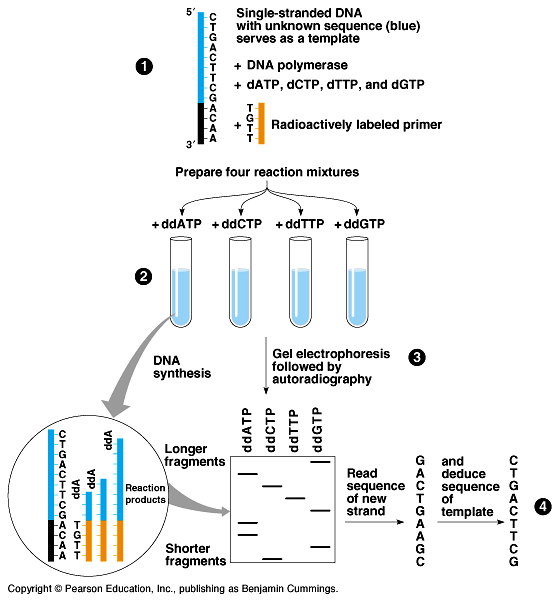
\includegraphics[width=0.6\textwidth]{c2.genomics/sequencing.sanger.01.png}
  \end{figure}
\end{frame}

\begin{frame}
  \frametitle{基因组学 | 测序 | 第一代 | 桑格测序法}
  \begin{figure}
    \centering
    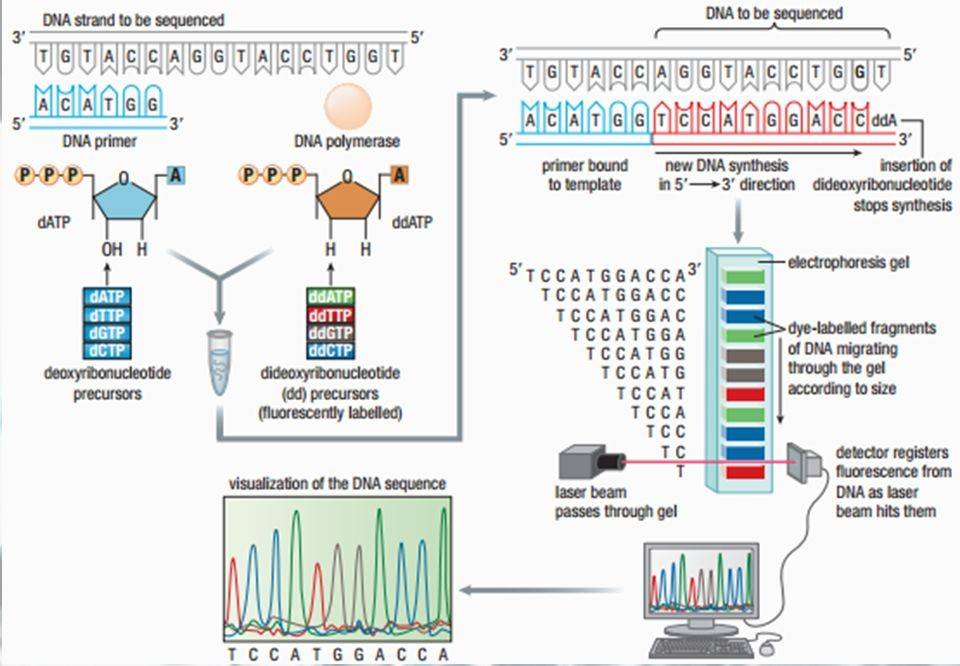
\includegraphics[width=0.9\textwidth]{c2.genomics/sequencing.sanger.04.jpg}
  \end{figure}
\end{frame}

\subsection{第二代测序技术}
\begin{frame}
  \frametitle{基因组学 | 测序 | 第二代 | 引言}
  \begin{block}{Reads}
    \begin{columns}
      \column{0.2\textwidth}
      \column{0.3\textwidth}
一个完美的人 \\ ,不是寻找一 \\ 眼光,欣赏那 \\ 爱,不是寻找 \\ 是学会用完美 \\  不完美的人。 \\
      \column{0.3\textwidth}
是寻找一个完 \\ 的人,而是学 \\ 完美的眼光, \\ ,欣赏那个并 \\ 完美的人,而 \\ 那个并不完美  \\
      \column{0.2\textwidth}
    \end{columns}
  \end{block}
  \pause
  \pause
  \pause
  \pause
  \begin{block}{基因组}
    爱,不是寻找一个完美的人,而是学会用完美的眼光,欣赏那个并不完美的人。——《哈尔的移动城堡》
  \end{block}
\end{frame}

\begin{frame}
  \frametitle{基因组学 | 测序 | 第二代 | 引言}
  \begin{block}{Reads}
    \begin{columns}
      \column{0.2\textwidth}
      \column{0.3\textwidth}
      who you are \\ are, but \\ I love you \\ not for who \\ am with you \\ who I am \\
      \column{0.3\textwidth}
      love you not \\ but for who \\ you not for \\ for who I \\ with you. \\ you are, \\
      \column{0.2\textwidth}
    \end{columns}
  \end{block}
  \pause
  \pause
  \pause
  \pause
  \begin{block}{基因组}
    I love you not for who you are, but for who I am with you. ——《剪刀手爱德华》
  \end{block}
\end{frame}

\begin{frame}
  \frametitle{基因组学 | 测序 | 第二代 | 引言}
  \begin{figure}
    \centering
    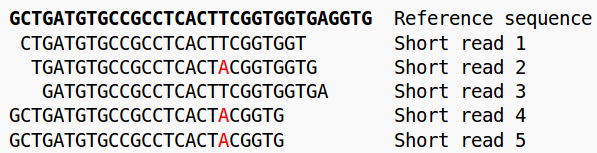
\includegraphics[width=\textwidth]{c2.genomics/ngs.reads.seq.01.png}
  \end{figure}
\end{frame}

\begin{frame}
  \frametitle{基因组学 | 测序 | 第二代 | 引言}
  \begin{figure}
    \centering
    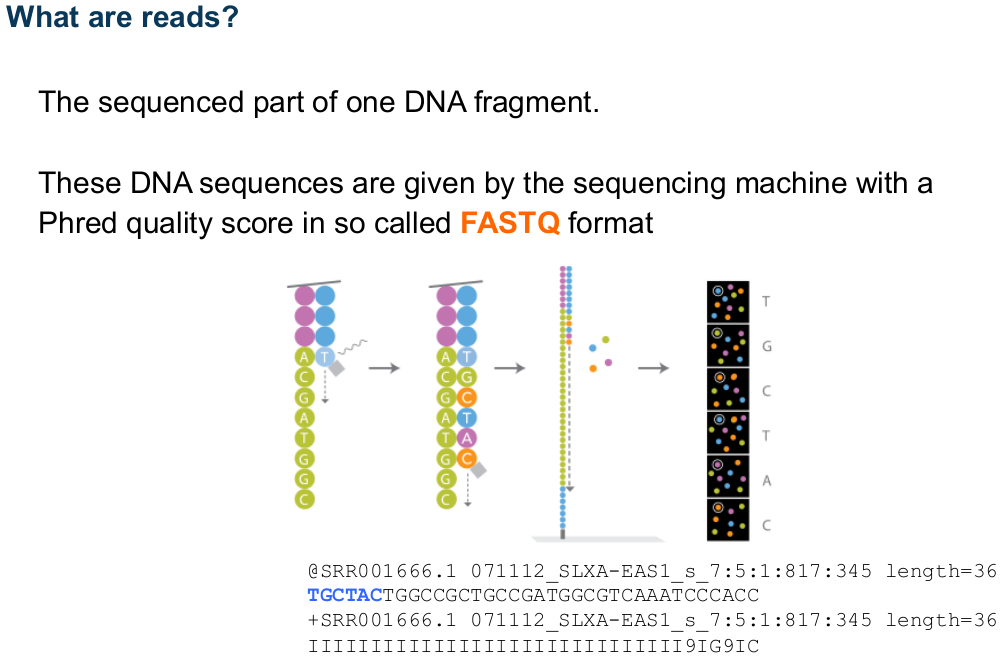
\includegraphics[width=\textwidth]{c2.genomics/ngs.reads.seq.02.png}
  \end{figure}
\end{frame}

\begin{frame}
  \frametitle{基因组学 | 测序 | 第二代 | 简介}
  \begin{block}{Roche公司的454技术}
  \begin{itemize}
    \item 1996年,波尔·尼伦和穆斯塔法·罗纳吉,焦磷酸测序(pyrosequencing)
    \item 2004/2005年,商业化测序仪
    \item 2009年,百万条、200-400bp
  \end{itemize}
  \end{block}
  \pause
  \begin{block}{Illumina公司的Solexa技术}
  \begin{itemize}
    \item 2006年,商业化测序仪
    \item 2009年,上亿条、50-100bp
  \end{itemize}
  \end{block}
  \pause
  \begin{block}{ABI公司的SOLiD技术}
  \begin{itemize}
    \item 2006/2007年,商业化测序仪
  \end{itemize}
  \end{block}
\end{frame}

\begin{frame}
  \frametitle{基因组学 | 测序 | 第二代 | \textcolor{red}{Roche/454}}
  \begin{block}{焦磷酸测序}
焦磷酸测序(pyrosequencing)是一种基于聚合原理的DNA测序方法,它依赖于核苷酸掺入中焦磷酸盐的释放,而非双脱氧三磷酸核苷酸参与的链终止反应。\\
\vspace{1em}
Pyrosequencing技术是由4种酶催化的同一反应体系中的酶级联化学发光反应。在每一轮测序中,只加入一种dNTP,若该dNTP与模板配对,聚合酶就可以将其掺入到引物链中并释放出等摩尔数的焦磷酸基团(PPi)。PPi可最终转化为可见光信号,并由PyrogramTM转化为一个峰值。每个峰值的高度与反应中掺入的核苷酸数目成正比。然后加入下一种dNTP,继续DNA链的合成。
  \end{block}
\end{frame}

\begin{frame}
  \frametitle{基因组学 | 测序 | 第二代 | Roche/454}
  \begin{figure}
    \centering
    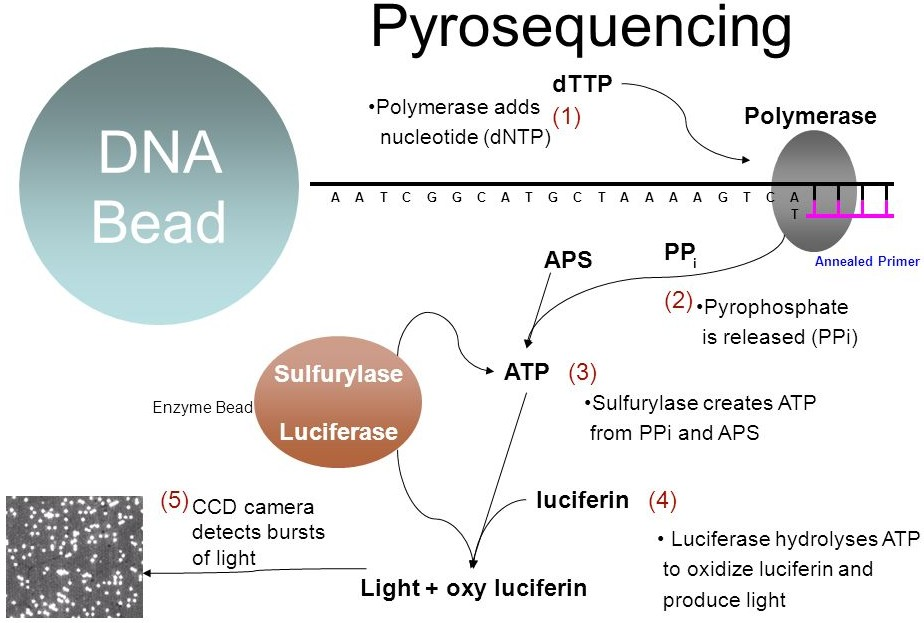
\includegraphics[width=0.9\textwidth]{c2.genomics/sequencing.pyro.02.jpg}
  \end{figure}
\end{frame}

\begin{frame}
  \frametitle{基因组学 | 测序 | 第二代 | \textcolor{red}{Roche/454}}
  \begin{block}{emPCR}
emPCR(乳液PCR)主要通过将水相PCR溶液(包含引物、聚合酶、核苷酸和待扩增DNA)与油混合,创建一种微小的悬浮水滴乳液。每个液滴都作为其自身PCR的“反应器”,从而创造了平行反应中的多个独立反应。\\
\vspace{1em}
emPCR(emulsion PCR)技术利用油包水(water-in-oil)结构作为PCR反应的微反应器,进行PCR扩增。emPCR最大的特点是可以形成数目庞大的独立反应空间以进行PCR扩增。其关键技术是“注水到油”,基本过程是在PCR反应前,将包含PCR所需反应成分的水溶液注入到高速旋转的油相表面,水溶液瞬间形成数以万计个被油相包裹的小液滴。这些小液滴就形成了PCR反应空间。
  \end{block}
\end{frame}

\begin{frame}
  \frametitle{基因组学 | 测序 | 第二代 | Roche/454}
  \begin{figure}
    \centering
    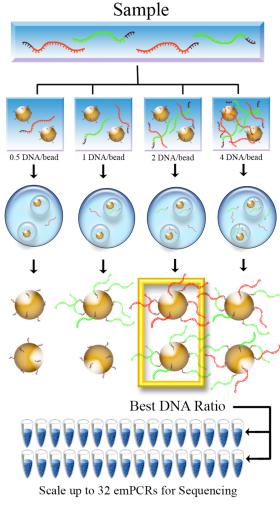
\includegraphics[width=0.36\textwidth]{c2.genomics/sequencing.empcr.01.jpg}
    \qquad
    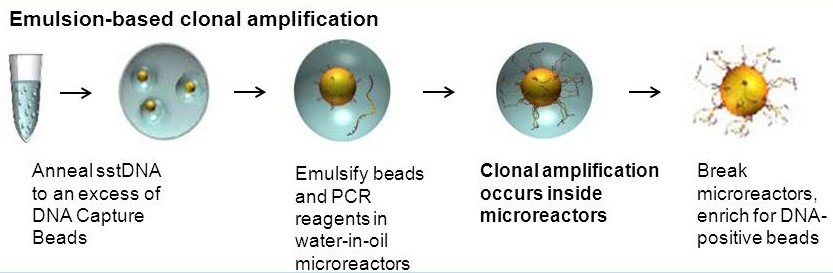
\includegraphics[angle=270,origin=r,width=0.18\textwidth]{c2.genomics/sequencing.empcr.05.jpg}
  \end{figure}
\end{frame}

\begin{frame}
  \frametitle{基因组学 | 测序 | 第二代 | \textcolor{red}{Roche/454}}
  \begin{block}{概述}
在测序时,使用了一种叫做“Pico TiterPlate”(PTP)的平板,它含有160多万个由光纤组成的孔,孔中载有化学发光反应所需的各种酶和底物。测序开始时,放置在四个单独的试剂瓶里的四种碱基,依照T、A、C、G的顺序依次循环进入PTP板,每次只进入一个碱基。如果发生碱基配对,就会释放一个焦磷酸。这个焦磷酸在各种酶的作用下,经过一个合成反应和一个化学发光反应,最终将荧光素氧化成氧化荧光素,同时释放出光信号。此反应释放出的光信号实时被仪器配置的高灵敏度CCD捕获到。有一个碱基和测序模板进行配对,就会捕获到一分子的光信号;由此一一对应,就可以准确、快速地确定待测模板的碱基序列。
  \end{block}
\end{frame}

% \begin{frame}
%   \frametitle{基因组学 | 测序 | 第二代 | Roche/454}
%   \begin{figure}
%     \centering
%     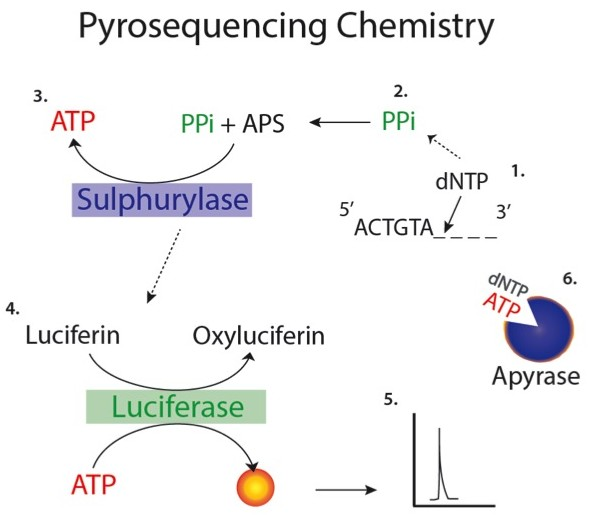
\includegraphics[width=0.7\textwidth]{c2.genomics/sequencing.pyro.01.jpg}
%   \end{figure}
% \end{frame}

\begin{frame}
  \frametitle{基因组学 | 测序 | 第二代 | Roche/454}
  \begin{figure}
    \centering
    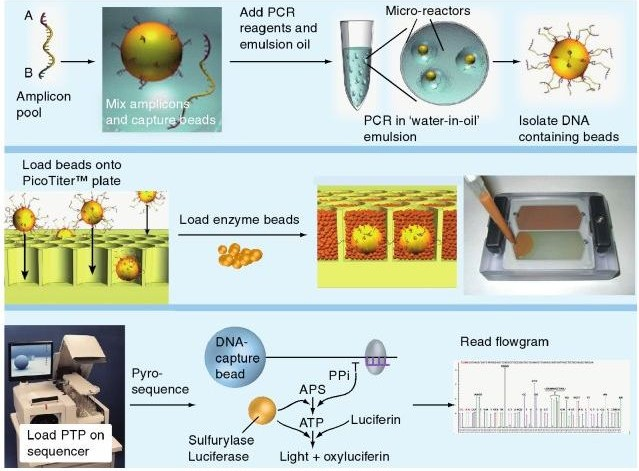
\includegraphics[width=0.9\textwidth]{c2.genomics/sequencing.454.01.jpg}
  \end{figure}
\end{frame}

\begin{frame}
  \frametitle{基因组学 | 测序 | 第二代 | Roche/454}
  \begin{block}{优点}
    \begin{itemize}
      \item 读长长,使得后继的序列拼接工作更加高效、准确
      \item 速度快,一个测序反应耗时10个小时,获得4-6亿个碱基对
      \item 特别适合从头拼接和宏基因组学应用,多用于新的细菌基因组
    \end{itemize}
  \end{block}
  \pause
  \begin{block}{缺点}
    \begin{itemize}
      \item 无法准确测量同聚物的长度,所以检测插入缺失突变的误差率高
      \item 通量小且费用高
      \item 对重测序来说太贵,不适合
    \end{itemize}
  \end{block}
\end{frame}

\begin{frame}
  \frametitle{基因组学 | 测序 | 第二代 | \textcolor{red}{Illumina/Solexa}}
  \begin{block}{桥式扩增}
桥式扩增(bridge amplification):随机打断的单链DNA片段通过两端接头与寡核苷酸的互补固定在芯片表面,形成桥形结构,之后以寡核苷酸为引物进行PCR扩增,得到单克隆的DNA簇群。
  \end{block}
\end{frame}

\begin{frame}
  \frametitle{基因组学 | 测序 | 第二代 | Illumina/Solexa}
  \begin{figure}
    \centering
    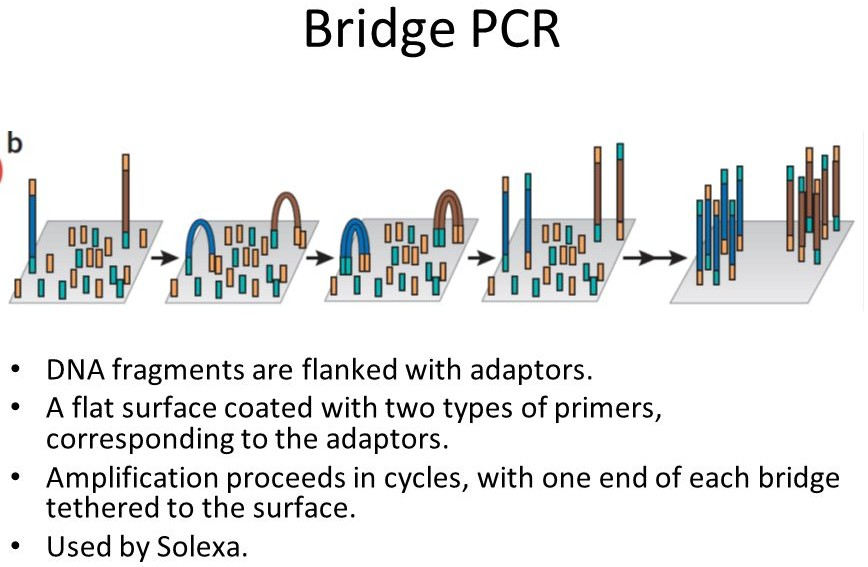
\includegraphics[width=0.9\textwidth]{c2.genomics/sequencing.bridge.01.jpg}
  \end{figure}
\end{frame}

\begin{frame}
  \frametitle{基因组学 | 测序 | 第二代 | Illumina/Solexa}
  \begin{figure}
    \centering
    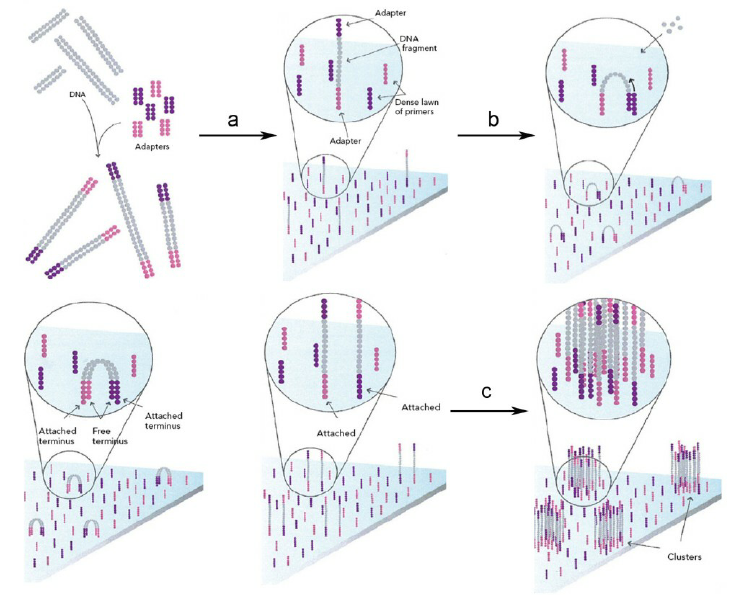
\includegraphics[width=0.8\textwidth]{c2.genomics/sequencing.bridge.02.png}
  \end{figure}
\end{frame}

\begin{frame}
  \frametitle{基因组学 | 测序 | 第二代 | \textcolor{red}{Illumina/Solexa}}
  \begin{block}{边合成边测序}
边合成边测序(sequencing by synthesis,SBS):以DNA单链为模板,在合成互补链的时候,利用带荧光标记的dNTP发出不同的荧光来确定碱基类型。
  \end{block}
\end{frame}

\begin{frame}
  \frametitle{基因组学 | 测序 | 第二代 | Illumina/Solexa}
  \begin{figure}
    \centering
    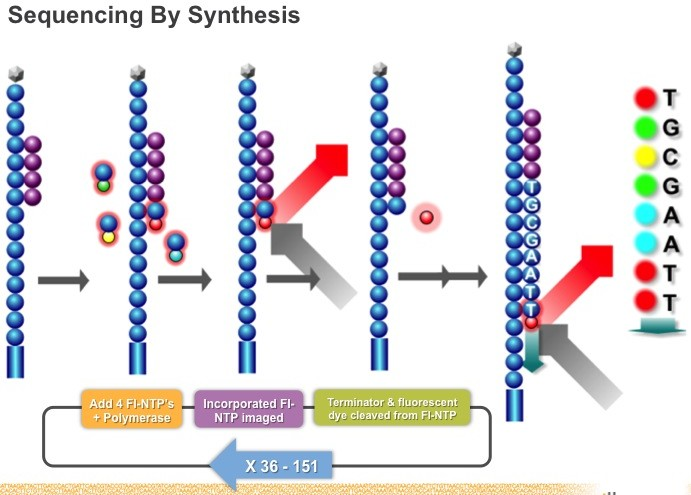
\includegraphics[width=0.9\textwidth]{c2.genomics/sequencing.sbs.01.jpg}
  \end{figure}
\end{frame}

\begin{frame}
  \frametitle{基因组学 | 测序 | 第二代 | Illumina/Solexa}
  \begin{figure}
    \centering
    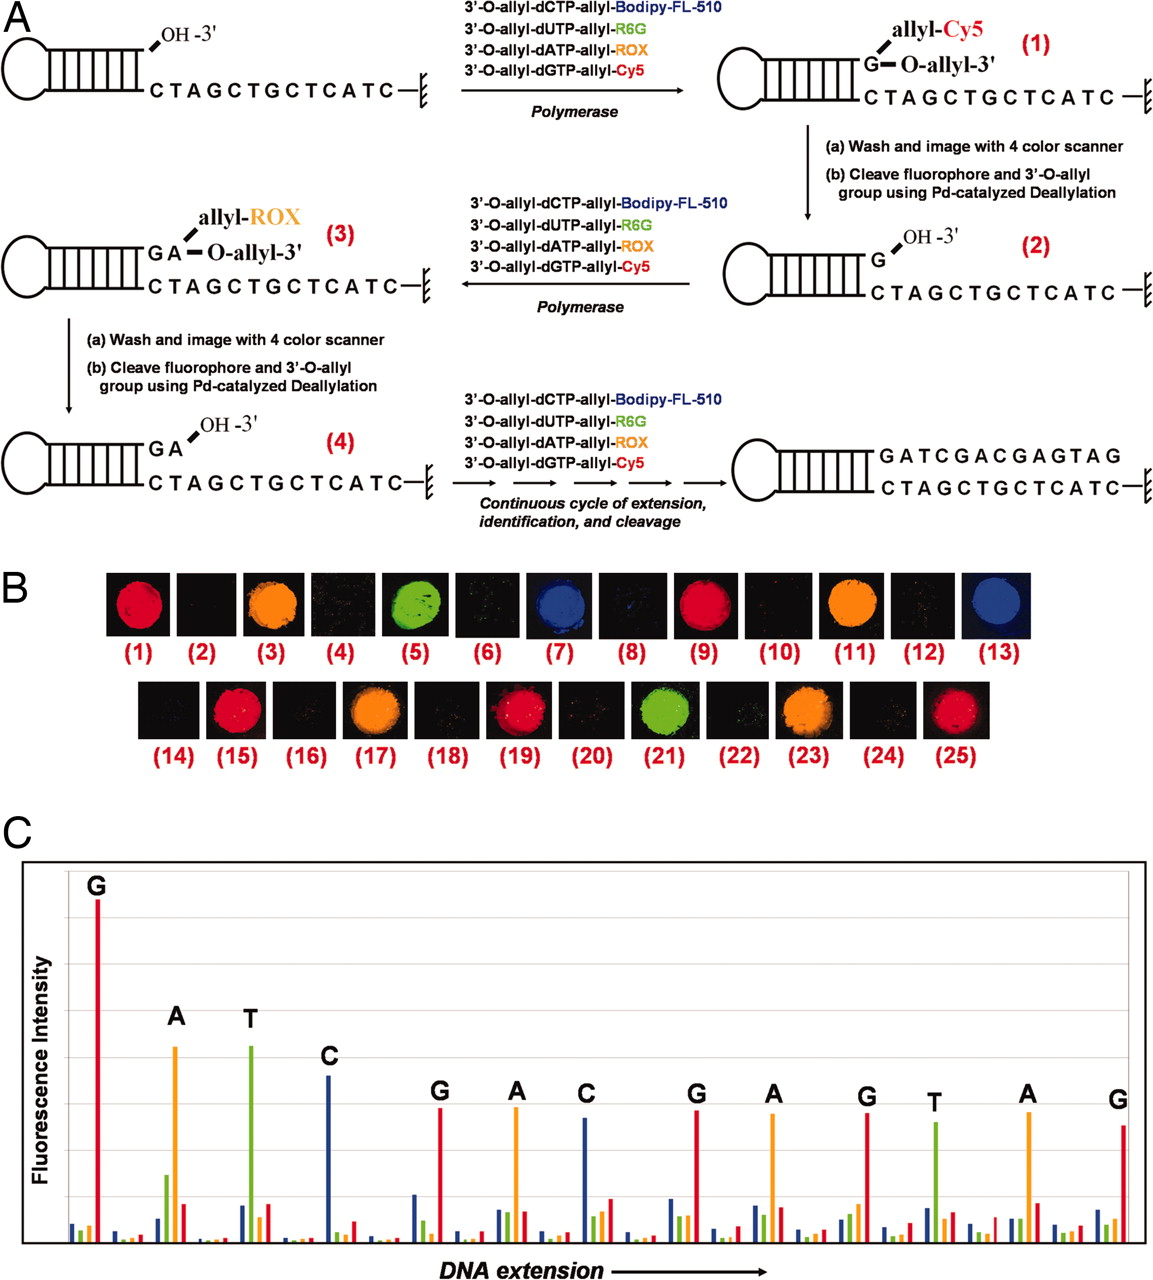
\includegraphics[width=0.59\textwidth]{c2.genomics/sequencing.sbs.04.jpg}
  \end{figure}
\end{frame}

\begin{frame}
  \frametitle{基因组学 | 测序 | 第二代 | \textcolor{red}{Illumina/Solexa}}
  \begin{block}{概述}
这种测序技术通过将基因组DNA的随机片断附着到光学透明的表面,这些DNA片断通过延长和桥梁扩增,形成了具有数以亿计cluster的Flowcell,每个cluster具有约1000拷贝的相同DNA模板,然后用4种末端被封闭的不同荧光标记的碱基进行边合成边测序。这种新方法确保了高精确度和真实的一个碱基接一个碱基的测序,排除了序列方面的特殊错误,能够测序同聚物和重复序列。
  \end{block}
\end{frame}

\begin{frame}
  \frametitle{基因组学 | 测序 | 第二代 | Illumina/Solexa}
  \begin{figure}
    \centering
    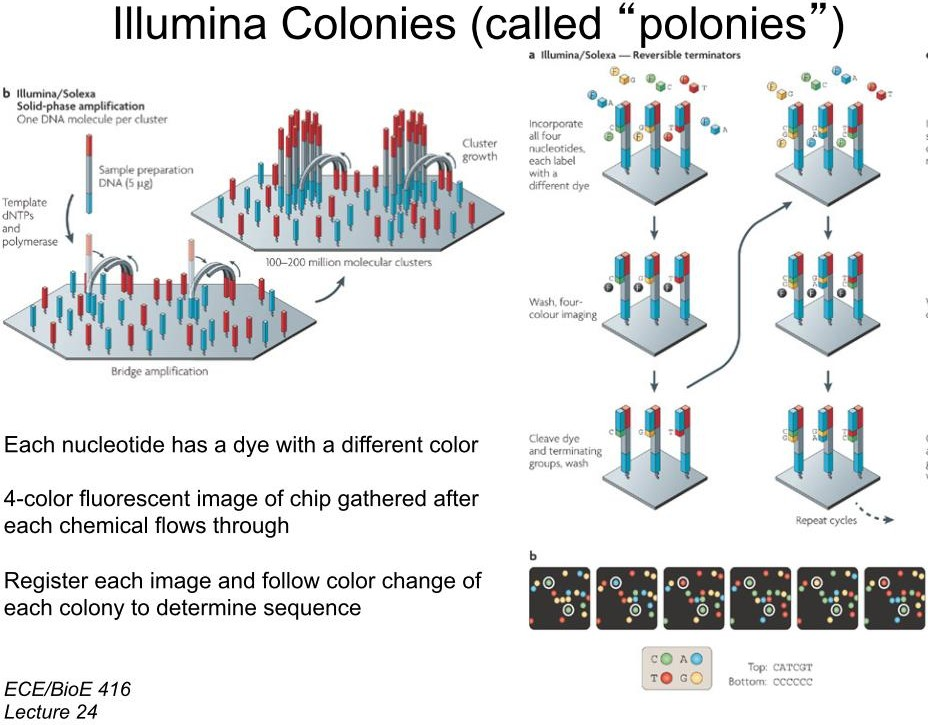
\includegraphics[width=0.82\textwidth]{c2.genomics/sequencing.ill.05.jpg}
  \end{figure}
\end{frame}

\begin{frame}
  \frametitle{基因组学 | 测序 | 第二代 | Illumina/Solexa}
  \begin{figure}
    \centering
    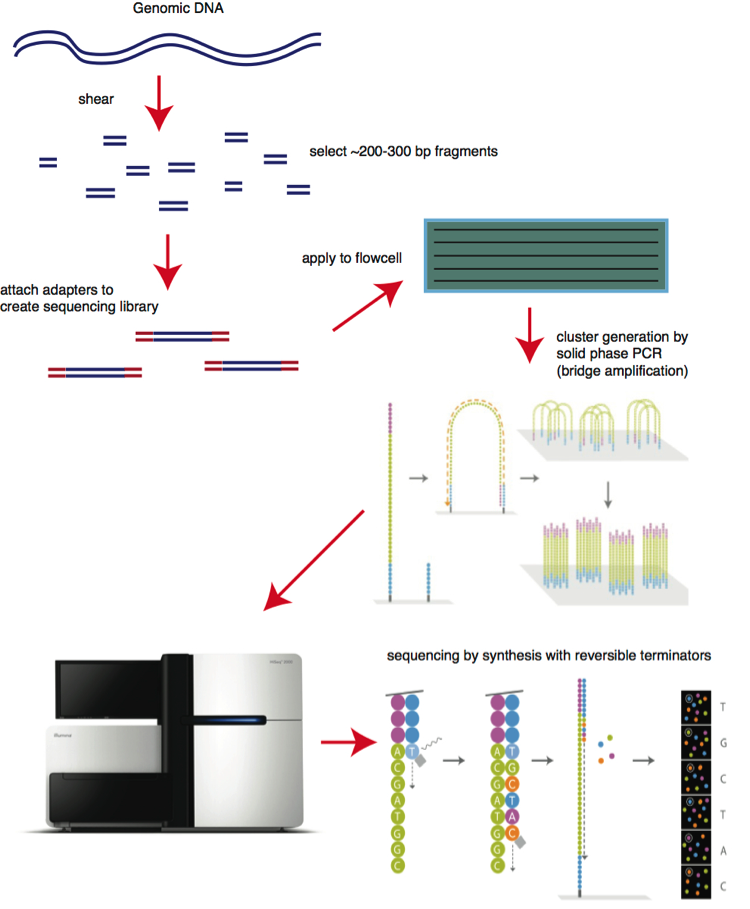
\includegraphics[width=0.52\textwidth]{c2.genomics/sequencing.ill.01.png}
  \end{figure}
\end{frame}

\begin{frame}
  \frametitle{基因组学 | 测序 | 第二代 | Illumina/Solexa}
  \begin{block}{优点}
    \begin{itemize}
      \item 通量大
      \item 测序方式灵活
      \item 分析软件多样化
    \end{itemize}
  \end{block}
  \pause
  \begin{block}{缺点}
    \begin{itemize}
      \item 样本制备过程复杂
      \item 样本要求相对较高
    \end{itemize}
  \end{block}
\end{frame}

\begin{frame}
  \frametitle{基因组学 | 测序 | 第二代 | \textcolor{red}{ABI/SOLiD}}
  \begin{block}{边连接边测序}
边连接边测序(sequencing by ligation),基于连接酶法,即利用DNA连接酶在连接过程之中测序。  
  \end{block}
\end{frame}

\begin{frame}
  \frametitle{基因组学 | 测序 | 第二代 | ABI/SOLiD}
  \begin{figure}
    \centering
    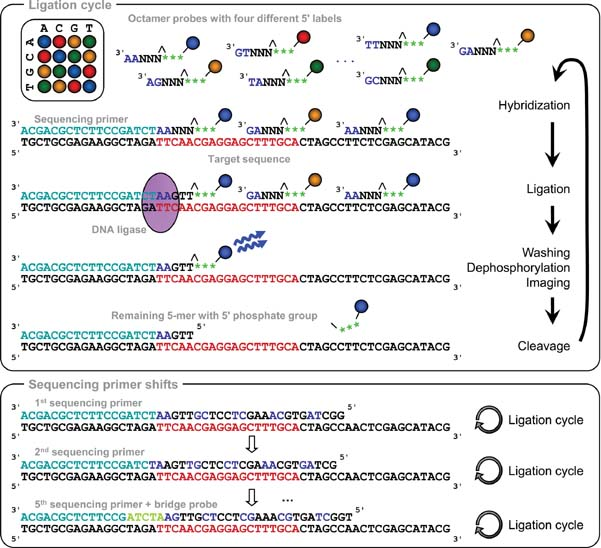
\includegraphics[width=0.7\textwidth]{c2.genomics/sequencing.sbl.01.jpg}
  \end{figure}
\end{frame}

\begin{frame}
  \frametitle{基因组学 | 测序 | 第二代 | \textcolor{red}{ABI/SOLiD}}
  \begin{block}{概述}
SOLiD连接反应的底物是8碱基单链荧光探针混合物(3'-XXnnnzzz-5'),其中第1和第2位碱基(XX)上的碱基是确定的,并根据种类的不同在6-8位(zzz)上加上CY5、Texas Red、CY3、6-FAM四种不同的荧光标记。这是SOLiD的独特测序法,两个碱基确定一个荧光信号,相当于一次能决定两个碱基,因此也称为两碱基测序法。当荧光探针能够与DNA模板链配对而连接上时,就会发出代表第1、2位碱基的荧光信号。在记录下荧光信号后,通过化学方法在第5和第6位碱基之间进行切割,这样就能移除荧光信号,以便进行下一个位置的测序。这种测序方法每次测序的位置都相差5位:即第一次是第1、2位,第二次是第6、7位……在测到末尾后,要将新合成的链变性,洗脱。接着用引物n-1进行第二轮测序。引物n-1与引物n的区别是,二者在与接头配对的位置上相差一个碱基。也即是,通过引物n-1在引物n的基础上将测序位置往3'端移动一个碱基位置,因而就能测定第0、1位和第5、6位……第二轮测序完成,依此类推,直至第五轮测序,最终可以完成所有位置的碱基测序,并且每个位置的碱基均被检测了两次。
  \end{block}
\end{frame}

\begin{frame}
  \frametitle{基因组学 | 测序 | 第二代 | ABI/SOLiD}
  \begin{figure}
    \centering
    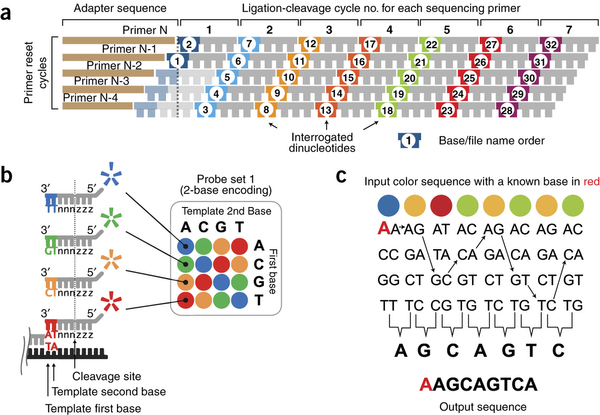
\includegraphics[width=0.9\textwidth]{c2.genomics/sequencing.sbl.02.jpg}
  \end{figure}
\end{frame}

% \begin{frame}
%   \frametitle{基因组学 | 测序 | 第二代 | ABI/SOLiD}
%   \begin{figure}
%     \centering
%     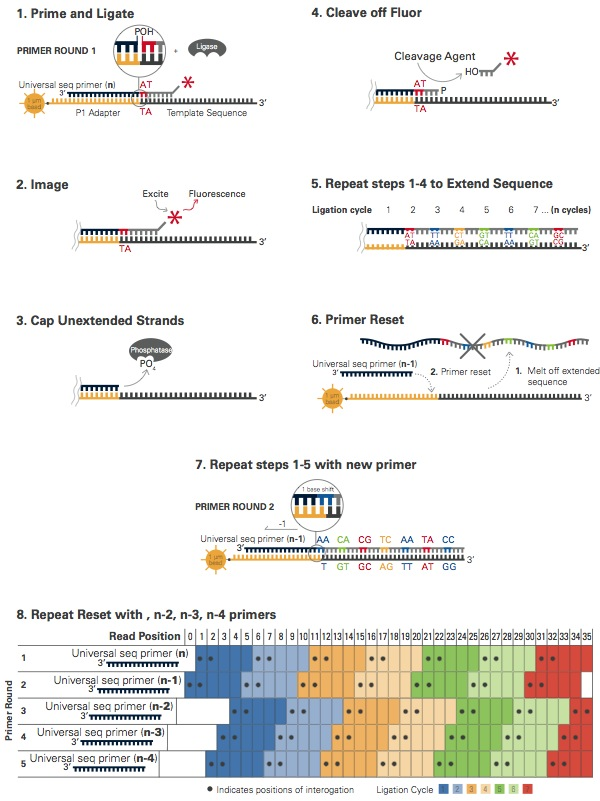
\includegraphics[width=0.48\textwidth]{c2.genomics/sequencing.sbl.03.jpg}
%   \end{figure}
% \end{frame}

\begin{frame}
  \frametitle{基因组学 | 测序 | 第二代 | ABI/SOLiD}
  \begin{figure}
    \centering
    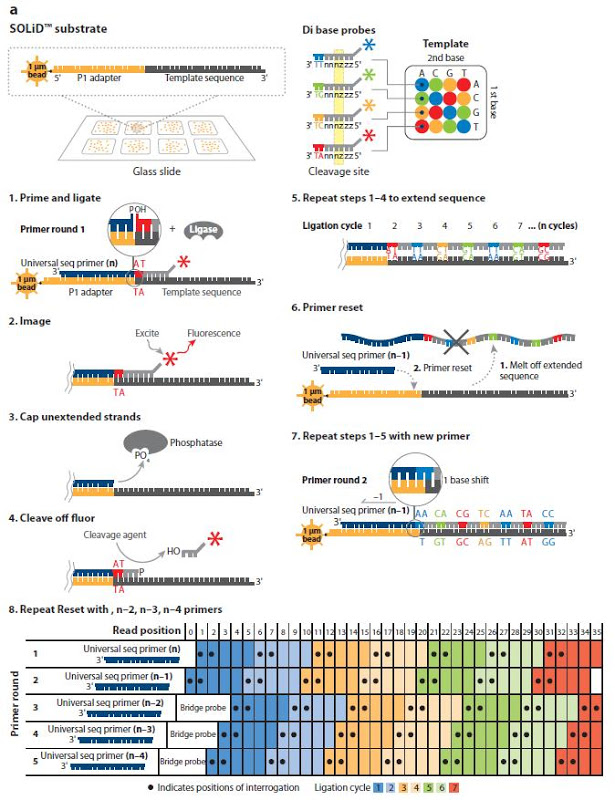
\includegraphics[width=0.48\textwidth]{c2.genomics/sequencing.solid.02.jpg}
  \end{figure}
\end{frame}

\begin{frame}
  \frametitle{基因组学 | 测序 | 第二代 | ABI/SOLiD}
  \begin{figure}
    \centering
    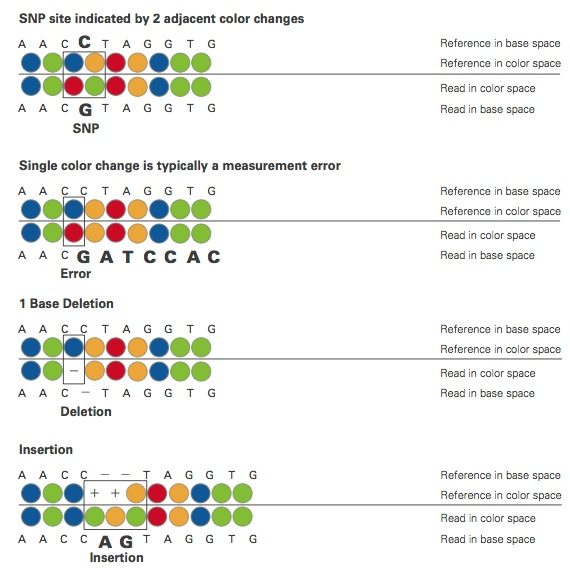
\includegraphics[width=0.62\textwidth]{c2.genomics/sequencing.sbl.04.jpg}
  \end{figure}
\end{frame}

\begin{frame}
  \frametitle{基因组学 | 测序 | 第二代 | ABI/SOLiD}
  \begin{figure}
    \centering
    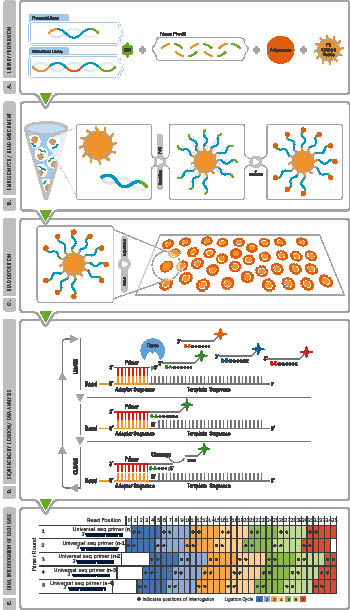
\includegraphics[width=0.38\textwidth]{c2.genomics/sequencing.solid.01.jpg}
  \end{figure}
\end{frame}

\begin{frame}
  \frametitle{基因组学 | 测序 | 第二代 | ABI/SOLiD}
  \begin{block}{优点}
    \begin{itemize}
      \item 高准确性,每个DNA碱基检测2次,增加了序列读取的准确性
    \end{itemize}
  \end{block}
  \pause
  \begin{block}{缺点}
    \begin{itemize}
      \item 运行时间长,检测碱基替换突变的误差率高
    \end{itemize}
  \end{block}
\end{frame}

\begin{frame}
  \frametitle{基因组学 | 测序 | 第2.5代 | 离子半导体测序}
  \begin{block}{概述}
    Ion Torrent(Ion semiconductor sequencing)是一种基于半导体芯片的新一代革命性测序技术,通过检测H+信号的变化来获得序列碱基信息。该技术使用了一种布满小孔的高密度半导体芯片,一个小孔就是一个测序反应池,芯片置于一个离子敏感层和离子感受器之上。当DNA聚合酶把核苷酸聚合到延伸中的DNA链上时,会释放出一个氢离子,反应池中的pH发生改变,位于池下的离子感受器感受到H+离子信号,H+离子信号再直接转化为数字信号,从而读出DNA序列。
  \end{block}
\end{frame}

\begin{frame}
  \frametitle{基因组学 | 测序 | 第2.5代 | 离子半导体测序}
  \begin{figure}
    \centering
    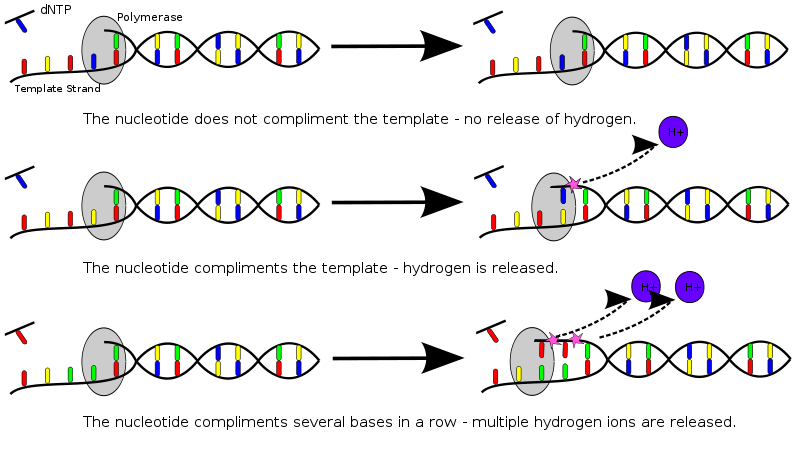
\includegraphics[width=0.9\textwidth]{c2.genomics/sequencing.ion.01.png}
  \end{figure}
\end{frame}

% \begin{frame}
%   \frametitle{基因组学 | 测序 | 第2.5代 | 离子半导体测序}
%   \begin{figure}
%     \centering
%     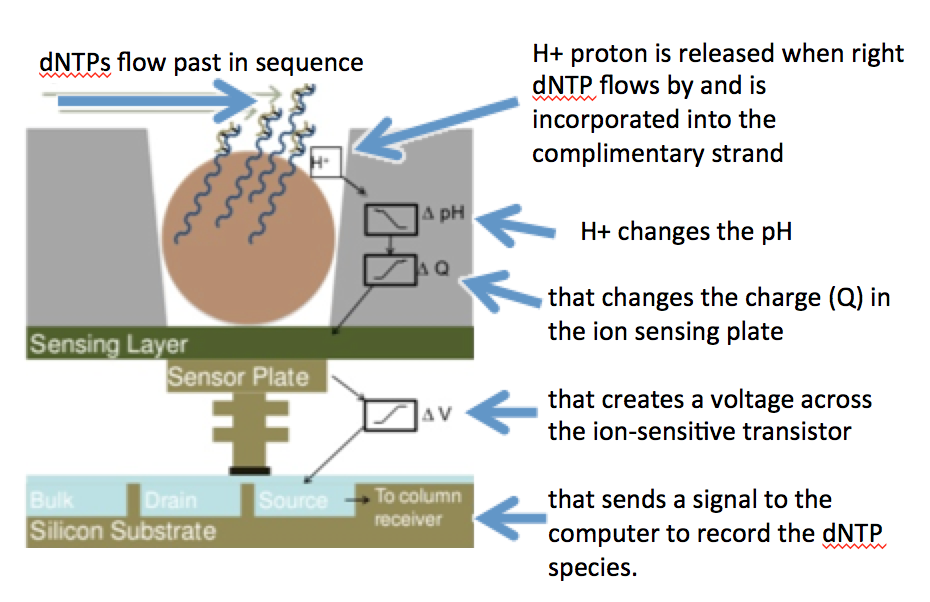
\includegraphics[width=0.9\textwidth]{c2.genomics/sequencing.ion.02.png}
%   \end{figure}
% \end{frame}

\begin{frame}
  \frametitle{基因组学 | 测序 | 第2.5代 | 离子半导体测序}
  \begin{figure}
    \centering
    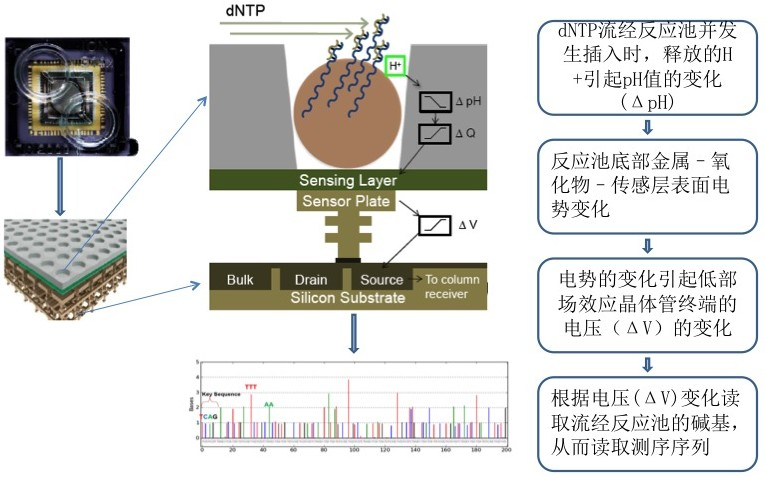
\includegraphics[width=0.9\textwidth]{c2.genomics/sequencing.ion.07.jpg}
  \end{figure}
\end{frame}

\begin{frame}
  \frametitle{基因组学 | 测序 | 第2.5代 | 离子半导体测序}
  \begin{figure}
    \centering
    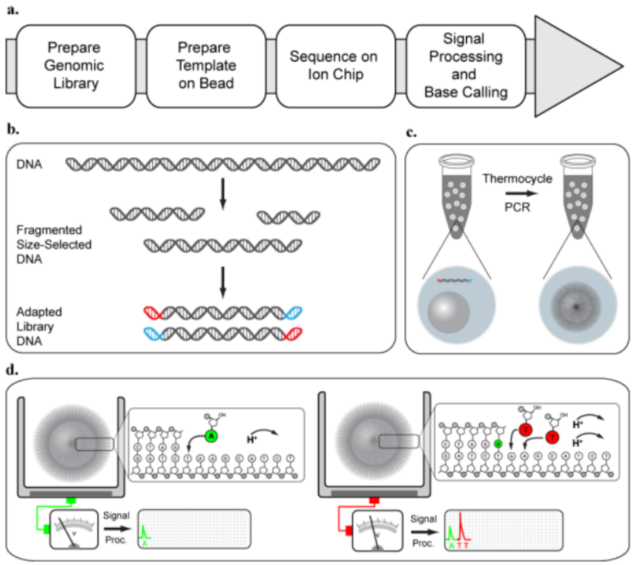
\includegraphics[width=0.7\textwidth]{c2.genomics/sequencing.ion.03.png}
  \end{figure}
\end{frame}

\begin{frame}
  \frametitle{基因组学 | 测序 | 第2.5代 | 离子半导体测序}
  \begin{figure}
    \centering
    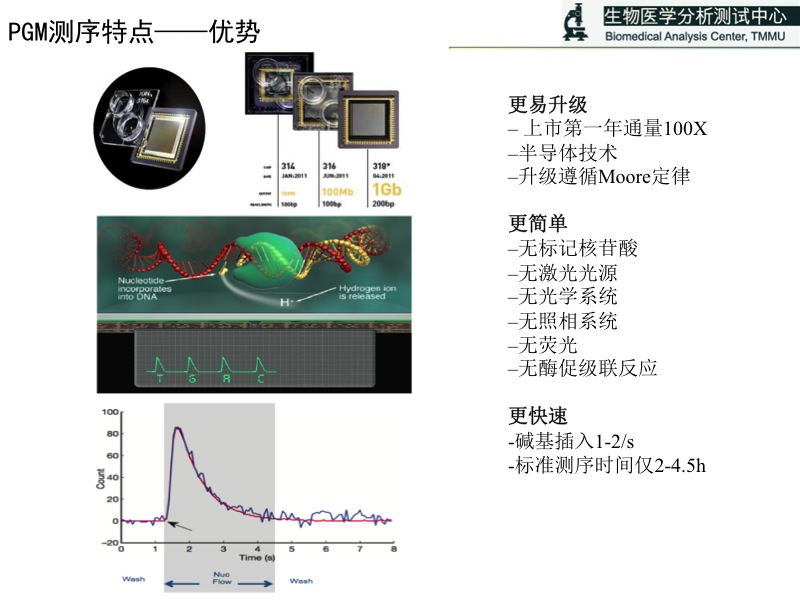
\includegraphics[width=0.85\textwidth]{c2.genomics/sequencing.ion.08.jpg}
  \end{figure}
\end{frame}

\begin{frame}
  \frametitle{基因组学 | 测序 | 第2.5代 | 离子半导体测序}
  \begin{block}{优缺点}
Ion Torrent相比于其他测序技术来说,不需要昂贵的物理成像等设备,因此,成本相对来说会低,体积也会比较小,同时操作也要更为简单,速度也相当快速,除了2天文库制作时间,整个上机测序可在2-3.5小时内完成,不过整个芯片的通量并不高,目前是10G左右,但非常适合小基因组和外显子验证的测序。\\
\vspace{1em}
Ion Torrent的化学测序原理自然简单,无修饰的核苷酸、无激光器或光学检测设备,因而可达到极小的测序偏差和出色的测序覆盖均衡度。
  \end{block}
\end{frame}

% \begin{frame}
%   \frametitle{基因组学 | 测序 | 第2.5代 | 离子半导体测序}
%   \begin{figure}
%     \centering
%     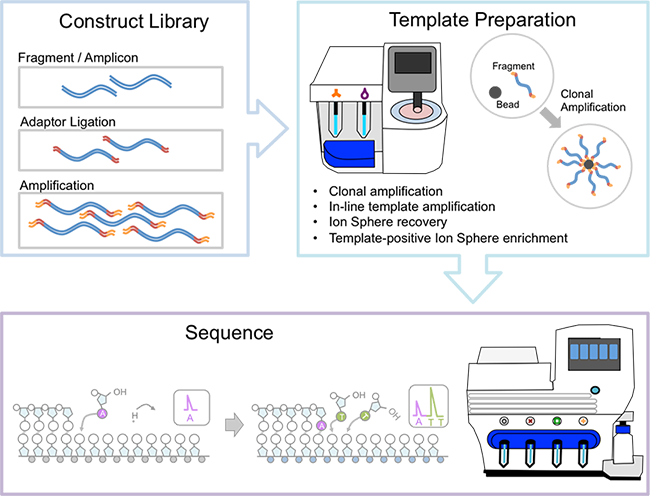
\includegraphics[width=0.8\textwidth]{c2.genomics/sequencing.ion.04.png}
%   \end{figure}
% \end{frame}


\begin{frame}
  \frametitle{基因组学 | 测序 | 第二代 | 比较}
  \begin{figure}
    \centering
    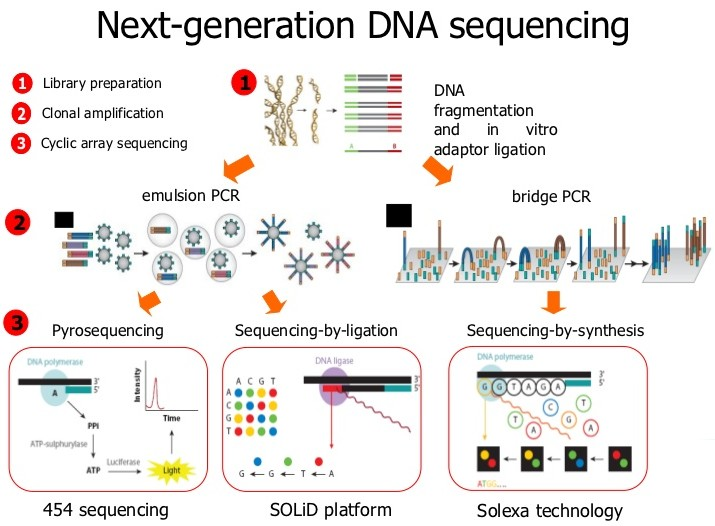
\includegraphics[width=0.88\textwidth]{c2.genomics/sequencing.ngs.01.jpg}
  \end{figure}
\end{frame}

\begin{frame}
  \frametitle{基因组学 | 测序 | 第二代 | 比较}
  \begin{figure}
    \centering
    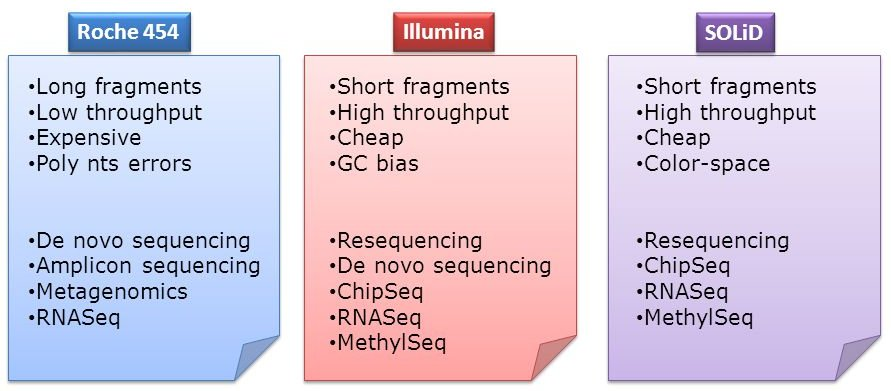
\includegraphics[width=0.9\textwidth]{c2.genomics/sequencing.compare.00.jpg}
  \end{figure}
\end{frame}

\subsection{第三代测序技术}
\begin{frame}
  \frametitle{基因组学 | 测序 | 第三代 | 简介}
  \begin{block}{单分子测序}
测序过程无需进行PCR扩增。 
  \end{block}
\end{frame}

\begin{frame}
  \frametitle{基因组学 | 测序 | 第三代 | tSMS}
  \begin{block}{概述}
真正的单分子测序(Helicos True Single Molecule Sequencing)。待测DNA被随机打断成小片段,在每个小片段(~200bp)的末端加上poly-dA,并于玻璃芯片上随机固定多个poly-dT引物,其末端皆带有荧光标记,以利于精确定位。首先,将小片段DNA模板与检测芯片上的poly-dT引物进行杂交并精确定位,然后逐一加入荧光标记的末端终止子。这个终止子与Illumina的终止子可不一样,不是四色的,是单色的,也就是说所有终止子都标有同一种染料。在掺入了单个荧光标记的核苷酸后,洗涤,单色成像,之后切开荧光染料和抑制基团,洗涤,加帽,允许下一个核苷酸的掺入。通过掺入、检测和切除的反复循环,即可实时读取大量序列。最后以软件系统辅助,可分析出完整的核酸序列。
  \end{block}
\end{frame}

\begin{frame}
  \frametitle{基因组学 | 测序 | 第三代 | tSMS}
  \begin{figure}
    \centering
    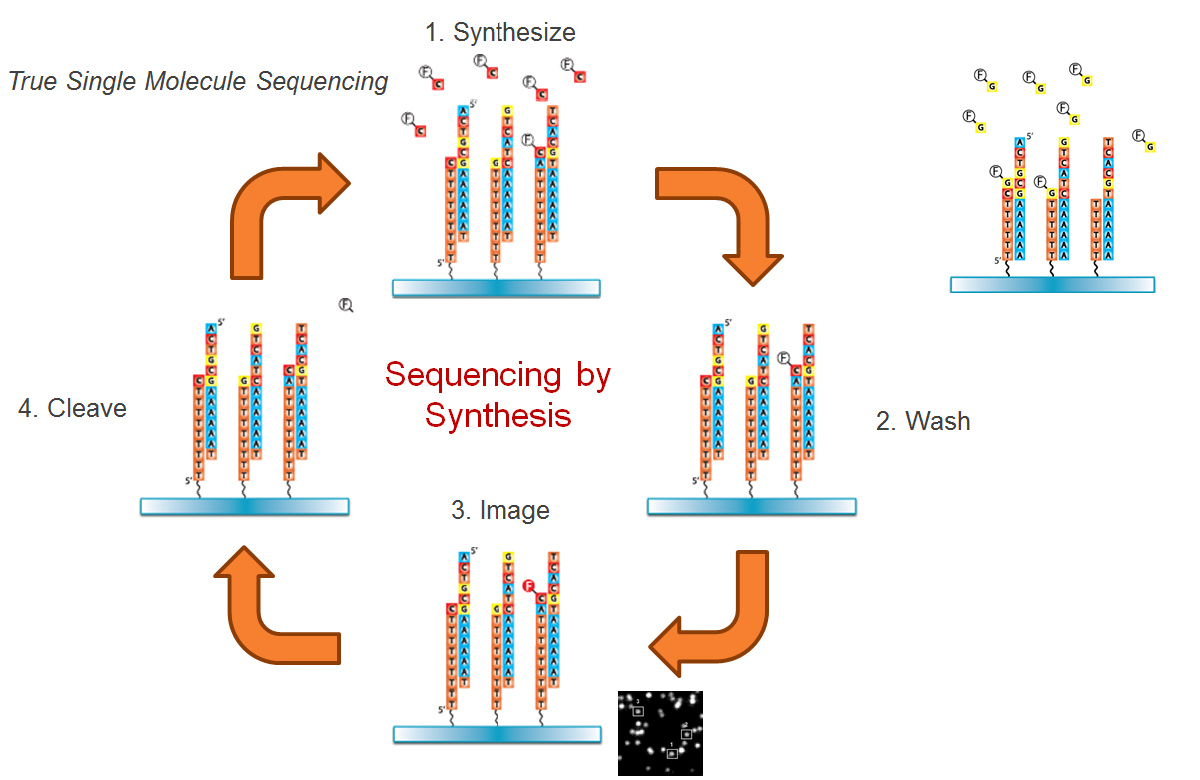
\includegraphics[width=0.9\textwidth]{c2.genomics/sequencing.sms.01.jpg}
  \end{figure}
\end{frame}

\begin{frame}
  \frametitle{基因组学 | 测序 | 第三代 | tSMS}
  \begin{figure}
    \centering
    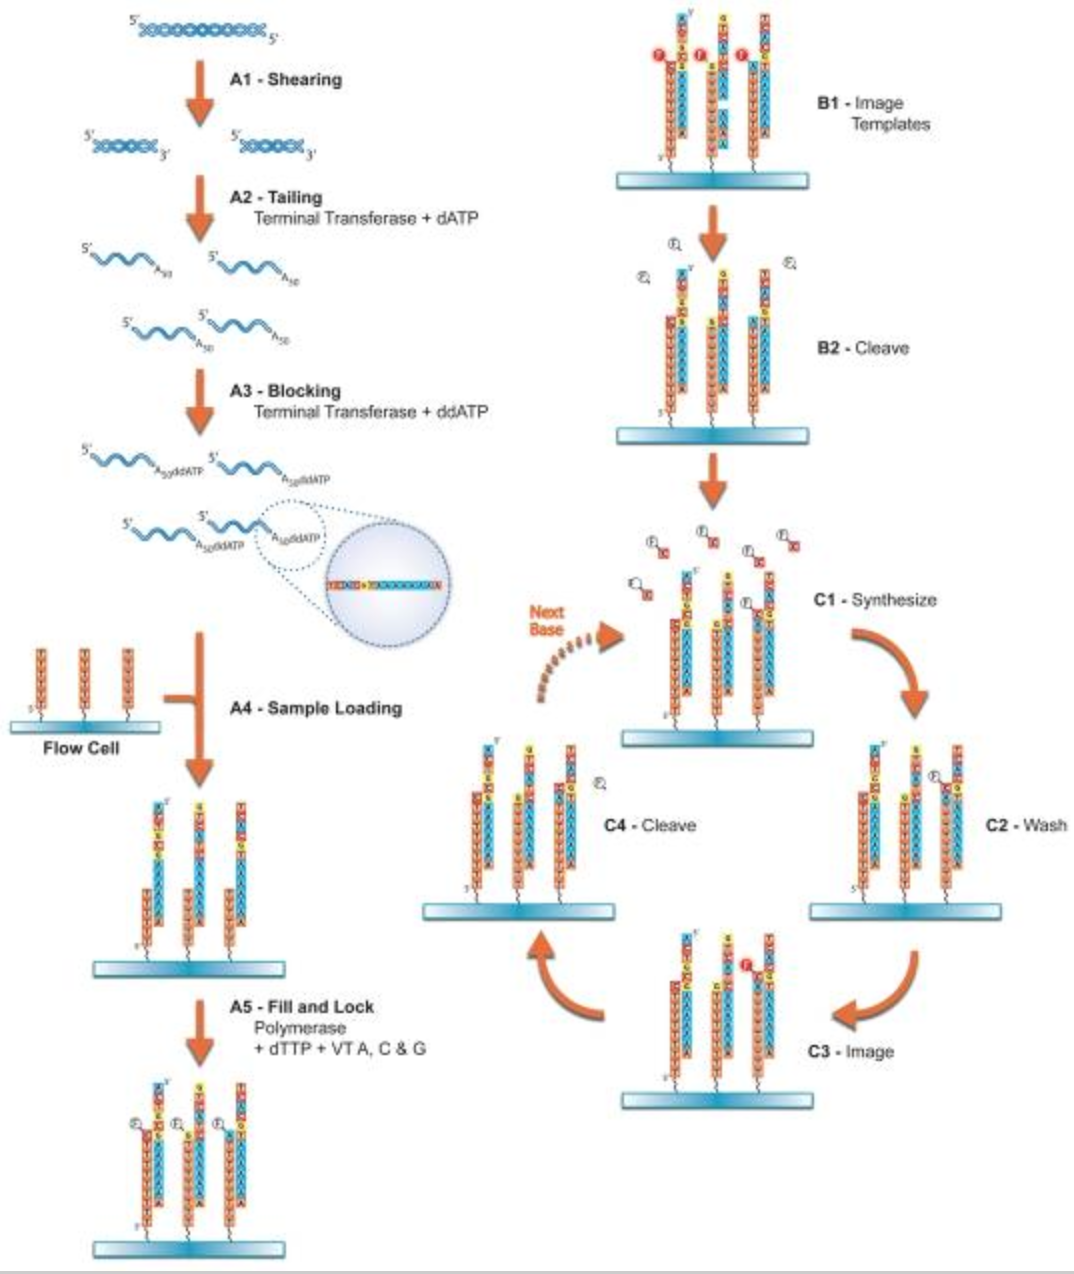
\includegraphics[width=0.5\textwidth]{c2.genomics/sequencing.sms.04.png}
  \end{figure}
\end{frame}

\begin{frame}
  \frametitle{基因组学 | 测序 | 第三代 | tSMS}
  \begin{block}{优缺点}
    真正的单分子测序,无需前期扩增,不引入偏向性;特别适合RNA-Seq或RNA直接测序的应用,因为它\textcolor{red}{能直接测序RNA模板},而无需将其转化成cDNA。检测碱基替换突变的误差率非常低,~0.2\%。\\
\vspace{1em}
缺点: 错误率高,Insertion 1.5\%,Deletion 3.0\%;Heliscope在面对同聚物时也会遇到一些困难,但可以通过二次测序提高准确度;由于在合成中可能掺有未标记的碱基,因此其最主要的错误来源是缺失。
  \end{block}
\end{frame}

\begin{frame}
  \frametitle{基因组学 | 测序 | 第三代 | SMRT}
  \begin{block}{概述}
PacBio SMRT(single molecule real time sequencing)技术也应用了边合成边测序的思想,并以SMRT芯片为测序载体。\\
\vspace{1em}
基本原理是:DNA聚合酶和模板结合,4色荧光标记4种碱基(即是dNTP),在碱基配对阶段,不同碱基的加入,会发出不同光,根据光的波长与峰值可判断进入的碱基类型。\\
\vspace{1em}
DNA聚合酶是实现超长读长的关键之一,读长主要跟酶的活性保持有关,它主要受激光对其造成的损伤所影响。
  \end{block}
\end{frame}

\begin{frame}
  \frametitle{基因组学 | 测序 | 第三代 | SMRT}
  \begin{block}{概述}
    PacBio SMRT技术的一个关键是怎样将反应信号与周围游离碱基的强大荧光背景区别出来。它们利用的是ZMW(Zero Mode Waveguide,零模波导孔)原理,如同微波炉壁上可看到的很多密集小孔。小孔直径有考究,如果直径大于微波波长,能量就会在衍射效应的作用下穿透面板而泄露出来,从而与周围小孔相互干扰。如果孔径小于波长,能量不会辐射到周围,而是保持直线状态(光衍射的原理),从而可起保护作用。同理,在一个反应管(SMRT Cell,单分子实时反应孔)中有许多这样的圆形纳米小孔,即ZMW(零模波导孔),外径100多纳米,比检测激光波长小(数百纳米),激光从底部打上去后不能穿透小孔进入上方溶液区,能量被限制在一个小范围(体积$20 \times 10^{-21}L$ )里,正好足够覆盖需要检测的部分,使得信号仅来自这个小反应区域,孔外过多游离核苷酸单体依然留在黑暗中,从而实现将背景降到最低。
  \end{block}
\end{frame}

\begin{frame}
  \frametitle{基因组学 | 测序 | 第三代 | SMRT}
  \begin{figure}
    \centering
    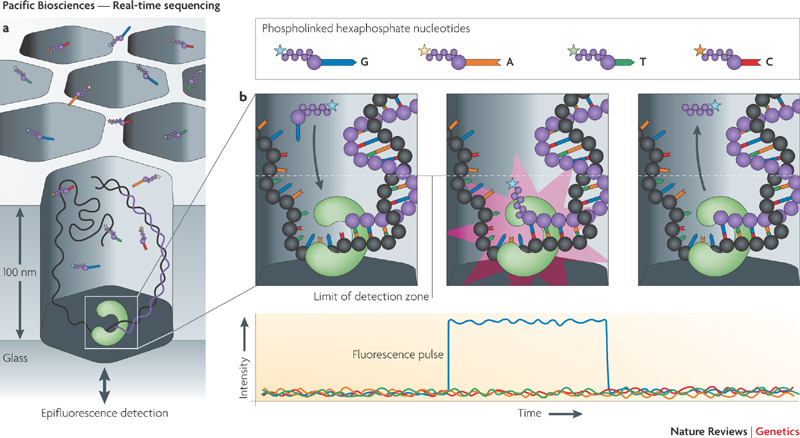
\includegraphics[width=0.9\textwidth]{c2.genomics/sequencing.smrt.01.jpg}
  \end{figure}
\end{frame}

\begin{frame}
  \frametitle{基因组学 | 测序 | 第三代 | SMRT}
  \begin{block}{优缺点}
可以通过检测相邻两个碱基之间的测序时间,来检测一些碱基修饰情况,即如果碱基存在修饰,则通过聚合酶时的速度会减慢,相邻两峰之间的距离增大,可以通过这个来\textcolor{red}{直接检测甲基化}等信息。\\
\vspace{1em}
SMRT技术的测序速度很快,每秒约10个dNTP。读长长。无需PCR扩增,也避免了由此带来的bias。需要的样品量很少,样品制备时间花费少。通量灵活,时间快。可以远程快速获取数据和选择测序参数。\\
\vspace{1em}
SMRT技术的测序错误率比较高(这几乎是目前单分子测序技术的通病),达到15\%,但好在它的出错是随机的,并不会像第二代测序技术那样存在测序错误的偏向,因而可以通过多次测序来进行有效的纠错。
  \end{block}
\end{frame}

\begin{frame}
  \frametitle{基因组学 | 测序 | 第三代 | SMRT}
  \begin{figure}
    \centering
    \includegraphics[width=0.9\textwidth]{c2.genomics/sequencing.smrt.03.jpg}
  \end{figure}
\end{frame}

\begin{frame}
  \frametitle{基因组学 | 测序 | 第三代 | FRET}
  \begin{block}{概述}
VisiGen基于荧光共振能量转移(FRET,Fluorescence Resonance Energy Transfer)的DNA测序技术。将标记了荧光供体基团的DNA聚合酶分子固定在载玻片上;再加含模板、引物、四种dNTP(其磷酸上标记特异的荧光受体基团)的测序缓冲液。\\
\vspace{1em}
测序延伸反应开始,带荧光受体基团的dNTP靠近含荧光供体基团的聚合酶,使后者释放能量,激发前者发出特异的荧光(即FRET信号),从而识别相应的碱基序列。当dNTP被加上后,荧光基团随磷酸离开,保证下一个dNTP能继续被加上。
  \end{block}
\end{frame}

\begin{frame}
  \frametitle{基因组学 | 测序 | 第三代 | FRET}
  \begin{figure}
    \centering
    \includegraphics[width=0.9\textwidth]{c2.genomics/sequencing.fret.01.jpg}
  \end{figure}
\end{frame}

\begin{frame}
  \frametitle{基因组学 | 测序 | 第三代 | 纳米孔测序}
  \begin{block}{概述}
Oxford Nanopore Technologies公司所开发的纳米单分子测序技术(Nanopore sequencing)与以往的测序技术皆不同,是基于电信号而不是光信号的测序技术。该技术的关键之一是,它们设计了一种特殊的纳米孔,孔内共价结合有分子接头。当DNA碱基通过纳米孔时,它们使电荷发生变化,从而短暂地影响流过纳米孔的电流强度(每种碱基所影响的电流变化幅度是不同的),灵敏的电子设备检测到这些变化从而鉴定所通过的碱基。
  \end{block}
\end{frame}

\begin{frame}
  \frametitle{基因组学 | 测序 | 第三代 | 纳米孔测序}
  \begin{figure}
    \centering
    \includegraphics[width=0.6\textwidth]{c2.genomics/sequencing.nano.01.jpg}
  \end{figure}
\end{frame}

\begin{frame}
  \frametitle{基因组学 | 测序 | 第三代 | 纳米孔测序}
  \begin{block}{优缺点}
纳米孔测序的主要特点是:读长很长,大约在几十kb,甚至100kb;错误率目前介于1\%至4\%,且是随机错误,而不是聚集在读段的两端;数据可实时读取;通量很高(30x人类基因组有望在一天内完成);起始DNA在测序过程中不被破坏;样品制备简单又便宜。理论上,它也\textcolor{red}{能直接测序RNA}。\\
\vspace{1em}
纳米孔单分子测序还有另外一大特点,它\textcolor{red}{能够直接读取出甲基化的胞嘧啶},而不必像传统方法那样对基因组进行bisulfite处理。这对于在基因组水平直接研究表观遗传相关现象有极大的帮助。并且该方法的测序准确性可达99.8\%,而且一旦发现测序错误也能较容易地进行纠正。
  \end{block}
\end{frame}

\begin{frame}
  \frametitle{基因组学 | 测序 | 第三代 | 纳米孔测序}
  \begin{figure}
    \centering
    \includegraphics[width=\textwidth]{c2.genomics/sequencing.nano.02.jpg}
  \end{figure}
\end{frame}

\begin{frame}
  \frametitle{基因组学 | 测序 | 第三代 | TEM}
  \begin{block}{概述}
以单链线性DNA为模板,以三种重元素标记、一种不标记的脱氧核苷酸为原料,合成其互补链,经透射电镜(TEM,Transmission electron microscopy)检测,则可见重元素标记,其互补链则可由点的大小和强度被分辨出来。
  \end{block}
\end{frame}

\begin{frame}
  \frametitle{基因组学 | 测序 | 第三代 | TEM}
  \begin{figure}
    \centering
    \includegraphics[width=0.9\textwidth]{c2.genomics/sequencing.tem.01.png}
  \end{figure}
\end{frame}

\begin{frame}
  \frametitle{基因组学 | 测序 | 第三代 | SMRT, Nanopore}
  \begin{figure}
    \centering
    \includegraphics[width=0.9\textwidth]{c2.genomics/sequencing.smrt.nano.02.png}
  \end{figure}
\end{frame}

\begin{frame}
  \frametitle{基因组学 | 测序 | 第三代 | SMRT, Nanopore}
  \begin{figure}
    \centering
    \includegraphics[width=0.8\textwidth]{c2.genomics/sequencing.smrt.nano.03.png}
  \end{figure}
\end{frame}

\begin{frame}
  \frametitle{基因组学 | 测序 | 第三代 | FRET, SMRT, tSMS}
  \begin{figure}
    \centering
    \includegraphics[width=0.9\textwidth]{c2.genomics/sequencing.fret.smrt.sms.01.jpg}
  \end{figure}
\end{frame}

\begin{frame}
  \frametitle{基因组学 | 测序 | 第三代 | tSMS, SMRT, FRET}
  \begin{figure}
    \centering
    \includegraphics[width=0.55\textwidth]{c2.genomics/sequencing.sms.smrt.fret.01.jpg}
  \end{figure}
\end{frame}

\begin{frame}
  \frametitle{基因组学 | 测序 | 第三代 | SMRT, FRET, Nanopore, Ion}
  \begin{figure}
    \centering
    \includegraphics[width=\textwidth]{c2.genomics/sequencing.smrt.fret.nano.ion.01.png}
  \end{figure}
\end{frame}

\subsection{测序技术比较}
\begin{frame}
  \frametitle{基因组学 | 测序 | 比较 | 公司}
  \begin{figure}
    \centering
    \includegraphics[width=0.9\textwidth]{c2.genomics/sequencing.logo.01.jpg}
  \end{figure}
\end{frame}

\begin{frame}
  \frametitle{基因组学 | 测序 | 比较 | 三代}
  \begin{figure}
    \centering
    \includegraphics[width=0.9\textwidth]{c2.genomics/sequencing.compare.20.jpg}
  \end{figure}
\end{frame}

\begin{frame}
  \frametitle{基因组学 | 测序 | 比较 | 三代}
  \begin{figure}
    \centering
    \includegraphics[width=0.9\textwidth]{c2.genomics/sequencing.compare.21.jpg}
  \end{figure}
\end{frame}

\begin{frame}
  \frametitle{基因组学 | 测序 | 比较 | 三代}
  \begin{figure}
    \centering
    \includegraphics[width=0.85\textwidth]{c2.genomics/sequencing.compare.22.jpg}
  \end{figure}
\end{frame}

\begin{frame}
  \frametitle{基因组学 | 测序 | 比较 | 三代}
  \begin{figure}
    \centering
    \includegraphics[width=0.9\textwidth]{c2.genomics/sequencing.compare.23.jpg}
  \end{figure}
\end{frame}

\begin{frame}
  \frametitle{基因组学 | 测序 | 比较 | 三代}
  \begin{figure}
    \centering
    \includegraphics[width=\textwidth]{c2.genomics/sequencing.compare.06.png}
  \end{figure}
\end{frame}

% \begin{frame}
%   \frametitle{基因组学 | 测序 | 比较}
%   \begin{figure}
%     \centering
%     \includegraphics[width=\textwidth]{c2.genomics/sequencing.compare.01.png}
%   \end{figure}
% \end{frame}

\begin{frame}
  \frametitle{基因组学 | 测序 | 比较 | 三代}
  \begin{figure}
    \centering
    \includegraphics[width=0.85\textwidth]{c2.genomics/sequencing.compare.02.png}
  \end{figure}
\end{frame}

% \begin{frame}
%   \frametitle{基因组学 | 测序 | 比较}
%   \begin{figure}
%     \centering
%     \includegraphics[width=\textwidth]{c2.genomics/sequencing.compare.11.png}
%   \end{figure}
% \end{frame}

\begin{frame}
  \frametitle{基因组学 | 测序 | 比较 | 三代}
  \begin{figure}
    \centering
    \includegraphics[width=0.6\textwidth]{c2.genomics/sequencing.compare.04.png}
  \end{figure}
\end{frame}

\begin{frame}
  \frametitle{基因组学 | 测序 | 比较 | 三代}
  \begin{figure}
    \centering
    \includegraphics[width=0.75\textwidth]{c2.genomics/sequencing.compare.05.png}
  \end{figure}
\end{frame}

\begin{frame}
  \frametitle{基因组学 | 测序 | 比较 | 测序仪}
  \begin{figure}
    \centering
    \includegraphics[width=0.85\textwidth]{c2.genomics/sequencing.compare.03.jpg}
  \end{figure}
\end{frame}

\begin{frame}
  \frametitle{基因组学 | 测序 | 比较 | 测序仪}
  \begin{figure}
    \centering
    \includegraphics[width=\textwidth]{c2.genomics/sequencing.compare.07.png}
  \end{figure}
\end{frame}

% \begin{frame}
%   \frametitle{基因组学 | 测序 | 比较 | 测序仪}
%   \begin{figure}
%     \centering
%     \includegraphics[width=\textwidth]{c2.genomics/sequencing.compare.08.png}
%   \end{figure}
% \end{frame}

\begin{frame}
  \frametitle{基因组学 | 测序 | 比较 | 测序仪}
  \begin{figure}
    \centering
    \includegraphics[width=\textwidth]{c2.genomics/sequencing.compare.09.png}
  \end{figure}
\end{frame}


\section{数据库与数据格式}
\subsection{数据库}
\begin{frame}
  \frametitle{基因组学 | 测序 | 数据库 | SRA}
  \begin{block}{SRA}
NCBI在2007年底推出了SRA数据库,专门用于存储、显示、提取和分析高通量测序数据。\\
\vspace{1em}
SRA数据库,最初的命名为Short Read Archive,现已改为Sequence Read Archive。\\
\vspace{1em}
Sequence Read Archive (SRA) makes biological sequence data available to the research community to enhance reproducibility and allow for new discoveries by comparing data sets. The SRA stores raw sequencing data and alignment information from high-throughput sequencing platforms, including Roche 454 GS System®, Illumina Genome Analyzer®, Applied Biosystems SOLiD System®, Helicos Heliscope®, Complete Genomics®, and Pacific Biosciences SMRT®. 
  \end{block}
\end{frame}
    
\begin{frame}
  \frametitle{基因组学 | 测序 | 数据库 | SRA}
  \begin{figure}
    \centering
    \includegraphics[width=0.7\textwidth]{c2.genomics/db.sra.05.png}
  \end{figure}
\end{frame}

\begin{frame}
  \frametitle{基因组学 | 测序 | 数据库 | SRA}
  \begin{figure}
    \centering
    \includegraphics[width=\textwidth]{c2.genomics/db.sra.01.png}
  \end{figure}
\end{frame}
    
\begin{frame}
  \frametitle{基因组学 | 测序 | 数据库 | SRA}
  \begin{figure}
    \centering
    \includegraphics[width=0.6\textwidth]{c2.genomics/db.sra.02.png}
  \end{figure}
\end{frame}
    
\begin{frame}
  \frametitle{基因组学 | 测序 | 数据库 | SRA}
  \begin{figure}
    \centering
    \includegraphics[width=0.9\textwidth]{c2.genomics/db.sra.03.png}
  \end{figure}
\end{frame}
    
\begin{frame}
  \frametitle{基因组学 | 测序 | 数据库 | SRA}
  \begin{figure}
    \centering
    \includegraphics[width=0.9\textwidth]{c2.genomics/db.sra.04.png}
  \end{figure}
\end{frame}
    
\begin{frame}
  \frametitle{基因组学 | 测序 | 数据库 | GEO}
  \begin{block}{GEO}
NCBI的GEO(Gene Expression Omnibus)数据库是一个非常强大的高通量数据集合,它综合了大量的芯片数据和二代测序数据,供全球科研工作者免费使用。\\
\vspace{1em}
NCBI的GEO数据库用于存储高通量的芯片实验数据,在SRA未建立之前,GEO数据库也用于存储高通量测序数据。\\
\vspace{1em}
GEO is a public functional genomics data repository supporting MIAME-compliant data submissions. Array- and sequence-based data are accepted. Tools are provided to help users query and download experiments and curated gene expression profiles.
  \end{block}
\end{frame}
    
\begin{frame}
  \frametitle{基因组学 | 测序 | 数据库 | GEO}
  \begin{figure}
    \centering
    \includegraphics[width=\textwidth]{c2.genomics/db.geo.01.png}
  \end{figure}
\end{frame}
    
\begin{frame}
  \frametitle{基因组学 | 测序 | 数据库 | GEO}
  \begin{figure}
    \centering
    \includegraphics[width=0.6\textwidth]{c2.genomics/db.geo.02.png}
  \end{figure}
\end{frame}

\begin{frame}
  \frametitle{基因组学 | 测序 | 数据库 | GEO}
  \begin{figure}
    \centering
    \includegraphics[width=0.6\textwidth]{c2.genomics/db.geo.03.png}
  \end{figure}
\end{frame}
    
\begin{frame}
  \frametitle{基因组学 | 测序 | 数据库 | 千人基因组计划}
  \begin{block}{千人基因组计划}
千人基因组计划(1000 Genomes Project),旨在绘制迄今(截至2011年)最详尽、最有医学应用价值的人类基因多态性图谱,该图谱由中美英等国科研机构发起的“千人基因组计划”共同协作完成,标志着人类基因研究取得重大突破。这项计划于2008年启动,目前该项目拥有超过1700个样本,高达200TB数据量的DNA序列。2012年开始全部数据将免费对外开放。
  \end{block}
\end{frame}
    
\begin{frame}
  \frametitle{基因组学 | 测序 | 数据库 | 千人基因组计划}
  \begin{figure}
    \centering
    \includegraphics[width=0.9\textwidth]{c2.genomics/db.1kg.01.png}
  \end{figure}
\end{frame}
    
\begin{frame}
  \frametitle{基因组学 | 测序 | 数据库 | 千人基因组计划}
  \begin{figure}
    \centering
    \includegraphics[width=0.9\textwidth]{c2.genomics/db.1kg.02.png}
  \end{figure}
\end{frame}
    
\begin{frame}
  \frametitle{基因组学 | 测序 | 数据库 | 千人基因组计划}
  \begin{figure}
    \centering
    \includegraphics[width=0.9\textwidth]{c2.genomics/db.1kg.03.png}
  \end{figure}
\end{frame}
    
\begin{frame}
  \frametitle{基因组学 | 测序 | 数据库 | TCGA}
  \begin{block}{TCGA}
Cancer Genome Atlas(TCGA)和International Cancer Consortium(ICGC)是目前国际上最大的两个癌症基因信息检索数据库,共收集了43种癌症的超过13万个样本数据,此外还涉及到相关癌症基因的mRNA/microRNA表达谱、拷贝数变异、突变等大量的生物信息学数据。
  \end{block}
\end{frame}

\begin{frame}
  \frametitle{基因组学 | 测序 | 数据库 | TCGA}
  \begin{figure}
    \centering
    \includegraphics[width=0.9\textwidth]{c2.genomics/db.tcga.01.png}
  \end{figure}
\end{frame}
    
\begin{frame}
  \frametitle{基因组学 | 测序 | 数据库 | TCGA}
  \begin{figure}
    \centering
    \includegraphics[width=0.9\textwidth]{c2.genomics/db.tcga.02.png}
  \end{figure}
\end{frame}

\begin{frame}
  \frametitle{基因组学 | 测序 | 数据库 | ICGC}
  \begin{figure}
    \centering
    \includegraphics[width=0.8\textwidth]{c2.genomics/db.icgc.01.png}
  \end{figure}
\end{frame}
    
\begin{frame}
  \frametitle{基因组学 | 测序 | 数据库 | ICGC}
  \begin{figure}
    \centering
    \includegraphics[width=0.9\textwidth]{c2.genomics/db.icgc.02.png}
  \end{figure}
\end{frame}
    
\subsection{数据格式}
\begin{frame}
  \frametitle{基因组学 | 测序 | 数据格式 | 概览}
  \begin{figure}
    \centering
    \includegraphics[width=0.9\textwidth]{c2.genomics/workflow.ngs.01.png}
  \end{figure}
\end{frame}
    
\begin{frame}
  \frametitle{基因组学 | 测序 | 数据格式 | 概览}
  \begin{figure}
    \centering
    \includegraphics[width=0.9\textwidth]{c2.genomics/workflow.ngs.02.png}
  \end{figure}
\end{frame}
    
\begin{frame}
  \frametitle{基因组学 | 测序 | 数据格式 | 概览}
  \begin{figure}
    \centering
    \includegraphics[width=0.9\textwidth]{c2.genomics/workflow.ngs.03.png}
  \end{figure}
\end{frame}
    
\begin{frame}
  \frametitle{基因组学 | 测序 | 数据格式 | 概览}
  \begin{figure}
    \centering
    \includegraphics[width=0.9\textwidth]{c2.genomics/workflow.ngs.04.png}
  \end{figure}
\end{frame}

\begin{frame}
  \frametitle{基因组学 | 测序 | 数据格式 | 概览}
  \begin{figure}
    \centering
    \includegraphics[width=0.9\textwidth]{c2.genomics/workflow.ngs.05.png}
  \end{figure}
\end{frame}

\begin{frame}
  \frametitle{基因组学 | 测序 | 数据格式 | 简介}
  \begin{figure}
    \centering
    \includegraphics[width=0.9\textwidth]{c2.genomics/format.list.01.jpg}
  \end{figure}
\end{frame}
    
\begin{frame}
  \frametitle{基因组学 | 测序 | 数据格式 | 简介}
  \begin{figure}
    \centering
    \includegraphics[width=0.9\textwidth]{c2.genomics/format.list.02.png}
  \end{figure}
\end{frame}

\begin{frame}
  \frametitle{基因组学 | 测序 | 数据格式 | 简介}
  \begin{block}{Reference sequences}
    \begin{itemize}
      \item FASTA
      \item 2bit
    \end{itemize}
  \end{block}
  \pause
  \begin{block}{Reads}
    \begin{itemize}
      \item FASTQ (FASTA with quality scores)
    \end{itemize}
  \end{block}
  \pause
  \begin{block}{Alignments}
    \begin{itemize}
      \item SAM (Sequence Alignment/Map format)
      \item BAM (Binary version of SAM)
    \end{itemize}
  \end{block}
\end{frame}
    
\begin{frame}
  \frametitle{基因组学 | 测序 | 数据格式 | 简介}
  \begin{block}{Features, annotation, coverage, scores}
    \begin{itemize}
      \item GFF3/GTF (General Feature Format, Gene Transfer Format)
      \item BED/bigBed (Browser Extensible Data)
      \item WIG/bigWig (Wiggle format)
      \item bedGraph
    \end{itemize}
  \end{block}
  \pause
  \begin{block}{Variations}
    \begin{itemize}
      \item VCF (Variant Call Format)
      \item BCF (Binary version of VCF)
    \end{itemize}
  \end{block}
\end{frame}
    
\begin{frame}
  \frametitle{基因组学 | 测序 | 数据格式 | FASTA}
  \begin{figure}
    \centering
    \includegraphics[width=0.9\textwidth]{c2.genomics/format.fasta.05.png}\\
    \vspace{1em}
    \includegraphics[width=0.9\textwidth]{c2.genomics/format.fasta.01.jpg}
  \end{figure}
\end{frame}
    
\begin{frame}
  \frametitle{基因组学 | 测序 | 数据格式 | FASTQ}
  \begin{block}{FASTQ}
FASTQ format is a text-based format for storing both a biological sequence (usually nucleotide sequence) and its corresponding quality scores. Both the sequence letter and quality score are each encoded with a single ASCII character for brevity.\\
\vspace{1em}
It was originally developed at the Wellcome Trust Sanger Institute to bundle a FASTA sequence and its quality data, but has recently become the de facto standard for storing the output of high-throughput sequencing instruments such as the Illumina Genome Analyzer.\\
\vspace{1em}
There is no standard file extension for a FASTQ file, but .fq and .fastq, are commonly used.
  \end{block}
\end{frame}
    
\begin{frame}
  \frametitle{基因组学 | 测序 | 数据格式 | FASTQ vs. FASTA}
  \begin{figure}
    \centering
    \includegraphics[width=\textwidth]{c2.genomics/format.fasta.fastq.01.png}
  \end{figure}
\end{frame}

\begin{frame}
  \frametitle{基因组学 | 测序 | 数据格式 | FASTQ}
  \begin{figure}
    \centering
    \includegraphics[width=\textwidth]{c2.genomics/format.fastq.02.png}
  \end{figure}
\end{frame}
    
\begin{frame}
  \frametitle{基因组学 | 测序 | 数据格式 | FASTQ}
  \begin{figure}
    \centering
    \includegraphics[width=0.9\textwidth]{c2.genomics/format.fastq.01.png}
  \end{figure}
\end{frame}
    
\begin{frame}
  \frametitle{基因组学 | 测序 | 数据格式 | FASTQ | ID}
  \begin{figure}
    \centering
    \includegraphics[width=0.9\textwidth]{c2.genomics/format.fastq.id.01.png}
  \end{figure}
\end{frame}
    
\begin{frame}
  \frametitle{基因组学 | 测序 | 数据格式 | FASTQ | ID}
  \begin{figure}
    \centering
    \includegraphics[width=0.9\textwidth]{c2.genomics/format.fastq.id.02.png}
  \end{figure}
\end{frame}
    
\begin{frame}
  \frametitle{基因组学 | 测序 | 数据格式 | FASTQ | ID}
  \begin{figure}
    \centering
    \includegraphics[width=0.9\textwidth]{c2.genomics/format.fastq.id.03.png}
  \end{figure}
\end{frame}
    
\begin{frame}
  \frametitle{基因组学 | 测序 | 数据格式 | FASTQ | SRA}
  \begin{figure}
    \centering
    \includegraphics[width=0.9\textwidth]{c2.genomics/format.fastq.sra.02.png}
  \end{figure}
  \begin{block}{Note}
    \begin{itemize}
      \item ID = NCBI-assigned identifier + the original identifier from Solexa/Illumina + the read length
      \item fastq-dump: lost the paired-end information, concatenate sequence of the forward and reverse reads together into a non-sense
      \item NCBI have converted this FASTQ data from the original Solexa/Illumina encoding to the Sanger standard
    \end{itemize}
  \end{block}
\end{frame}
    
\begin{frame}
  \frametitle{基因组学 | 测序 | 数据格式 | FASTQ | Quality}
  \begin{block}{Phred quality score}
A quality value Q is an integer mapping of p (i.e., the probability that the corresponding base call is incorrect).\\
\vspace{1em}
Phred quality score (the standard Sanger variant, assess reliability of a base call): 
  \end{block}
  \begin{figure}
    \centering
    \includegraphics[width=0.5\textwidth]{c2.genomics/format.fastq.qual.01.png}\\
    \vspace{1em}
    \includegraphics[width=0.8\textwidth]{c2.genomics/format.fastq.qual.02.png}
  \end{figure}
\end{frame}
    
\begin{frame}
  \frametitle{基因组学 | 测序 | 数据格式 | FASTQ | Quality | Encoding}
  \begin{figure}
    \centering
    \includegraphics[width=\textwidth]{c2.genomics/format.fastq.qual.04.png}
  \end{figure}
\end{frame}
    
\begin{frame}
  \frametitle{基因组学 | 测序 | 数据格式 | FASTQ | 用途}
  \begin{block}{Quality control}
    \begin{itemize}
      \item quality score distribution
      \item GC content
      \item k-mer enrichment
      \item ...
    \end{itemize}
  \end{block}
  \pause
  \begin{block}{Preprocessing}
    \begin{itemize}
      \item adapter removal
      \item low-quality reads filtering
      \item ...
    \end{itemize}
  \end{block}
  \pause
  \begin{block}{Processing}
    \begin{itemize}
      \item alignment
      \item further analysis
    \end{itemize}
  \end{block}
\end{frame}

\begin{frame}
  \frametitle{基因组学 | 测序 | 数据格式 | SAM}
  \begin{figure}
    \centering
    \includegraphics[width=\textwidth]{c2.genomics/format.sam.01.png}
  \end{figure}
  \begin{block}{SAM Format Specification}
    \href{https://samtools.github.io/hts-specs/SAMv1.pdf}{https://samtools.github.io/hts-specs/SAMv1.pdf}
  \end{block}
\end{frame}

\begin{frame}
  \frametitle{基因组学 | 测序 | 数据格式 | SAM}
  \begin{figure}
    \centering
    \includegraphics[width=0.9\textwidth]{c2.genomics/format.sam.02.png}\\
    \vspace{1em}
    \includegraphics[width=0.9\textwidth]{c2.genomics/format.sam.10.png}
  \end{figure}
\end{frame}

\begin{frame}
  \frametitle{基因组学 | 测序 | 数据格式 | SAM | FLAG}
  \begin{figure}
    \centering
    \includegraphics[width=0.9\textwidth]{c2.genomics/format.sam.flag.01.png}
  \end{figure}
  \begin{block}{Example}
    99 = 64 + 32 + 2 + 1
  \end{block}
  \begin{block}{Decoding SAM flags}
  \href{http://broadinstitute.github.io/picard/explain-flags.html}{http://broadinstitute.github.io/picard/explain-flags.html}
  \end{block}
\end{frame}

\begin{frame}
  \frametitle{基因组学 | 测序 | 数据格式 | SAM | FLAG}
  \begin{figure}
    \centering
    \includegraphics[width=0.8\textwidth]{c2.genomics/format.sam.flag.02.png}
  \end{figure}
\end{frame}

\begin{frame}
  \frametitle{基因组学 | 测序 | 数据格式 | SAM | CIGAR}
  \begin{figure}
    \centering
    \includegraphics[width=0.9\textwidth]{c2.genomics/format.sam.cigar.01.png}
  \end{figure}
\end{frame}

\begin{frame}
  \frametitle{基因组学 | 测序 | 数据格式 | SAM | CIGAR}
  \begin{figure}
    \centering
    \includegraphics[width=0.9\textwidth]{c2.genomics/format.sam.cigar.02.png}
  \end{figure}
\end{frame}

\begin{frame}
  \frametitle{基因组学 | 测序 | 数据格式 | SAM | TAG}
  \begin{figure}
    \centering
    \includegraphics[width=0.9\textwidth]{c2.genomics/format.sam.tag.01.png}
  \end{figure}
\end{frame}

\begin{frame}
  \frametitle{基因组学 | 测序 | 数据格式 | SAM}
  \begin{figure}
    \centering
    \includegraphics[width=0.6\textwidth]{c2.genomics/format.sam.03.png}\\
    \vspace{1em}
    \includegraphics[width=0.9\textwidth]{c2.genomics/format.sam.04.png}
  \end{figure}
\end{frame}
    
\begin{frame}
  \frametitle{基因组学 | 测序 | 数据格式 | BAM}
  \begin{figure}
    \centering
    \includegraphics[width=0.8\textwidth]{c2.genomics/format.bam.01.png}
  \end{figure}
\end{frame}
    
\begin{frame}
  \frametitle{基因组学 | 测序 | 数据格式 | BED}
  \begin{figure}
    \centering
    \includegraphics[width=0.9\textwidth]{c2.genomics/format.bed.01.jpg}
  \end{figure}
\end{frame}

\begin{frame}
  \frametitle{基因组学 | 测序 | 数据格式 | BED}
  \begin{figure}
    \centering
    \includegraphics[width=\textwidth]{c2.genomics/format.bed.10.png}
  \end{figure}
\end{frame}

\begin{frame}
  \frametitle{基因组学 | 测序 | 数据格式 | BED}
  \begin{block}{BED}
    \begin{itemize}
      \item Developed primarily for the UCSC genome browser
      \item Used to store annotations on genomic coordinates
        \begin{itemize}
          \item Annotate gene/mRNA/exon/... position
          \item Annotate Transcription Factor binding sites
          \item Annotate SNP genotypes
          \item Annotate Gene Expression
          \item Annotate ...
        \end{itemize}
    \end{itemize}
  \end{block}
\end{frame}
    
\begin{frame}
  \frametitle{基因组学 | 测序 | 数据格式 | GTF}
  \begin{figure}
    \centering
    \includegraphics[width=0.9\textwidth]{c2.genomics/format.gtf.01.jpg}
  \end{figure}
\end{frame}
    
\begin{frame}
  \frametitle{基因组学 | 测序 | 数据格式 | GTF}
  \begin{figure}
    \centering
    \includegraphics[width=\textwidth]{c2.genomics/format.gtf.10.png}
  \end{figure}
\end{frame}
    
\begin{frame}
  \frametitle{基因组学 | 测序 | 数据格式 | GFF}
  \begin{figure}
    \centering
    \includegraphics[width=0.9\textwidth]{c2.genomics/format.gff.01.jpg}
  \end{figure}
\end{frame}
    
\begin{frame}
  \frametitle{基因组学 | 测序 | 数据格式 | GFF}
  \begin{figure}
    \centering
    \includegraphics[width=\textwidth]{c2.genomics/format.gff.10.jpg}
  \end{figure}
\end{frame}
    
\begin{frame}
  \frametitle{基因组学 | 测序 | 数据格式 | GTF vs. GFF}
  \begin{figure}
    \centering
    \includegraphics[width=0.9\textwidth]{c2.genomics/format.gtf.gff.01.jpg}
  \end{figure}
\end{frame}

\begin{frame}
  \frametitle{基因组学 | 测序 | 数据格式 | BED vs. GFF}
  \begin{figure}
    \centering
    \includegraphics[width=0.9\textwidth]{c2.genomics/format.bed.gff.01.jpg}
  \end{figure}
\end{frame}
    
\begin{frame}
  \frametitle{基因组学 | 测序 | 数据格式 | BED vs. GFF}
  \begin{figure}
    \centering
    \includegraphics[width=\textwidth]{c2.genomics/format.bed.gff.02.jpg}
  \end{figure}
\end{frame}
    
\begin{frame}
  \frametitle{基因组学 | 测序 | 数据格式 | VCF}
  \begin{figure}
    \centering
    \includegraphics[width=0.9\textwidth]{c2.genomics/format.vcf.01.jpg}
  \end{figure}
\end{frame}
    
\begin{frame}
  \frametitle{基因组学 | 测序 | 数据格式 | VCF}
  \begin{figure}
    \centering
    \includegraphics[width=0.9\textwidth]{c2.genomics/format.vcf.02.jpg}
  \end{figure}
\end{frame}
    
\begin{frame}
  \frametitle{基因组学 | 测序 | 数据格式 | VCF}
  \begin{figure}
    \centering
    \includegraphics[width=0.9\textwidth]{c2.genomics/format.vcf.03.jpg}
  \end{figure}
\end{frame}

\begin{frame}
  \frametitle{基因组学 | 测序 | 数据格式 | VCF}
  \begin{figure}
    \centering
    \includegraphics[width=0.9\textwidth]{c2.genomics/format.vcf.04.jpg}
  \end{figure}
\end{frame}
    
\begin{frame}
  \frametitle{基因组学 | 测序 | 数据格式 | VCF}
  \begin{figure}
    \centering
    \includegraphics[width=\textwidth]{c2.genomics/format.vcf.05.png}
  \end{figure}
\end{frame}
    
\begin{frame}
  \frametitle{基因组学 | 测序 | 数据格式 | VCF}
  \begin{figure}
    \centering
    \includegraphics[width=\textwidth]{c2.genomics/format.vcf.13.png}
  \end{figure}
\end{frame}
    

\section{二代测序数据分析}
\subsection{常见术语}
\begin{frame}
  \frametitle{基因组学 | NGS | 数据分析 | 术语 | \textcolor{red}{深度 vs. 覆盖度}}
  \begin{block}{深度(depth)}
    \begin{itemize}
      \item 也叫乘数,衡量测序量的首要参数;测序得到的总碱基数与待测基因组大小的比值;每个碱基被测序的平均次数
      \item 假设一个基因大小为2M,测序获得的总数据量为20M,那么深度为10X
    \end{itemize}
  \end{block}
  \pause
  \begin{block}{覆盖度(coverage)}
    \begin{itemize}
      \item 测序获得的序列占整个基因组的比例
      \item 由于基因组中的高GC、重复序列等复杂结构的存在,测序最终拼接组装获得的序列往往无法覆盖所有的区域,这部分没有获得的区域就称为Gap。例如一个细菌基因组测序,覆盖度是98\%,那么还有2\%的序列区域是没有通过测序获得的。
    \end{itemize}
  \end{block}
\end{frame}

\begin{frame}
  \frametitle{基因组学 | NGS | 数据分析 | 术语 | 深度 vs. 覆盖度}
  \begin{block}{实验}
对长100bp的目标区域进行捕获测序:采用单端测序,每个read长5bp;总共得到了200个reads;把所有的reads比对到目标区域后,100bp的目标区域中有98bp的位置至少有1个read覆盖到,换言之,剩余的2bp没有1个read覆盖。
  \end{block}
  \pause
  \begin{block}{深度与覆盖度}
    \begin{itemize}
      \item 深度:$200 \times 5 / 100 = 10$
      \item 覆盖度:$98 / 100 \times 100\% = 98\%$
    \end{itemize}
  \end{block}
\end{frame}

\begin{frame}
  \frametitle{基因组学 | NGS | 数据分析 | 术语 | 深度 vs. 覆盖度}
  \begin{figure}
    \centering
    \includegraphics[width=0.85\textwidth]{c2.genomics/term.depth.cov.01.png}
  \end{figure}
\end{frame}

\begin{frame}
  \frametitle{基因组学 | NGS | 数据分析 | 术语 | SE vs. PE}
  \begin{figure}
    \centering
    \includegraphics[width=0.85\textwidth]{c2.genomics/term.se.pe.01.jpg}
  \end{figure}
\end{frame}

\begin{frame}
  \frametitle{基因组学 | NGS | 数据分析 | 术语 | SE vs. PE}
  \begin{figure}
    \centering
    \includegraphics[width=0.8\textwidth]{c2.genomics/term.se.pe.02.jpg}
  \end{figure}
\end{frame}

\begin{frame}
  \frametitle{基因组学 | NGS | 数据分析 | 术语 | PE}
  \begin{block}{Paired-End Sequencing}
    \begin{itemize}
      \item allows users to sequence both ends of a fragment and generate high-quality, alignable sequence data
      \item facilitates detection of genomic rearrangements and repetitive sequence elements, as well as gene fusions and novel transcripts
    \end{itemize}
  \end{block}
  \begin{figure}
    \centering
    \includegraphics[width=0.9\textwidth]{c2.genomics/term.pe.01.png}
  \end{figure}
\end{frame}

\begin{frame}
  \frametitle{基因组学 | NGS | 数据分析 | 术语 | PE}
  \begin{block}{Paired-End DNA Sequencing}
    \begin{itemize}
      \item provide superior alignment across DNA regions containing repetitive sequences
      \item produce longer contigs for \textit{de novo} sequencing by filling gaps in the consensus sequence
      \item detect rearrangements such as insertions, deletions, and inversions
    \end{itemize}
  \end{block}
  \pause
  \begin{block}{Paired-End RNA Sequencing}
    \begin{itemize}
      \item enable discovery applications such as detecting gene fusions in cancer and characterizing novel splice isoforms.
    \end{itemize}
  \end{block}
\end{frame}

\begin{frame}
  \frametitle{基因组学 | NGS | 数据分析 | 术语 | PE}
  \begin{figure}
    \centering
    \includegraphics[width=0.9\textwidth]{c2.genomics/term.se.pe.03.jpg}
  \end{figure}
\end{frame}

\begin{frame}
  \frametitle{基因组学 | NGS | 数据分析 | 术语 | PE | Power}
  \begin{figure}
    \centering
    \includegraphics[width=0.85\textwidth]{c2.genomics/term.pe.03.png}\\
    \vspace{1em}
    \includegraphics[width=0.85\textwidth]{c2.genomics/term.se.pe.04.png}
  \end{figure}
\end{frame}

\begin{frame}
  \frametitle{基因组学 | NGS | 数据分析 | 术语 | \textcolor{red}{PE}}
  \begin{figure}
    \centering
    \only<1->{\includegraphics[width=\textwidth]{c2.genomics/term.insert.size.01.png}}\\
    \vspace{1em}
    \only<2->{\includegraphics[width=\textwidth]{c2.genomics/term.insert.size.02.png}}
  \end{figure}
  \only<3->{
  \begin{block}{Conclusion}
    Remember that ``\textcolor{red}{insert}" refers to the DNA fragment between the adaptors, and not the gap between R1 and R2. Instead we refer to that as the ``\textcolor{red}{inner mate distance}".
  \end{block}
  }
\end{frame}

\begin{frame}
  \frametitle{基因组学 | NGS | 数据分析 | 术语 | \textcolor{red}{PE}}
  \begin{figure}
    \centering
    \includegraphics[width=0.85\textwidth]{c2.genomics/term.pe.02.png}
  \end{figure}
\end{frame}

\begin{frame}
  \frametitle{基因组学 | NGS | 数据分析 | 术语 | \textcolor{red}{其他}}
  \begin{figure}
    \centering
    \includegraphics[width=\textwidth]{c2.genomics/term.other.01.png}
  \end{figure}
\end{frame}

\subsection{分析流程}
\begin{frame}
  \frametitle{基因组学 | NGS | 数据分析 | 流程 | 概述 | 总览}
  \begin{figure}
    \centering
    \includegraphics[width=\textwidth]{c2.genomics/workflow.ngs.05.png}
  \end{figure}
\end{frame}

\begin{frame}
  \frametitle{基因组学 | NGS | 数据分析 | 流程 | 概述 | 总览}
  \begin{figure}
    \centering
    \includegraphics[width=\textwidth]{c2.genomics/workflow.ngs.01.png}
  \end{figure}
\end{frame}

\begin{frame}
  \frametitle{基因组学 | NGS | 数据分析 | 流程 | 概述 | 总览}
  \begin{figure}
    \centering
    \includegraphics[width=\textwidth]{c2.genomics/workflow.ngs.02.png}
  \end{figure}
\end{frame}

\begin{frame}
  \frametitle{基因组学 | NGS | 数据分析 | 流程 | 概述 | 总览}
  \begin{figure}
    \centering
    \includegraphics[width=0.85\textwidth]{c2.genomics/workflow.ngs.10.png}
  \end{figure}
\end{frame}

\begin{frame}
  \frametitle{基因组学 | NGS | 数据分析 | 流程 | 概述 | \textcolor{red}{Seqs}}
  \begin{figure}
    \centering
    \includegraphics[width=0.9\textwidth]{c2.genomics/workflow.ngs.03.png}
  \end{figure}
\end{frame}

\begin{frame}
  \frametitle{基因组学 | NGS | 数据分析 | 流程 | 概述 | Seqs}
  \begin{figure}
    \centering
    \includegraphics[width=\textwidth]{c2.genomics/workflow.ngs.04.png}
  \end{figure}
\end{frame}

\begin{frame}
  \frametitle{基因组学 | NGS | 数据分析 | 流程 | 概述 | \textcolor{red}{WES}}
  \begin{figure}
    \centering
    \includegraphics[width=0.6\textwidth]{c2.genomics/workflow.exome.05.png}
  \end{figure}
\end{frame}

\begin{frame}
  \frametitle{基因组学 | NGS | 数据分析 | 流程 | 概述 | \textcolor{red}{WES}}
  \begin{figure}
    \centering
    \includegraphics[width=0.9\textwidth]{c2.genomics/workflow.exome.03.png}
  \end{figure}
\end{frame}

\begin{frame}
  \frametitle{基因组学 | NGS | 数据分析 | 流程 | 质控(QC)}
  \begin{figure}
    \centering
    \includegraphics[width=0.9\textwidth]{c2.genomics/qc.pre.01.png}
  \end{figure}
\end{frame}

\begin{frame}
  \frametitle{基因组学 | NGS | 数据分析 | 流程 | 质控}
  \begin{figure}
    \centering
    \includegraphics[width=0.9\textwidth]{c2.genomics/qc.pre.02.png}
  \end{figure}
\end{frame}

\begin{frame}
  \frametitle{基因组学 | NGS | 数据分析 | 流程 | 质控}
  \begin{figure}
    \centering
    \includegraphics[width=0.9\textwidth]{c2.genomics/qc.pre.04.png}
  \end{figure}
\end{frame}

\begin{frame}
  \frametitle{基因组学 | NGS | 数据分析 | 流程 | 质控}
  \begin{figure}
    \centering
    \includegraphics[width=0.9\textwidth]{c2.genomics/qc.report.01.png}
  \end{figure}
\end{frame}

\begin{frame}
  \frametitle{基因组学 | NGS | 数据分析 | 流程 | 质控 | 工具}
  \begin{figure}
    \centering
    \includegraphics[width=\textwidth]{c2.genomics/qc.tool.01.png}
  \end{figure}
\end{frame}

\begin{frame}
  \frametitle{基因组学 | NGS | 数据分析 | 流程 | 质控 | \textcolor{red}{工具}}
  \begin{block}{FastQC}
    A quality control tool for high throughput sequence data.
  \end{block}
  \pause
  \begin{block}{NGS QC Toolkit}
    A toolkit for the quality control (QC) of next generation sequencing (NGS) data.
  \end{block}
  \pause
  \begin{block}{Others}
    \begin{itemize}
      \item SolexaQA: calculates sequence quality statistics and creates visual representations of data quality for second-generation sequencing data.
      \item ...
    \end{itemize}
  \end{block}
\end{frame}

\begin{frame}
  \frametitle{基因组学 | NGS | 数据分析 | 流程 | 质控 | FastQC}
  \begin{figure}
    \centering
    \includegraphics[width=0.9\textwidth]{c2.genomics/qc.fastqc.00.png}
  \end{figure}
\end{frame}

\begin{frame}
  \frametitle{基因组学 | NGS | 数据分析 | 流程 | 质控 | FastQC}
  \begin{figure}
    \centering
    \includegraphics[width=0.9\textwidth]{c2.genomics/qc.fastqc.03.png}
  \end{figure}
\end{frame}

\begin{frame}
  \frametitle{基因组学 | NGS | 数据分析 | 流程 | 质控 | FastQC}
  \begin{figure}
    \centering
    \includegraphics[width=0.9\textwidth]{c2.genomics/qc.fastqc.01.png}
  \end{figure}
\end{frame}

\begin{frame}
  \frametitle{基因组学 | NGS | 数据分析 | 流程 | 质控 | FastQC}
  \begin{figure}
    \centering
    \includegraphics[width=0.9\textwidth]{c2.genomics/qc.fastqc.02.png}
  \end{figure}
\end{frame}

\begin{frame}
  \frametitle{基因组学 | NGS | 数据分析 | 流程 | 质控 | FastQC}
  \begin{figure}
    \centering
    \includegraphics[width=\textwidth]{c2.genomics/qc.fastqc.10.png}
  \end{figure}
\end{frame}

\begin{frame}
  \frametitle{基因组学 | NGS | 数据分析 | 流程 | 质控 | FastQC}
  \begin{figure}
    \centering
    \includegraphics[width=\textwidth]{c2.genomics/qc.fastqc.11.png}
  \end{figure}
\end{frame}

\begin{frame}
  \frametitle{基因组学 | NGS | 数据分析 | 流程 | 质控 | FastQC}
  \begin{figure}
    \centering
    \includegraphics[width=\textwidth]{c2.genomics/qc.fastqc.30.png}
  \end{figure}
\end{frame}

\begin{frame}
  \frametitle{基因组学 | NGS | 数据分析 | 流程 | 质控 | FastQC}
  \begin{figure}
    \centering
    \includegraphics[width=\textwidth]{c2.genomics/qc.fastqc.12.png}
  \end{figure}
\end{frame}

\begin{frame}
  \frametitle{基因组学 | NGS | 数据分析 | 流程 | 质控 | FastQC}
  \begin{figure}
    \centering
    \includegraphics[width=\textwidth]{c2.genomics/qc.fastqc.13.png}
  \end{figure}
\end{frame}

\begin{frame}
  \frametitle{基因组学 | NGS | 数据分析 | 流程 | 质控 | FastQC}
  \begin{figure}
    \centering
    \includegraphics[width=\textwidth]{c2.genomics/qc.fastqc.14.png}
  \end{figure}
\end{frame}

\begin{frame}
  \frametitle{基因组学 | NGS | 数据分析 | 流程 | 质控 | FastQC}
  \begin{figure}
    \centering
    \includegraphics[width=\textwidth]{c2.genomics/qc.fastqc.15.png}
  \end{figure}
\end{frame}

\begin{frame}
  \frametitle{基因组学 | NGS | 数据分析 | 流程 | 质控 | FastQC}
  \begin{figure}
    \centering
    \includegraphics[width=0.9\textwidth]{c2.genomics/qc.fastqc.31.png}
  \end{figure}
\end{frame}

\begin{frame}
  \frametitle{基因组学 | NGS | 数据分析 | 流程 | 质控 | FastQC}
  \begin{figure}
    \centering
    \includegraphics[width=0.9\textwidth]{c2.genomics/qc.fastqc.32.png}
  \end{figure}
\end{frame}

\begin{frame}
  \frametitle{基因组学 | NGS | 数据分析 | 流程 | 质控 | FastQC}
  \begin{figure}
    \centering
    \includegraphics[width=\textwidth]{c2.genomics/qc.fastqc.16.png}
  \end{figure}
\end{frame}

\begin{frame}
  \frametitle{基因组学 | NGS | 数据分析 | 流程 | 质控 | FastQC}
  \begin{figure}
    \centering
    \includegraphics[width=\textwidth]{c2.genomics/qc.fastqc.17.png}
  \end{figure}
\end{frame}

\begin{frame}
  \frametitle{基因组学 | NGS | 数据分析 | 流程 | 质控 | FastQC}
  \begin{figure}
    \centering
    \includegraphics[width=\textwidth]{c2.genomics/qc.fastqc.18.png}
  \end{figure}
\end{frame}

\begin{frame}
  \frametitle{基因组学 | NGS | 数据分析 | 流程 | 质控 | FastQC}
  \begin{figure}
    \centering
    \includegraphics[width=\textwidth]{c2.genomics/qc.fastqc.19.png}
  \end{figure}
\end{frame}

\begin{frame}
  \frametitle{基因组学 | NGS | 数据分析 | 流程 | 质控 | FastQC}
  \begin{figure}
    \centering
    \includegraphics[width=\textwidth]{c2.genomics/qc.fastqc.20.png}
  \end{figure}
\end{frame}

\begin{frame}
  \frametitle{基因组学 | NGS | 数据分析 | 流程 | 质控 | FastQC}
  \begin{figure}
    \centering
    \includegraphics[width=0.9\textwidth]{c2.genomics/qc.fastqc.33.png}
  \end{figure}
\end{frame}

\begin{frame}
  \frametitle{基因组学 | NGS | 数据分析 | 流程 | 质控 | FastQC}
  \begin{figure}
    \centering
    \includegraphics[width=0.7\textwidth]{c2.genomics/qc.fastqc.34.png}
  \end{figure}
\end{frame}

\begin{frame}
  \frametitle{基因组学 | NGS | 数据分析 | 流程 | 质控 | FastQC}
  \begin{figure}
    \centering
    \includegraphics[width=0.85\textwidth]{c2.genomics/qc.fastqc.21.png}
  \end{figure}
\end{frame}

\begin{frame}
  \frametitle{基因组学 | NGS | 数据分析 | 流程 | 质控 | FastQC}
  \begin{figure}
    \centering
    \includegraphics[width=0.7\textwidth]{c2.genomics/qc.fastqc.36.png}
  \end{figure}
\end{frame}

\begin{frame}
  \frametitle{基因组学 | NGS | 数据分析 | 流程 | 质控 | FastQC}
  \begin{figure}
    \centering
    \includegraphics[width=0.8\textwidth]{c2.genomics/qc.fastqc.35.png}
  \end{figure}
\end{frame}

\begin{frame}
  \frametitle{基因组学 | NGS | 数据分析 | 流程 | 质控 | FastQC}
  \begin{figure}
    \centering
    \includegraphics[width=0.9\textwidth]{c2.genomics/qc.fastqc.22.png}
  \end{figure}
\end{frame}

\begin{frame}
  \frametitle{基因组学 | NGS | 数据分析 | 流程 | 质控 | FastQC}
  \begin{figure}
    \centering
    \includegraphics[width=0.9\textwidth]{c2.genomics/qc.fastqc.37.png}
  \end{figure}
\end{frame}

\begin{frame}
  \frametitle{基因组学 | NGS | 数据分析 | 流程 | 质控 | FastQC}
  \begin{figure}
    \centering
    \includegraphics[width=\textwidth]{c2.genomics/qc.fastqc.23.png}
  \end{figure}
\end{frame}

\begin{frame}
  \frametitle{基因组学 | NGS | 数据分析 | 流程 | 质控 | FastQC}
  \begin{figure}
    \centering
    \includegraphics[width=0.8\textwidth]{c2.genomics/qc.fastqc.24.png}
  \end{figure}
\end{frame}

\begin{frame}
  \frametitle{基因组学 | NGS | 数据分析 | 流程 | 质控 | FastQC}
  \begin{figure}
    \centering
    \includegraphics[width=0.7\textwidth]{c2.genomics/qc.fastqc.25.png}
  \end{figure}
\end{frame}

\begin{frame}
  \frametitle{基因组学 | NGS | 数据分析 | 流程 | 质控 | FastQC}
  \begin{figure}
    \centering
    \includegraphics[width=\textwidth]{c2.genomics/qc.fastqc.26.png}
  \end{figure}
\end{frame}

\begin{frame}
  \frametitle{基因组学 | NGS | 数据分析 | 流程 | 质控 | NGS QC Toolkit}
  \begin{figure}
    \centering
    \includegraphics[width=0.78\textwidth]{c2.genomics/qc.ngs.01.png}
  \end{figure}
\end{frame}

\begin{frame}
  \frametitle{基因组学 | NGS | 数据分析 | 流程 | 质控 | NGS QC Toolkit}
  \begin{figure}
    \centering
    \includegraphics[width=0.75\textwidth]{c2.genomics/qc.ngs.02.png}
  \end{figure}
\end{frame}

\begin{frame}
  \frametitle{基因组学 | NGS | 数据分析 | 流程 | 质控 | NGS QC Toolkit}
  \begin{figure}
    \centering
    \includegraphics[width=\textwidth]{c2.genomics/qc.ngs.03.png}
  \end{figure}
\end{frame}

\begin{frame}
  \frametitle{基因组学 | NGS | 数据分析 | 流程 | 质控 | NGS QC Toolkit}
  \begin{figure}
    \centering
    \includegraphics[width=0.9\textwidth]{c2.genomics/qc.ngs.04.png}
  \end{figure}
\end{frame}

\begin{frame}
  \frametitle{基因组学 | NGS | 数据分析 | 流程 | 质控 | SolexaQA}
  \begin{figure}
    \centering
    \includegraphics[width=\textwidth]{c2.genomics/qc.qa.01.png}
  \end{figure}
\end{frame}

\begin{frame}
  \frametitle{基因组学 | NGS | 数据分析 | 流程 | 质控 | SolexaQA}
  \begin{figure}
    \centering
    \includegraphics[width=\textwidth]{c2.genomics/qc.qa.02.png}
  \end{figure}
\end{frame}

\begin{frame}
  \frametitle{基因组学 | NGS | 数据分析 | 流程 | 质控 | SolexaQA}
  \begin{figure}
    \centering
    \includegraphics[width=\textwidth]{c2.genomics/qc.qa.03.png}
  \end{figure}
\end{frame}

\begin{frame}
  \frametitle{基因组学 | NGS | 数据分析 | 流程 | 预处理}
  \begin{block}{目的}
 manipulating the sequences to produce better mapping results
  \end{block}
  \pause
  \begin{block}{内容}
    \begin{itemize}
      \item Collapser: Collapsing identical sequences into a single sequence
      \item Clipper: Removing sequencing adapters/linkers
      \item Splitter: Splitting barcode containning multiple samples
      \item Filter: Filters sequences based on quality
      \item Trimmer: Trims (cuts) sequences based on quality
      \item Formatter: Rename identifiers, Reverse-complement, Mask nucleotides, Convert RNA $\leftrightarrow$ DNA, ...
      \item ...
    \end{itemize}
  \end{block}
\end{frame}

\begin{frame}
  \frametitle{基因组学 | NGS | 数据分析 | 流程 | 预处理}
  \begin{figure}
    \centering
    \includegraphics[width=0.7\textwidth]{c2.genomics/pre.01.jpg}
  \end{figure}
\end{frame}

\begin{frame}
  \frametitle{基因组学 | NGS | 数据分析 | 流程 | 预处理}
  \begin{figure}
    \centering
    \includegraphics[width=0.9\textwidth]{c2.genomics/pre.02.png}
  \end{figure}
\end{frame}

\begin{frame}
  \frametitle{基因组学 | NGS | 数据分析 | 流程 | 预处理 | \textcolor{red}{工具}}
  \begin{block}{FASTX-Toolkit}
    A collection of command line tools for Short-Reads FASTA/FASTQ files preprocessing.
  \end{block}
  \pause
  \begin{block}{PRINSEQ}
    PReprocessing and INformation of SEQuence data. A publicly available tool that is able to filter, reformat and trim your sequences and to provide you summary statistics for your sequence data.
  \end{block}
  \pause
  \begin{block}{cutadapt}
    Cutadapt finds and removes adapter sequences, primers, poly-A tails and other types of unwanted sequence from your high-throughput sequencing reads. It can also modify and filter reads in various ways.
  \end{block}
\end{frame}

\begin{frame}
  \frametitle{基因组学 | NGS | 数据分析 | 流程 | 预处理 | FASTX-Toolkit}
  \begin{figure}
    \centering
    \includegraphics[width=0.58\textwidth]{c2.genomics/pre.fastx.cli.01.png}
    \includegraphics[width=0.4\textwidth]{c2.genomics/pre.fastx.galaxy.01.png}
  \end{figure}
\end{frame}

\begin{frame}
  \frametitle{基因组学 | NGS | 数据分析 | 流程 | 预处理 | FASTX-Toolkit}
  \begin{figure}
    \centering
    \includegraphics[width=0.7\textwidth]{c2.genomics/pre.fastx.clip.01.png}
  \end{figure}
\end{frame}

\begin{frame}
  \frametitle{基因组学 | NGS | 数据分析 | 流程 | 预处理 | PRINSEQ}
  \begin{figure}
    \centering
    \includegraphics[width=0.6\textwidth]{c2.genomics/pre.prinseq.01.png}
  \end{figure}
\end{frame}

\begin{frame}
  \frametitle{基因组学 | NGS | 数据分析 | 流程 | 质控与预处理}
  \begin{figure}
    \centering
    \includegraphics[width=0.9\textwidth]{c2.genomics/qc.pre.03.png}
  \end{figure}
\end{frame}

\begin{frame}
  \frametitle{基因组学 | NGS | 数据分析 | 流程 | 比对}
  \begin{figure}
    \centering
    \includegraphics[width=0.9\textwidth]{c2.genomics/mapping.01.png}
  \end{figure}
\end{frame}

\begin{frame}
  \frametitle{基因组学 | NGS | 数据分析 | 流程 | 比对}
  \begin{figure}
    \centering
    \includegraphics[width=0.9\textwidth]{c2.genomics/mapping.07.png}
  \end{figure}
\end{frame}

\begin{frame}
  \frametitle{基因组学 | NGS | 数据分析 | 流程 | 比对}
  \begin{figure}
    \centering
    \includegraphics[width=0.9\textwidth]{c2.genomics/mapping.10.png}
  \end{figure}
\end{frame}

\begin{frame}
  \frametitle{基因组学 | NGS | 数据分析 | 流程 | 比对}
  \begin{figure}
    \centering
    \includegraphics[width=0.9\textwidth]{c2.genomics/mapping.08.png}
  \end{figure}
\end{frame}

\begin{frame}
  \frametitle{基因组学 | NGS | 数据分析 | 流程 | 比对 | 算法}
  \begin{figure}
    \centering
    \includegraphics[width=0.9\textwidth]{c2.genomics/mapping.02.png}
  \end{figure}
\end{frame}

\begin{frame}
  \frametitle{基因组学 | NGS | 数据分析 | 流程 | 比对 | 算法}
  \begin{figure}
    \centering
    \includegraphics[width=0.9\textwidth]{c2.genomics/mapping.09.png}
  \end{figure}
\end{frame}

\begin{frame}
  \frametitle{基因组学 | NGS | 数据分析 | 流程 | 比对 | 算法}
  \begin{figure}
    \centering
    \includegraphics[width=0.9\textwidth]{c2.genomics/mapping.03.jpg}
  \end{figure}
\end{frame}

\begin{frame}
  \frametitle{基因组学 | NGS | 数据分析 | 流程 | 比对 | 算法}
  \begin{figure}
    \centering
    \includegraphics[width=0.9\textwidth]{c2.genomics/mapping.05.jpg}
  \end{figure}
\end{frame}

\begin{frame}
  \frametitle{基因组学 | NGS | 数据分析 | 流程 | 比对 | 算法 | BWT}
  \begin{figure}
    \centering
    \includegraphics[width=0.9\textwidth]{c2.genomics/mapping.06.jpg}
  \end{figure}
\end{frame}

\begin{frame}
  \frametitle{基因组学 | NGS | 数据分析 | 流程 | 比对 | 算法 | BWT}
  \begin{figure}
    \centering
    \includegraphics[width=0.9\textwidth]{c2.genomics/mapping.bwt.01.jpg}
  \end{figure}
\end{frame}

\begin{frame}
  \frametitle{基因组学 | NGS | 数据分析 | 流程 | 比对 | 算法 | BWT}
  \begin{figure}
    \centering
    \includegraphics[width=\textwidth]{c2.genomics/mapping.bwt.02.jpg}
  \end{figure}
\end{frame}

\begin{frame}
  \frametitle{基因组学 | NGS | 数据分析 | 流程 | 比对 | 算法}
  \begin{figure}
    \centering
    \includegraphics[width=0.9\textwidth]{c2.genomics/mapping.04.jpg}
  \end{figure}
\end{frame}

\begin{frame}
  \frametitle{基因组学 | NGS | 数据分析 | 流程 | 比对 | 算法}
  \begin{figure}
    \centering
    \includegraphics[width=0.65\textwidth]{c2.genomics/mapping.11.png}
  \end{figure}
\end{frame}

\begin{frame}
  \frametitle{基因组学 | NGS | 数据分析 | 流程 | 比对 | 工具}
  \begin{figure}
    \centering
    \includegraphics[width=0.9\textwidth]{c2.genomics/tool.alignment.02.png}
  \end{figure}
\end{frame}

\begin{frame}
  \frametitle{基因组学 | NGS | 数据分析 | 流程 | 比对 | 工具}
  \begin{figure}
    \centering
    \includegraphics[width=0.9\textwidth]{c2.genomics/tool.alignment.03.png}
  \end{figure}
\end{frame}

\begin{frame}
  \frametitle{基因组学 | NGS | 数据分析 | 流程 | 比对 | 工具}
  \begin{figure}
    \centering
    \includegraphics[width=0.8\textwidth]{c2.genomics/tool.alignment.04.png}
  \end{figure}
\end{frame}

\begin{frame}
  \frametitle{基因组学 | NGS | 数据分析 | 流程 | 比对 | 工具}
  \begin{figure}
    \centering
    \includegraphics[width=0.9\textwidth]{c2.genomics/tool.alignment.01.png}
  \end{figure}
\end{frame}

\begin{frame}
  \frametitle{基因组学 | NGS | 数据分析 | 流程 | 比对 | \textcolor{red}{工具}}
  \begin{block}{BWA}
    BWA(Burrows-Wheeler Aligner) is a software package for mapping low-divergent sequences against a large reference genome, such as the human genome.
  \end{block}
  \pause
  \begin{block}{Bowtie}
    \begin{itemize}
      \item Bowtie is an ultrafast, memory-efficient short read aligner.
      \item Bowtie 2 is an ultrafast and memory-efficient tool for aligning sequencing reads to long reference sequences.
    \end{itemize}
  \end{block}
\end{frame}


\begin{frame}
  \frametitle{基因组学 | NGS | 数据分析 | 流程 | 比对 | \textcolor{red}{工具}}
  \begin{block}{SOAP}
    SOAP has been in evolution from a single alignment tool to a tool package that provides full solution to next generation sequencing data analysis.
    \begin{itemize}
      \item SOAPaligner/soap2: new alignment tool
      \item SOAPsnp: re-sequencing consensus sequence builder
      \item SOAPindel: indel finder
      \item SOAPsv: structural variation scanner
      \item SOAPdenovo: \textit{de novo} shot reads assembler
      \item SOAP3/GPU: GPU-accelerated alignment tool
    \end{itemize}
  \end{block}
\end{frame}

\begin{frame}
  \frametitle{基因组学 | NGS | 数据分析 | 流程 | 比对 | BWA}
  \begin{block}{BWA}
     BWA consists of three algorithms: BWA-backtrack, BWA-SW and BWA-MEM.
    \begin{itemize}
      \item BWA-backtrack is designed for Illumina sequence reads up to 100bp, while BWA-SW and BWA-MEM for longer sequences ranged from 70bp to 1Mbp.
      \item BWA-MEM and BWA-SW share similar features such as long-read support and split alignment.
      \item BWA-MEM, which is the latest, is generally recommended for high-quality queries as it is faster and more accurate. BWA-MEM also has better performance than BWA-backtrack for 70-100bp Illumina reads.
    \end{itemize}
  \end{block}
\end{frame}

\begin{frame}
  \frametitle{基因组学 | NGS | 数据分析 | 流程 | 比对 | Bowtie}
  \begin{block}{Bowtie}
 Bowtie aligns short DNA sequences (reads) to the human genome at a rate of over 25 million 35-bp reads per hour. Bowtie indexes the genome with a Burrows-Wheeler index to keep its memory footprint small: typically about 2.2 GB for the human genome (2.9 GB for paired-end).
  \end{block}
  \pause
  \begin{block}{Bowtie 2}
    Bowtie 2 is particularly good at aligning reads of about 50 up to 100s or 1,000s of characters, and particularly good at aligning to relatively long (e.g. mammalian) genomes. Bowtie 2 indexes the genome with an FM Index to keep its memory footprint small: for the human genome, its memory footprint is typically around 3.2 GB. Bowtie 2 supports gapped, local, and paired-end alignment modes.
  \end{block}
\end{frame}

\begin{frame}
  \frametitle{基因组学 | NGS | 数据分析 | 流程 | 比对 | SOAP}
  \begin{block}{SOAP}
    SOAP is a program for efficient gapped and ungapped alignment of short oligonucleotides onto reference sequences.
  \end{block}
  \pause
  \begin{block}{SOAP2}
    SOAPaligner/soap2 is an updated version of SOAP software for short oligonucleotide alignment. The new program features in super fast and accurate alignment for huge amounts of short reads generated by Illumina/Solexa Genome Analyzer.
  \end{block}
  \pause
  \begin{block}{SOAP3}
    SOAP3 is a GPU-based software for aligning short reads with a reference sequence. It can find all alignments with k mismatches, where k is chosen from 0 to 3. When compared with its previous version SOAP2, SOAP3 can be up to tens of times faster.
  \end{block}
\end{frame}

\begin{frame}
  \frametitle{基因组学 | NGS | 数据分析 | 流程 | 提取变异}
  \begin{figure}
    \centering
    \includegraphics[width=0.9\textwidth]{c2.genomics/snp.calling.01.jpg}
  \end{figure}
\end{frame}

\begin{frame}
  \frametitle{基因组学 | NGS | 数据分析 | 流程 | 提取变异 | \textcolor{red}{工具}}
  \begin{block}{SAMtools}
    SAMtools is a suite of programs for interacting with high-throughput sequencing data.
  \end{block}
  \pause
  \begin{block}{GATK}
    Genome Analysis Toolkit: Variant Discovery in High-Throughput Sequencing Data.\\
    The GATK toolkit offers a wide variety of tools with a primary focus on variant discovery and genotyping.
  \end{block}
  \pause
  \begin{block}{VarScan}
    VarScan is a platform-independent software tool developed at the Genome Institute at Washington University to detect variants in NGS data.
  \end{block}
\end{frame}

\begin{frame}
  \frametitle{基因组学 | NGS | 数据分析 | 流程 | 提取变异 | SAMtools}
  \begin{block}{SAMtools}
    SAMtools consists of three separate repositories:
    \begin{description}
      \item[SAMtools] Reading/writing/editing/indexing/viewing SAM/BAM/CRAM format
      \item[BCFtools] Reading/writing BCF2/VCF/gVCF files and calling/filtering/summarising SNP and short indel sequence variants
      \item[HTSlib] A C library for reading/writing high-throughput sequencing data
    \end{description}
  \end{block}
\end{frame}

\begin{frame}
  \frametitle{基因组学 | NGS | 数据分析 | 流程 | 提取变异 | GATK}
  \begin{figure}
    \centering
    \includegraphics[width=0.9\textwidth]{c2.genomics/snp.calling.gatk.01.png}\\
    \vspace{1em}
    \includegraphics[width=0.9\textwidth]{c2.genomics/snp.calling.gatk.02.png}
  \end{figure}
\end{frame}

\begin{frame}
  \frametitle{基因组学 | NGS | 数据分析 | 流程 | 提取变异 | VarScan}
  \begin{block}{VarScan}
    VarScan is a platform-independent mutation caller for targeted, exome, and whole-genome resequencing data generated on Illumina, SOLiD, Life/PGM, Roche/454, and similar instruments. It can be used to detect different types of variation:
    \begin{itemize}
      \item Germline variants (SNPs and indels) in individual samples or pools of samples.
      \item Multi-sample variants (shared or private) in multi-sample datasets (with mpileup).
      \item Somatic mutations, LOH events, and germline variants in tumor-normal pairs.
      \item Somatic copy number alterations (CNAs) in tumor-normal exome data.
    \end{itemize}
  \end{block}
\end{frame}

\begin{frame}
  \frametitle{基因组学 | NGS | 数据分析 | 流程 | 注释变异 | \textcolor{red}{工具}}
  \begin{block}{SnpEff}
    Genetic variant annotation and effect prediction toolbox. It annotates and predicts the effects of variants on genes (such as amino acid changes).
  \end{block}
  \pause
  \begin{block}{ANNOVAR}
    ANNOVAR is an efficient software tool to utilize update-to-date information to functionally annotate genetic variants detected from diverse genomes (including human genome hg18, hg19, hg38, as well as mouse, worm, fly, yeast and many others).
  \end{block}
  \pause
  \begin{block}{SeattleSeq Annotation}
    The SeattleSeq Annotation server provides annotation of SNVs (single-nucleotide variations) and small indels, both known and novel.
  \end{block}
\end{frame}

\begin{frame}
  \frametitle{基因组学 | NGS | 数据分析 | 流程 | 注释变异 | SnpEff}
  \begin{block}{Features}
    \begin{itemize}
      \item Supports over 38,000 genomes
      \item Standard ANN annotation format
      \item Cancer variants analysis
      \item GATK compatible (-o gatk)
      \item HGVS notation
      \item Sequence Ontology standardized terms
    \end{itemize}
  \end{block}
\end{frame}

\begin{frame}
  \frametitle{基因组学 | NGS | 数据分析 | 流程 | 注释变异 | ANNOVAR}
  \begin{block}{ANNOVAR}
    Given a list of variants with chromosome, start position, end position, reference nucleotide and observed nucleotides, ANNOVAR can perform:
    {\footnotesize
      \begin{description}
      \item[Gene-based annotation] identify whether SNPs or CNVs cause protein coding changes and the amino acids that are affected.
      \item[Region-based annotation] identify variants in specific genomic regions (conserved regions among 44 species, database of genomic variants, or many other annotations on genomic intervals).
      \item[Filter-based annotation] identify variants that are documented in specific databases, (whether a variant is reported in dbSNP, calculate the SIFT/PolyPhen/... scores, or many other annotations on specific mutations).
      \item[Other functionalities] Retrieve the nucleotide sequence in any user-specific genomic positions in batch, identify a candidate gene list for Mendelian diseases from exome data, and other utilities.
    \end{description}
    }
  \end{block}
\end{frame}

\begin{frame}
  \frametitle{基因组学 | NGS | 数据分析 | 流程 | 注释变异 | wANNOVAR}
  \begin{block}{wANNOVAR}
  wANNOVAR is a web server that provides easy and intuitive web-based access to the most popular functionalities of the ANNOVAR software.\\
  \vspace{0.5em}
  Users can upload a VCF file and obtain annotated results as tab-delimited or comma-deleted files; in addition, simple variants reduction can be performed to prioritize deleterious variants from the input files.\\
  \vspace{0.5em}
  Currently, wANNOVAR supports only human genome annotation.
  \end{block}
\end{frame}

\begin{frame}
  \frametitle{基因组学 | NGS | 数据分析 | 流程 | 注释变异 | SeattleSeq}
  \begin{block}{SeattleSeq Annotation}
  This annotation includes:
  \begin{itemize}
    \item dbSNP rs IDs
    \item gene names and accession numbers
    \item variation functions (e.g. missense)
    \item protein positions and amino-acid changes
    \item conservation scores
    \item HapMap frequencies
    \item PolyPhen predictions
    \item clinical association
  \end{itemize}
  \end{block}
\end{frame}

\begin{frame}
  \frametitle{基因组学 | NGS | 数据分析 | 流程 | 注释变异 | \textcolor{red}{工具}}
  \begin{block}{SIFT}
    SIFT predicts whether an amino acid substitution affects protein function. SIFT prediction is based on the degree of conservation of amino acid residues in sequence alignments derived from closely related sequences, collected through PSI-BLAST. SIFT can be applied to naturally occurring nonsynonymous polymorphisms or laboratory-induced missense mutations.
  \end{block}
  \pause
  \begin{block}{PolyPhen-2}
    PolyPhen-2 (Polymorphism Phenotyping v2) is a tool which predicts possible impact of an amino acid substitution on the structure and function of a human protein using straightforward physical and comparative considerations.
  \end{block}
\end{frame}

\begin{frame}
  \frametitle{基因组学 | NGS | 数据分析 | 流程 | 注释变异 | SIFT}
  \begin{figure}
    \centering
    \includegraphics[width=0.9\textwidth]{c2.genomics/snp.annotation.sift.01.png}
  \end{figure}
\end{frame}

\begin{frame}
  \frametitle{基因组学 | NGS | 数据分析 | 流程 | 注释变异 | PolyPhen-2}
  \begin{figure}
    \centering
    \includegraphics[width=0.7\textwidth]{c2.genomics/snp.annotation.polyphen2.01.png}
  \end{figure}
\end{frame}

\begin{frame}
  \frametitle{基因组学 | NGS | 数据分析 | 流程 | 可视化 | \textcolor{red}{工具}}
  \begin{block}{Genome Browser}
    interactively visualize genomic data
  \end{block}
  \pause
  \begin{block}{IGV}
    The Integrative Genomics Viewer (IGV) is a high-performance visualization tool for interactive exploration of large, integrated genomic datasets.
  \end{block}
  \pause
  \begin{block}{Tablet}
    Tablet is a lightweight, high-performance graphical viewer for next generation sequence assemblies and alignments.
  \end{block}
  \pause
  \begin{block}{Circos}
    Circos is a software package for visualizing data and information. It visualizes data in a circular layout --- this makes Circos ideal for exploring relationships between objects or positions.
  \end{block}
\end{frame}

\begin{frame}
  \frametitle{基因组学 | NGS | 数据分析 | 流程 | 可视化 | Genome Browser}
  \begin{figure}
    \centering
    \includegraphics[width=0.9\textwidth]{c2.genomics/vis.gb.01.jpg}
  \end{figure}
\end{frame}

\begin{frame}
  \frametitle{基因组学 | NGS | 数据分析 | 流程 | 可视化 | IGV}
  \begin{figure}
    \centering
    \includegraphics[width=0.9\textwidth]{c2.genomics/vis.igv.10.png}
  \end{figure}
\end{frame}

\begin{frame}
  \frametitle{基因组学 | NGS | 数据分析 | 流程 | 可视化 | IGV}
  \begin{figure}
    \centering
    \includegraphics[width=0.9\textwidth]{c2.genomics/vis.igv.11.png}
  \end{figure}
\end{frame}

\begin{frame}
  \frametitle{基因组学 | NGS | 数据分析 | 流程 | 可视化 | IGV}
  \begin{figure}
    \centering
    \includegraphics[width=0.85\textwidth]{c2.genomics/vis.igv.03.jpg}
  \end{figure}
\end{frame}

\begin{frame}
  \frametitle{基因组学 | NGS | 数据分析 | 流程 | 可视化 | IGV}
  \begin{figure}
    \centering
    \includegraphics[width=0.95\textwidth]{c2.genomics/vis.igv.02.png}
  \end{figure}
\end{frame}

\begin{frame}
  \frametitle{基因组学 | NGS | 数据分析 | 流程 | 可视化 | GB vs. IGV}
  \begin{figure}
    \centering
    \includegraphics[width=0.9\textwidth]{c2.genomics/vis.gb.igv.01.png}
  \end{figure}
\end{frame}

\begin{frame}
  \frametitle{基因组学 | NGS | 数据分析 | 流程 | 可视化 | Tablet}
  \begin{figure}
    \centering
    \includegraphics[width=0.85\textwidth]{c2.genomics/vis.tablet.01.png}
  \end{figure}
\end{frame}

\begin{frame}
  \frametitle{基因组学 | NGS | 数据分析 | 流程 | 可视化 | Circos}
  \begin{figure}
    \centering
    \includegraphics[width=0.5\textwidth]{c2.genomics/vis.circos.01.png}
  \end{figure}
\end{frame}

\begin{frame}
  \frametitle{基因组学 | NGS | 数据分析 | 流程 | 可视化 | Circos}
  \begin{figure}
    \centering
    \includegraphics[width=0.6\textwidth]{c2.genomics/vis.circos.03.png}
  \end{figure}
\end{frame}

\begin{frame}
  \frametitle{基因组学 | NGS | 数据分析 | 流程 | \textcolor{red}{补遗}}
  \begin{block}{bedtools}
    Collectively, the bedtools utilities are a swiss-army knife of tools for a wide-range of genomics analysis tasks. The most widely-used tools enable genome arithmetic: that is, set theory on the genome.
  \end{block}
  \pause
  \begin{block}{BEDOPS}
    BEDOPS is an open-source command-line toolkit that performs highly efficient and scalable Boolean and other set operations, statistical calculations, archiving, conversion and other management of genomic data of arbitrary scale.
  \end{block}
\end{frame}

\begin{frame}
  \frametitle{基因组学 | NGS | 数据分析 | 流程 | 补遗 | bedtools}
  \begin{figure}
    \centering
    \includegraphics[width=0.6\textwidth]{c2.genomics/tools.other.bedtools.01.png}
  \end{figure}
\end{frame}

\begin{frame}
  \frametitle{基因组学 | NGS | 数据分析 | 流程 | 补遗 | BEDOPS}
  \begin{figure}
    \centering
    \includegraphics[width=0.9\textwidth]{c2.genomics/tools.other.bedops.01.png}
  \end{figure}
\end{frame}

\begin{frame}
  \frametitle{基因组学 | NGS | 数据分析 | 流程 | \textcolor{red}{补遗}}
  \begin{block}{Picard}
    Picard is a set of command line tools for manipulating high-throughput sequencing (HTS) data and formats such as SAM/BAM/CRAM and VCF.
  \end{block}
  \pause
  \begin{block}{csvkit}
    csvkit is a suite of command-line tools for converting to and working with CSV, the king of tabular file formats.
  \end{block}
\end{frame}

\begin{frame}
  \frametitle{基因组学 | NGS | 数据分析 | 流程 | 补遗 | csvkit}
  \begin{block}{csvkit}
    \begin{description}
      \item[in2csv] the Excel killer
      \item[csvlook] data periscope
      \item[csvcut] data scalpel
      \item[csvstat] statistics without code
      \item[csvgrep] find the data you need
      \item[csvsort] order matters
      \item[csvjoin] merging related data
      \item[csvstack] combining subsets
      \item[csvsql \& sql2csv] ultimate power
      \item[csvjson] going online
      \item[csvpy] going into code
      \item[csvformat] for legacy systems
      \item[csvclean] clean common syntax errors
    \end{description}
  \end{block}
\end{frame}

\begin{frame}
  \frametitle{基因组学 | NGS | 数据分析 | 流程 | 补遗 | 工作流}
  \begin{figure}
    \centering
    \includegraphics[width=0.9\textwidth]{c2.genomics/tool.other.01.png}
  \end{figure}
\end{frame}

\begin{frame}
  \frametitle{基因组学 | NGS | 数据分析 | 流程 | 补遗 | \textcolor{red}{工作流}}
  {\small
  \begin{block}{Bpipe}
    Bpipe provides a platform for running big bioinformatics jobs that consist of a series of processing stages - known as 'pipelines'.
  \end{block}
  \vspace{-0.4em}
  \pause
  \begin{block}{Galaxy}
    Galaxy is an open, web-based platform for data intensive biomedical research. Whether on the free public server or your own instance, you can perform, reproduce, and share complete analyses.
  \end{block}
  \vspace{-0.4em}
  \pause
  \begin{block}{Taverna}
    Taverna is an open source and domain-independent Workflow Management System –\ a suite of tools used to design and execute scientific workflows and aid in silico experimentation.
  \end{block}
  \vspace{-0.4em}
  \pause
  \begin{block}{BioX::Workflow}
    A very opinionated template based workflow writer. This module was written with Bioinformatics workflows in mind, but should be extensible to any sort of workflow or pipeline.
  \end{block}
}
\end{frame}

\begin{frame}
  \frametitle{基因组学 | NGS | 数据分析 | 流程 | 补遗 | 工作流 | 比较}
  \begin{figure}
    \centering
    \includegraphics[width=\textwidth]{c2.genomics/tool.pipeline.compare.01.png}
  \end{figure}
\end{frame}

\begin{frame}
  \frametitle{基因组学 | NGS | 数据分析 | 流程 | 补遗 | 工作流 | 比较}
  \begin{figure}
    \centering
    \includegraphics[width=0.85\textwidth]{c2.genomics/tool.pipeline.compare.02.jpg}
  \end{figure}
\end{frame}

\begin{frame}
  \frametitle{基因组学 | NGS | 数据分析 | 流程 | 补遗 | 工作流 | Taverna}
  \begin{block}{Taverna}
    The Taverna tools include:
    \begin{description}
      \item[Workbench] desktop client application
      \item[Command Line Tool] for a quick execution of workflows from a terminal
      \item[Server] for remote execution of workflows
      \item[Player] Web interface plugin for submitting workflows for remote execution
    \end{description}
    Taverna Online lets you create Taverna workflows from a Web browser.
  \end{block}
\end{frame}

\begin{frame}
  \frametitle{基因组学 | NGS | 数据分析 | 流程 | 补遗 | 工作流 | Galaxy}
  \begin{figure}
    \centering
    \includegraphics[width=0.85\textwidth]{c2.genomics/tool.galaxy.00.png}
  \end{figure}
\end{frame}

\begin{frame}
  \frametitle{基因组学 | NGS | 数据分析 | 流程 | 补遗 | 工作流 | Galaxy}
  \begin{figure}
    \centering
    \includegraphics[width=0.95\textwidth]{c2.genomics/tool.galaxy.01.png}
  \end{figure}
\end{frame}

\begin{frame}
  \frametitle{基因组学 | NGS | 数据分析 | 流程 | 补遗 | 工作流 | Galaxy}
  \begin{figure}
    \centering
    \includegraphics[width=0.8\textwidth]{c2.genomics/tool.galaxy.02.png}
  \end{figure}
\end{frame}

\begin{frame}
  \frametitle{基因组学 | NGS | 数据分析 | 流程 | 补遗 | 工作流 | Galaxy}
  \begin{figure}
    \centering
    \includegraphics[width=0.8\textwidth]{c2.genomics/tool.galaxy.03.png}
  \end{figure}
\end{frame}

\begin{frame}
  \frametitle{基因组学 | NGS | 数据分析 | 流程 | 补遗 | 工作流 | Galaxy}
  \begin{figure}
    \centering
    \includegraphics[width=0.8\textwidth]{c2.genomics/tool.galaxy.04.png}
  \end{figure}
\end{frame}

\begin{frame}
  \frametitle{基因组学 | NGS | 数据分析 | 流程 | 补遗 | 工作流 | Galaxy}
  \begin{figure}
    \centering
    \includegraphics[width=0.8\textwidth]{c2.genomics/tool.galaxy.05.png}
  \end{figure}
\end{frame}

\begin{frame}
  \frametitle{基因组学 | NGS | 数据分析 | 流程 | 补遗 | 工作流 | Galaxy}
  \begin{figure}
    \centering
    \includegraphics[width=0.9\textwidth]{c2.genomics/tool.galaxy.06.png}
  \end{figure}
\end{frame}

\begin{frame}
  \frametitle{基因组学 | NGS | 数据分析 | 流程 | 补遗 | 工作流 | Galaxy}
  \begin{figure}
    \centering
    \includegraphics[width=0.6\textwidth]{c2.genomics/tool.galaxy.07.png}
  \end{figure}
\end{frame}

\begin{frame}
  \frametitle{基因组学 | NGS | 数据分析 | 流程 | 补遗 | 工作流 | Galaxy}
  \begin{figure}
    \centering
    \includegraphics[width=0.85\textwidth]{c2.genomics/tool.galaxy.08.png}
  \end{figure}
\end{frame}

\begin{frame}
  \frametitle{基因组学 | NGS | 数据分析 | 流程 | 补遗}
  \begin{figure}
    \centering
    \includegraphics[width=\textwidth]{c2.genomics/tool.other.02.png}
  \end{figure}
\end{frame}

\begin{frame}
  \frametitle{基因组学 | NGS | 数据分析 | 流程 | 补遗 | 工具安装}
  \begin{block}{\alert{bioconda}}
    Bioconda is a channel for the conda package manager specializing in bioinformatics software. Bioconda consists of:
    \begin{itemize}
      \item a repository of recipes hosted on GitHub
      \item a build system that turns these recipes into conda packages
      \item a repository of >1500 bioinformatics packages ready to use with conda install
      \item Over 130 contributors that add, modify, update and maintain the recipes
    \end{itemize}
  \end{block}
\end{frame}

\begin{frame}[fragile]
  \frametitle{基因组学 | NGS | 数据分析 | 流程 | 补遗 | 工具安装}
  \begin{block}{Using bioconda}
    bioconda supports only 64-bit Linux and Mac OSX.
    \begin{enumerate}
      \item Install conda
      \item Set up channels (It is important to add them in this order)
\vspace{-0.5em}
\begin{lstlisting}
conda config --add channels conda-forge
conda config --add channels defaults
conda config --add channels r
conda config --add channels bioconda
\end{lstlisting}
\vspace{-0.8em}
      \item Install packages
\vspace{-0.5em}
\begin{lstlisting}
# install into the current conda environment:
conda install bwa
# a new environment can be created
conda create -n aligners bwa bowtie
\end{lstlisting}
    \end{enumerate}
  \end{block}
\end{frame}

\subsection{补遗}
\subsubsection{预处理}
\begin{frame}
  \frametitle{基因组学 | NGS | 数据分析 | 补遗 | 预处理 | Trim}
  \begin{figure}
    \centering
    \includegraphics[width=\textwidth]{c2.genomics/supp.trim.01.png}
  \end{figure}
\end{frame}

\begin{frame}
  \frametitle{基因组学 | NGS | 数据分析 | 补遗 | 预处理 | Trim}
  \begin{figure}
    \centering
    \includegraphics[width=\textwidth]{c2.genomics/supp.trim.03.png}
  \end{figure}
\end{frame}

\begin{frame}
  \frametitle{基因组学 | NGS | 数据分析 | 补遗 | 预处理 | Filter}
  \begin{figure}
    \centering
    \includegraphics[width=\textwidth]{c2.genomics/supp.trim.02.png}
  \end{figure}
\end{frame}

\begin{frame}
  \frametitle{基因组学 | NGS | 数据分析 | 补遗 | 预处理 | Trim+Filter}
  \begin{figure}
    \centering
    \includegraphics[width=0.9\textwidth]{c2.genomics/supp.trim.04.png}
  \end{figure}
\end{frame}

\begin{frame}
  \frametitle{基因组学 | NGS | 数据分析 | 补遗 | 预处理 | Trim}
  \begin{figure}
    \centering
    \includegraphics[width=\textwidth]{c2.genomics/supp.trim.05.png}
  \end{figure}
\end{frame}

\subsubsection{比对后}
\begin{frame}
  \frametitle{基因组学 | NGS | 数据分析 | 补遗 | 比对 | Removal of PCR duplicates}
  \begin{figure}
    \centering
    \includegraphics[width=0.9\textwidth]{c2.genomics/supp.dup.01.png}
  \end{figure}
\end{frame}

\begin{frame}
  \frametitle{基因组学 | NGS | 数据分析 | 补遗 | 比对 | Indel Realignment}
  \begin{figure}
    \centering
    \includegraphics[width=\textwidth]{c2.genomics/supp.realign.01.png}
  \end{figure}
\end{frame}

\begin{frame}
  \frametitle{基因组学 | NGS | 数据分析 | 补遗 | 比对 | Indel Realignment}
  \begin{figure}
    \centering
    \includegraphics[width=\textwidth]{c2.genomics/supp.realign.02.png}
  \end{figure}
\end{frame}

\begin{frame}
  \frametitle{基因组学 | NGS | 数据分析 | 补遗 | 比对 | Indel Realignment}
  \begin{figure}
    \centering
    \includegraphics[width=\textwidth]{c2.genomics/supp.realign.03.png}
  \end{figure}
\end{frame}

\begin{frame}
  \frametitle{基因组学 | NGS | 数据分析 | 补遗 | 比对 | Indel Realignment}
  \begin{figure}
    \centering
    \includegraphics[width=0.75\textwidth]{c2.genomics/supp.realign.04.png}
  \end{figure}
\end{frame}

\begin{frame}
  \frametitle{基因组学 | NGS | 数据分析 | 补遗 | 比对 | Base quality recalibration}
  \begin{figure}
    \centering
    \includegraphics[width=0.9\textwidth]{c2.genomics/supp.recal.01.png}
  \end{figure}
\end{frame}

\begin{frame}
  \frametitle{基因组学 | NGS | 数据分析 | 补遗 | 比对 | Base quality recalibration}
  \begin{figure}
    \centering
    \includegraphics[width=\textwidth]{c2.genomics/supp.recal.02.jpg}
  \end{figure}
\end{frame}

\begin{frame}
  \frametitle{基因组学 | NGS | 数据分析 | 补遗 | 比对 | Base quality recalibration}
  \begin{figure}
    \centering
    \includegraphics[width=0.75\textwidth]{c2.genomics/supp.recal.03.png}
  \end{figure}
\end{frame}

\subsubsection{实验设计}
\begin{frame}
  \frametitle{基因组学 | NGS | 数据分析 | 补遗 | 设计 | Replicates}
  \begin{figure}
    \centering
    \includegraphics[width=\textwidth]{c2.genomics/supp.rep.01.png}
  \end{figure}
\end{frame}

\begin{frame}
  \frametitle{基因组学 | NGS | 数据分析 | 补遗 | 设计 | Replicates}
  \begin{figure}
    \centering
    \includegraphics[width=\textwidth]{c2.genomics/supp.rep.02.png}
  \end{figure}
\end{frame}

\begin{frame}
  \frametitle{基因组学 | NGS | 数据分析 | 补遗 | 设计 | Replicates}
  \begin{figure}
    \centering
    \includegraphics[width=\textwidth]{c2.genomics/supp.rep.03.png}
  \end{figure}
\end{frame}

\begin{frame}
  \frametitle{基因组学 | NGS | 数据分析 | 补遗 | 设计 | Replicates}
  \begin{figure}
    \centering
    \includegraphics[width=\textwidth]{c2.genomics/supp.rep.04.png}
  \end{figure}
\end{frame}

\begin{frame}
  \frametitle{基因组学 | NGS | 数据分析 | 补遗 | 设计 | Replicates}
  \begin{figure}
    \centering
    \includegraphics[width=\textwidth]{c2.genomics/supp.rep.05.png}
  \end{figure}
\end{frame}

\begin{frame}
  \frametitle{基因组学 | NGS | 数据分析 | 补遗 | 设计 | Replicates}
  \begin{figure}
    \centering
    \includegraphics[width=0.8\textwidth]{c2.genomics/supp.rep.06.png}
  \end{figure}
\end{frame}

\begin{frame}
  \frametitle{基因组学 | NGS | 数据分析 | 补遗 | 设计 | Read depth}
  \begin{figure}
    \centering
    \includegraphics[width=\textwidth]{c2.genomics/supp.depth.01.png}
  \end{figure}
\end{frame}

\begin{frame}
  \frametitle{基因组学 | NGS | 数据分析 | 补遗 | 设计 | Read length}
  \begin{figure}
    \centering
    \includegraphics[width=\textwidth]{c2.genomics/supp.length.01.png}
  \end{figure}
\end{frame}

\begin{frame}
  \frametitle{基因组学 | NGS | 数据分析 | 补遗 | 设计 | Barcode}
  \begin{figure}
    \centering
    \includegraphics[width=\textwidth]{c2.genomics/supp.barcode.01.png}
  \end{figure}
\end{frame}

\begin{frame}
  \frametitle{基因组学 | NGS | 数据分析 | 补遗 | 设计 | \textcolor{red}{KEY}}
  \begin{figure}
    \centering
    \includegraphics[width=\textwidth]{c2.genomics/supp.key.01.png}
  \end{figure}
\end{frame}


\section{表型组学}

\section{数据分析补遗}
\subsection{预处理}
\begin{frame}
  \frametitle{补遗 | 预处理 | Trim}
  \begin{figure}
    \centering
    \includegraphics[width=\textwidth]{c2.genomics/supp.trim.01.png}
  \end{figure}
\end{frame}

\begin{frame}
  \frametitle{补遗 | 预处理 | Trim}
  \begin{figure}
    \centering
    \includegraphics[width=\textwidth]{c2.genomics/supp.trim.02.png}
  \end{figure}
\end{frame}

\begin{frame}
  \frametitle{补遗 | 预处理 | Trim}
  \begin{figure}
    \centering
    \includegraphics[width=\textwidth]{c2.genomics/supp.trim.03.png}
  \end{figure}
\end{frame}

\begin{frame}
  \frametitle{补遗 | 预处理 | Trim}
  \begin{figure}
    \centering
    \includegraphics[width=0.9\textwidth]{c2.genomics/supp.trim.04.png}
  \end{figure}
\end{frame}

\begin{frame}
  \frametitle{补遗 | 预处理 | Trim}
  \begin{figure}
    \centering
    \includegraphics[width=\textwidth]{c2.genomics/supp.trim.05.png}
  \end{figure}
\end{frame}

\subsection{比对后}
\begin{frame}
  \frametitle{补遗 | 比对 | Removal of PCR duplicates}
  \begin{figure}
    \centering
    \includegraphics[width=0.9\textwidth]{c2.genomics/supp.dup.01.png}
  \end{figure}
\end{frame}

\begin{frame}
  \frametitle{补遗 | 比对 | Indel Realignment}
  \begin{figure}
    \centering
    \includegraphics[width=\textwidth]{c2.genomics/supp.realign.01.png}
  \end{figure}
\end{frame}

\begin{frame}
  \frametitle{补遗 | 比对 | Indel Realignment}
  \begin{figure}
    \centering
    \includegraphics[width=\textwidth]{c2.genomics/supp.realign.02.png}
  \end{figure}
\end{frame}

\begin{frame}
  \frametitle{补遗 | 比对 | Indel Realignment}
  \begin{figure}
    \centering
    \includegraphics[width=\textwidth]{c2.genomics/supp.realign.03.png}
  \end{figure}
\end{frame}

\begin{frame}
  \frametitle{补遗 | 比对 | Indel Realignment}
  \begin{figure}
    \centering
    \includegraphics[width=0.8\textwidth]{c2.genomics/supp.realign.04.png}
  \end{figure}
\end{frame}

\begin{frame}
  \frametitle{补遗 | 比对 | Base quality recalibration}
  \begin{figure}
    \centering
    \includegraphics[width=\textwidth]{c2.genomics/supp.recal.01.png}
  \end{figure}
\end{frame}

\begin{frame}
  \frametitle{补遗 | 比对 | Base quality recalibration}
  \begin{figure}
    \centering
    \includegraphics[width=\textwidth]{c2.genomics/supp.recal.02.jpg}
  \end{figure}
\end{frame}

\begin{frame}
  \frametitle{补遗 | 比对 | Base quality recalibration}
  \begin{figure}
    \centering
    \includegraphics[width=0.8\textwidth]{c2.genomics/supp.recal.03.png}
  \end{figure}
\end{frame}

\subsection{实验设计}
\begin{frame}
  \frametitle{补遗 | 设计 | Replicates}
  \begin{figure}
    \centering
    \includegraphics[width=\textwidth]{c2.genomics/supp.rep.01.png}
  \end{figure}
\end{frame}

\begin{frame}
  \frametitle{补遗 | 设计 | Replicates}
  \begin{figure}
    \centering
    \includegraphics[width=\textwidth]{c2.genomics/supp.rep.02.png}
  \end{figure}
\end{frame}

\begin{frame}
  \frametitle{补遗 | 设计 | Replicates}
  \begin{figure}
    \centering
    \includegraphics[width=\textwidth]{c2.genomics/supp.rep.03.png}
  \end{figure}
\end{frame}

\begin{frame}
  \frametitle{补遗 | 设计 | Replicates}
  \begin{figure}
    \centering
    \includegraphics[width=\textwidth]{c2.genomics/supp.rep.04.png}
  \end{figure}
\end{frame}

\begin{frame}
  \frametitle{补遗 | 设计 | Replicates}
  \begin{figure}
    \centering
    \includegraphics[width=\textwidth]{c2.genomics/supp.rep.05.png}
  \end{figure}
\end{frame}

\begin{frame}
  \frametitle{补遗 | 设计 | Replicates}
  \begin{figure}
    \centering
    \includegraphics[width=0.8\textwidth]{c2.genomics/supp.rep.06.png}
  \end{figure}
\end{frame}

\begin{frame}
  \frametitle{补遗 | 设计 | Read depth}
  \begin{figure}
    \centering
    \includegraphics[width=\textwidth]{c2.genomics/supp.depth.01.png}
  \end{figure}
\end{frame}

\begin{frame}
  \frametitle{补遗 | 设计 | Read depth}
  \begin{figure}
    \centering
    \includegraphics[width=\textwidth]{c2.genomics/supp.depth.01.png}
  \end{figure}
\end{frame}

\begin{frame}
  \frametitle{补遗 | 设计 | Read length}
  \begin{figure}
    \centering
    \includegraphics[width=\textwidth]{c2.genomics/supp.length.01.png}
  \end{figure}
\end{frame}

\begin{frame}
  \frametitle{补遗 | 设计 | Barcode}
  \begin{figure}
    \centering
    \includegraphics[width=\textwidth]{c2.genomics/supp.barcode.01.png}
  \end{figure}
\end{frame}

\begin{frame}
  \frametitle{补遗 | 设计 | \textcolor{red}{KEY}}
  \begin{figure}
    \centering
    \includegraphics[width=\textwidth]{c2.genomics/supp.key.01.png}
  \end{figure}
\end{frame}




\section{回顾与总结}
\subsection{总结}
\begin{frame}
  \frametitle{概论 | 总结}
  \begin{block}{知识点}
    \begin{itemize}
      \item 基因组学:人类基因组计划,相关学科
      \item 测序技术:发展历史,三代测序技术的主要原理
      \item 外显子组测序:外显子组,实验步骤,主要应用
      \item 数据库:SRA、GEO
      \item 数据格式:FASTQ、SAM、BED、GFF、VCF
      \item 测序数据分析:常见术语,主要步骤,常用工具
    \end{itemize}
  \end{block}
  \begin{block}{技能}
    \begin{itemize}
      \item 能够对测序数据进行质控和预处理
      \item 能够对测序数据进行完整分析
      \item 能够掌握常见测序数据分析软件的使用方法
    \end{itemize}
  \end{block}
\end{frame}

\subsection{思考题}
\begin{frame}
  \frametitle{概论 | 思考题}
  \begin{enumerate}
    \item 根据自己的理解对人类基因组计划进行评价。
    \item 简述Sanger测序法的原理。
    \item 列举第二代测序方法的主要技术。
    \item 简述Illumina/Solexa测序的基本过程。
    \item 列举第三测序方法的主要技术。
    \item 简述外显子组测序的流程和应用。
    \item 根据实例解释FASTQ格式。
    \item 根据实例解释BED、GFF和VCF格式。
    \item 解释测序深度和覆盖度。
    \item 简述测序数据分析的主要步骤。
    \item 列举测序数据分析的常用工具并进行简介。
  \end{enumerate}
\end{frame}

\begin{frame}
  \frametitle{下节预告}
  \begin{itemize}
    \item 回顾DNA测序的实验方法和数据分析步骤。
    \item 回顾表达芯片的实验过程和数据分析步骤。
  \end{itemize}
\end{frame}




\section*{Acknowledgements}
\begin{frame}
  \frametitle{Powered by}
  \begin{center}
    \includegraphics[width=9cm]{power.png}
  \end{center}
\end{frame}

\end{document}

